\documentclass[journal]{IEEEtran}

\usepackage{graphicx}
\graphicspath{{../../../../Figures/GRSL_2020/}{../../../../Figures/GRSL_2020/FactorPlots/}{../../../../Images/GRSL_2020/}}

\usepackage[font=footnotesize]{subcaption}
\usepackage{booktabs}

\usepackage{cite}
\usepackage[cmex10]{amsmath}
\usepackage{dblfloatfix}
\usepackage{url}
\usepackage{color}
\usepackage{bm,bbm}
\usepackage{siunitx}

\DeclareMathOperator{\Tr}{Tr}

\begin{document}

\title{Statistical Properties of Geodesic Features in PolSAR Data over Crops}

\author{Danilo~Fernandes,
        Debanshu~Ratha,
        Avik~Bhattacharya,~\IEEEmembership{Senior~Member,~IEEE},
        and~Alejandro~C.~Frery,~\IEEEmembership{Senior~Member,~IEEE}% <-this % stops a space
\thanks{D.\ Fernandes is with the}% <-this % stops a space
\thanks{D.\ Ratha and A. Bhattacharya are with the.}% <-this % stops a space
\thanks{A.\ C.\ Frery is with the \textit{Laborat\'orio de Computa\c c\~ao Cient\'ifica e An\'alise Num\'erica} -- LaCCAN, 
	Universidade Federal de Alagoas -- Ufal, 
	57072-900 Macei\'o, AL -- Brazil, and the Key Lab of Intelligent Perception and Image Understanding of the Ministry of Education, Xidian University, Xi'an, China. Email: acfrery@laccan.ufal.br}
\thanks{Manuscript received XX; revised YY.}}

\markboth{IEEE Geoscience and Remote Sensing Letters}%
{D.\ Fernandes et al.\MakeLowercase{\textit{et al.}}: Statistics Geodesic Distances}

\maketitle

\begin{abstract}
The abstract goes here.
\end{abstract}

\begin{IEEEkeywords}
Geodesic distance, PolSAR, Kennaugh representation
\end{IEEEkeywords}

\IEEEpeerreviewmaketitle



\section{Introduction}

\IEEEPARstart{G}{eodesic distances} between points in the Kennaugh representation
No statistical assessment of the properties of such distances under the hypothesis of good samples

In face of this new decomposition theorem, this paper makes qualitative and quantitative analyses of geodesic features (distances, $\alpha_{\text{GD}}$, $\tau_{\text{GD}}$, and purity).
We compute those features between observations and a set of arbitrary prototypes (elementary backscatterers and other representative points).


\section{Metodology}

\subsection{The Kennaugh Representation}

The $2 \times 2$ complex scattering matrix $\bm S$ has
complete polarimetric information about backscattering
from targets:
$$
\bm S = \begin{bmatrix}
S_{\text{HH}} &S_{\text{HV}}\\
S_{\text{VH}} &S_{\text{VV}}
\end{bmatrix},
$$
where the subscripts $\text{H}$ and $\text{V}$ denote horizontal and vertical
polarizations, respectively. 
Following the reciprocity theorem
in the case of a monostatic radar, 
$S_{\text{HV}}=S_{\text{VH}}$.
In such case, we obtain the Pauli vector as
$$
\bm k = \frac1{\sqrt{2}}
	\begin{bmatrix}
S_{\text{HH}} + S_{\text{VV}} 
& S_{\text{HH}} - S_{\text{VV}} 
& 2S_{\text{HV}}
	\end{bmatrix}^T,
$$
where $T$ denotes transposition.

The Pauli representation is useful for visual analysis (assigning its components to the red, green, and blue channels), and for defining the coherency matrix $\bm T$.
Consider the availability of $n$ measures over the same type of target, then
$$
\bm T = \frac{1}{n} \sum_{i=1}^{n}\bm k_i \bm k_i^{T*},
$$
where ``$*$'' denotes the complex conjugate.

Given a scattering matrix $\bm{S}$, the $4 \times 4$ real Kennaugh matrix $\bm{K}$ is defined as~\cite{Pottier09}:
\begin{equation}
%\label{coKen}
\bm{K} = \frac{1}{2}\bm{A}^*(\bm{S} \otimes \bm{S}^*) \bm{A}^{*T}, \quad \bm{A} = \left[
\begin{array}{cccc}
1 & 0 & 0 & 1\\
1 & 0 & 0 & -1\\
0 & 1 & 1 & 0\\
0 & j & -j & 0
\end{array}\right],
\end{equation}
where $\otimes$ is the Kronecker product, and  $j = \sqrt{-1}$.
The Kennaugh matrix can be obtained from the coherency matrix $\bm{T}$~\cite{PolarisationApplicationsRemoteSensing}:
\begin{equation}
\label{incoKen}
\bm{K} =
\left[\arraycolsep=.7pt
\begin{array}{cccc}
\frac{T_{11}+T_{22}+ T_{33}}{2} & \Re(T_{12}) & \Re(T_{13}) & \Im(T_{23})\\
\Re(T_{12}) & \frac{T_{11}+T_{22}-T_{33}}{2} & \Re(T_{23}) & \Im(T_{13})\\
\Re(T_{13}) & \Re(T_{23}) & \frac{T_{11}-T_{22}+T_{33}}{2} & - \Im(T_{12})\\
\Im(T_{23}) & \Im(T_{13}) & - \Im(T_{12}) &\frac{-T_{11}+T_{22}+T_{33}}{2}
\end{array}\right],
\end{equation}
where $\Re(\cdot)$ and $\Im(\cdot)$ denote real and imaginary parts of a complex number. 

The set of all representative elements for various $\bm{K}$ matrices lie on $\mathbbm{S}^{15}$, the surface of the unit sphere in $\mathbbm{R}^{16}$. 
Therefore, the geodesic distance is the intrinsic way to measure the distance between the two $\bm{K}$ matrices.

This also means that the geodesic distance on the unit sphere is a natural way to measure the dissimilarity between targets. 
In particular, the geodesic distance ($\text{GD}$) on the unit sphere of $4 \times 4$ real matrices was found to be useful for several applications such as change detection~\cite{ChangeDetectionPolSARGeodesicDistanceBetweenScatteringMechanisms}, 
unsupervised land-cover classification~\cite{ClassificationPolSARGeodesic}, 
vegetation monitoring~\cite{AGeneralizedVolumeScatteringModelBasedVegetationIndexfromPolarimetricSARData2019}, and 
extraction of urban footprint~\cite{NovelTechniquesforBuiltupAreaExtractionfromPolarimetricSARImages2019} using PolSAR images. 
The $\text{GD}$ between two Kennaugh matrices $\bm{K}_1$ and $\bm{K}_2$ is
\begin{equation}
\text{GD}(\bm{K}_1,\bm{K}_2) =  \frac{2}{\pi} \cos^{-1}\frac{\Tr(\bm{K}_1^T\bm{K}_2)}{\sqrt{\Tr(\bm{K}_1^T\bm{K}_1)}\sqrt{\Tr(\bm{K}_2^T\bm{K}_2)}} ,
\label{eq:GD_Ken}
\end{equation}
where $\Tr$ denotes the trace operator. 
The factor $2/\pi$ normalizes the distance to $[0,1]$. 
Therefore, $\text{GD}$ is the distance between the projections of $\bm{K}_1$ and $\bm{K}_2$ on the unit sphere centered at the origin in the space of $4 \times 4$ real matrices. 
The $\text{GD}$ without the $2/\pi$ factor is an angular parameter (in radians) as it is computed over a unit sphere. 
The quantity $\text{GD}(\bm{K}_1, \bm{K}_2)$ measures the angle between unit sphere projections of Kennaugh matrices $\bm{K}_1$ and  $\bm{K}_2$.

As previously mentioned, these distances and associated measures have been successfully employed in several applications.
Their statistical properties, though, have not been explored yet.
In the following, we will verify how they behave.

%including prototypes
%\textcolor{red}{define prototypes}


\subsection{Prototypes and Geodesic Measures}

The electromagnetic analysis of prototypes is a fundamental part of the analysis of PolSAR data.
Some of these prototypes are
{trihedral} ($\text{t}$), 
{dihedral} ($\text{d}$), 
{random volume} ($\text{rv}$), 
{narrow dihedral} ($\text{nd}$), 
{cylinder}  ($\text{c}$), 
{dipole}  ($\text{d}$), 
{left helix} ($\text{lh}$), 
{right helix} ($\text{rh}$), 
{$+1/4$-wave} ($+1/4$), 
and {$-1/4$-wave} ($-1/4$).
Fig.~\ref{fig:ElementaryK} shows their Kennaugh matrices.

\begin{figure*}
\[
\begin{split}
&\bm K_{\text{t}} =
\begin{bmatrix}
1 & 0 & 0 & 0\\
0 & 1 & 0 & 0\\
0 & 0 & 1 & 0\\
0 & 0 & 0 & -1\\
\end{bmatrix},
%
\bm K_{\text{d}} =
\begin{bmatrix}
1 & 0 & 0 & 0\\
0 & 1 & 0 & 0\\
0 & 0 & -1 & 0\\
0 & 0 & 0 & 1\\
\end{bmatrix},
%
\bm K_{\text{rv}} =
\begin{bmatrix}
1 & 0 & 0 & 0\\
0 & 1/2 & 0 & 0\\
0 & 0 & 1/2 & 0\\
0 & 0 & 0 & 0\\
\end{bmatrix},
%
\bm K_{\text{nd}} =
\begin{bmatrix}
5/8 & 3/8 & 0 & 0\\
3/8 & 5/8 & 0 & 0\\
0 & 0 & -1/2 & 0\\
0 & 0 & 0 & 1/2
\end{bmatrix},\\
%
&\bm K_{\text{c}} =
\begin{bmatrix}
5/8 & 3/8 & 0 & 0\\
3/8 & 5/8 & 0 & 0\\
0 & 0 & 1/2 & 0\\
0 & 0 & 0 & -1/2\\
\end{bmatrix},
%
\bm K_\text{dp}=
\begin{bmatrix}
1 & -1 & 0 & 0\\
-1 & 1 & 0 & 0\\
0 & 0 & 0 & 0\\
0 & 0 & 0 & 0\\
\end{bmatrix},
%
 \bm K_{\text{lh}}=
\begin{bmatrix}
1 & 0 & 0 & -1\\
0 & 0 & 0 & 0\\
0 & 0 & 0 & 0\\
-1 & 0 & 0 & 1\\
\end{bmatrix},
%
\bm K_{\text{rh}}=
\begin{bmatrix}
1 & 0 & 0 & 1\\
0 & 0 & 0 & 0\\
0 & 0 & 0 & 0\\
1 & 0 & 0 & 1\\
\end{bmatrix},\\
%
&\bm K_{+1/4}=
\begin{bmatrix}
1 & 0 & 0 & 0\\
0 & 1 & 0 & 0\\
0 & 0 & 0 & 1\\
0 & 0 & 1 & 0\\
\end{bmatrix},
%
\bm K_{-1/4}=
\begin{bmatrix}
1 & 0 & 0 & 0\\
0 & 1 & 0 & 0\\
0 & 0 & 0 & -1\\
0 & 0 & -1 & 0\\
\end{bmatrix},
%
\bm{K}_{\text{dep}} =
\begin{bmatrix}
1 & 0 & 0 & 0\\
0 & 0 & 0 & 0\\
0 & 0 & 0 & 0\\
0 & 0 & 0 & 0
\end{bmatrix}.
\end{split}
\]
\caption{Kennaugh matrices of prototypes: {trihedral} ($\bm K_\text{t}$), 
	{dihedral} ($\bm K_{\text{d}}$), 
	{random volume} ($\bm K_{\text{rv}}$), 
	{narrow dihedral} ($\bm K_{\text{nd}}$), 
	{cylinder}  ($\bm K_{\text{c}}$), 
	{dipole}  ($\bm K_{\text{dp}}$), 
	{left helix} ($\bm K_{\text{lh}}$), 
	{right helix} ($\bm K_{\text{rh}}$), 
	{$+1/4$-wave} ($\bm K_{+1/4}$), 
 {$-1/4$-wave} ($\bm K_{-1/4}$), and ideal depolarizer $\bm K_{\text{dep}}$.}
\label{fig:ElementaryK}
\end{figure*}

Ratha et al.~\cite{APolSARScatteringPowerFactorizationFrameworkandNovelRollInvariantParametersBasedUnsupervisedClassificationSchemeUsingaGeodesicDistanceinpress} proposed three new roll-invariant geodesic parameters, in analogy with classical ones~\cite{CloudePottier:97}: Purity, Scattering Type Angle, and Helicity.

The geodesic purity index measures the distance between a target and the ideal depolarizer, which is characterized by the $\bm{K}_{\text{dep}}$ matrix.
The geodesic purity index is then:
\begin{equation}
P_{\text{GD}} = \Big(\frac{3}{2}\text{GD}(\bm{K}, \bm{K}_{\text{dep}})\Big)^2.
\end{equation}

%Although the $\text{GD}$s are useful measures of dissimilarity, it will be more convenient to work with similarities.
%Since the $\text{GD}$s are defined on $[0,1]$, our (geodesic) similarity measure will be $f(\bm{K}, \bm{K}_{\text{ref}}) = 1-\text{GD}(\bm{K}, \bm{K}_{\text{ref}})$, where $\bm{K}_{\text{ref}}$ is any prototype or reference Kennaugh matrix.

The geodesic scattering type angle $\alpha_{\text{GD}}$ describes 
the distance to the trihedral prototype:
\begin{equation}
\alpha_{\text{GD}}(\bm{K}) = \frac{\pi}{2}  \text{GD}(\bm{K},\bm{K}_{\text{t}}).
\end{equation}

The helicity parameter provides a quantitative estimation of target symmetry~\cite{Touzi:TGARS:2007} in the observation. 
This quantity is derived as the (geometric) mean of the distances from left and right helices:
\begin{equation}
\tau_{\text{GD}} = \frac\pi4 \big(1 - \sqrt{\text{GD}(\bm{K},\bm{K}_{\text{lh}})\text{GD}(\bm{K},\bm{K}_{\text{rh}})}\big).
\end{equation}
The multiplication by $\pi/4$ makes the scale equal for comparison with $|\tau_{m_1}|$~\cite{Touzi:TGARS:2007}. 
For trihedral target, $\tau_{GD} = 0$ and for helices $\tau_{GD} = \pi/4$, which matches with the scattering at extremities of $|\tau_{m_1}|$. 

\section{Data Analysis}



\subsection{Samples}

We analyse five PolSAR images of the same region obtained over time.
The first image was taken 16 May 2016, followed by four others at time intervals of $24$ days. The images are $30 \times 65$ pixels.

Figures~\ref{fig:day_0} to~\ref{fig:day_96} show the Canola data in Pauli Decomposition. 

\begin{figure}[hbt]
  \centering
  \subcaptionbox{16 May\label{fig:day_0}}{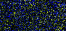
\includegraphics[width = .19\linewidth]{sb231_day_0}}
  \subcaptionbox{9 June\label{fig:day_24}}{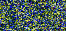
\includegraphics[width = .19\linewidth]{sb231_day_24}}
  \subcaptionbox{3 July\label{fig:day_48}}{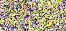
\includegraphics[width = .19\linewidth]{sb231_day_48}}
  \subcaptionbox{27 July\label{fig:day_72}}{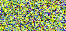
\includegraphics[width = .19\linewidth]{sb231_day_72}}
  \subcaptionbox{20 Aug.\label{fig:day_96}}{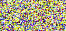
\includegraphics[width = .19\linewidth]{sb231_day_96}}
  \caption{Crop samples taken in 2016 over time, in Pauli decomposition}
  \label{fig:sample_images}
\end{figure}

We computed the distance of each pixel to all prototypes (except to $\bm K_{\text{dep}}$), and retained those closer to $\bm K_{\text{t}}$ than to the others.

\begin{figure*}[htb]
\centering
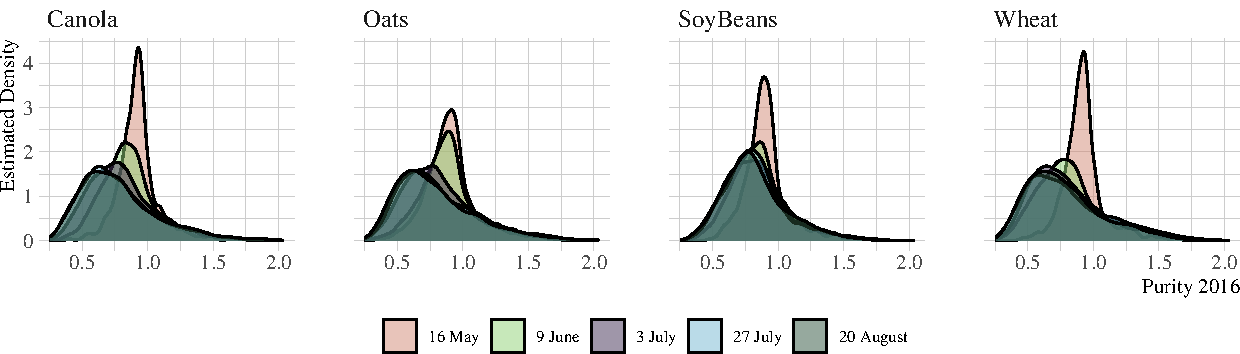
\includegraphics[width=\linewidth]{Purity}
\caption{Purity Indexes from Canola, Oats, Soy Beans, and Wheat in five dates}\label{fig:AllPurities}
\end{figure*}

\begin{figure}[hbt]
\centering
\subcaptionbox{Geodesic Purity Index $P_{\text{GD}}$}{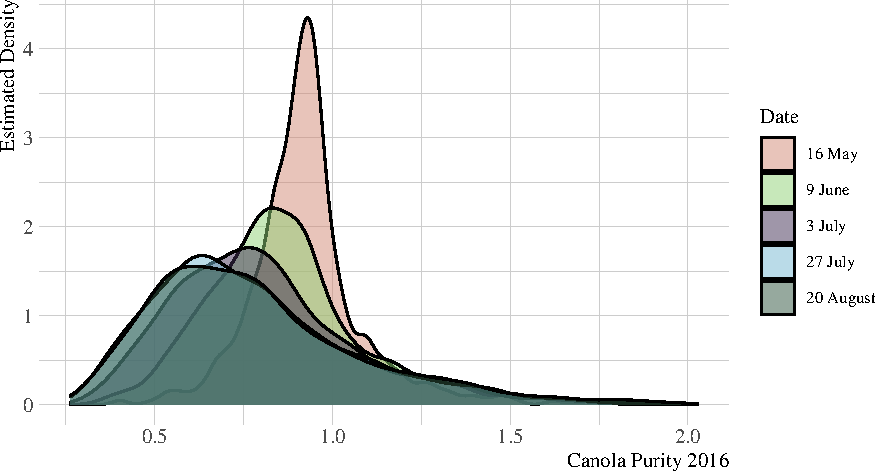
\includegraphics[width=\linewidth]{CanolaPurity}}
\subcaptionbox{Geodesic Type Scattering Angle $\alpha_{\text{GD}}$}{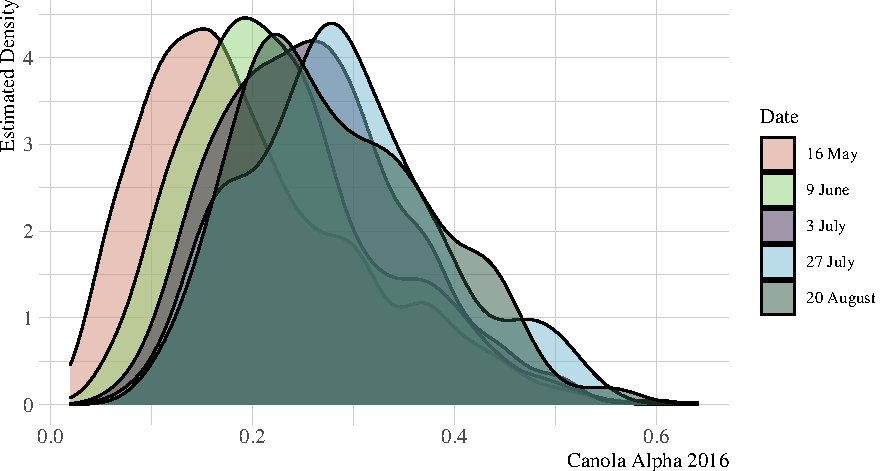
\includegraphics[width=\linewidth]{CanolaAlpha}}
\subcaptionbox{Geodesic Helicity $\tau_{\text{GD}}$}{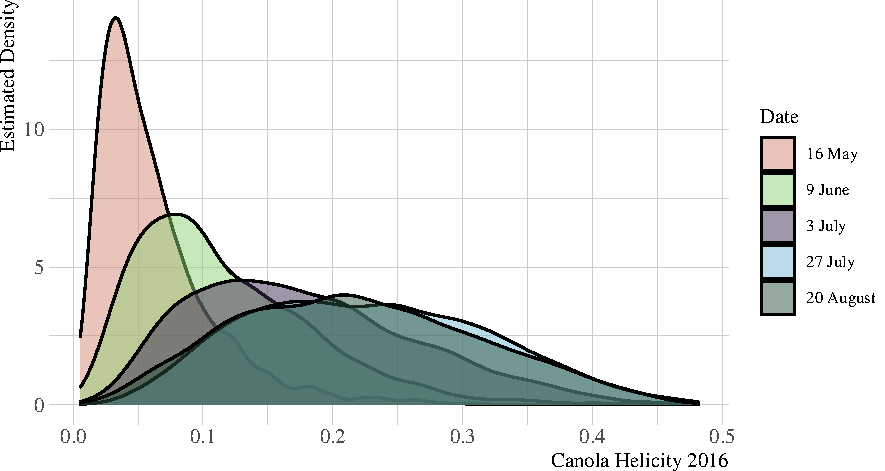
\includegraphics[width=\linewidth]{CanolaHelicity}}
\caption{Geodesic Indexes for Canola\label{fig:CanolaIndexes}}
\end{figure}

\textcolor{red}{\hrulefill}

From this selected distances per image, it was generated the histograms shown in the figure \ref{fig:histograms_alpha_sb231}. Through these graphs, one can suppose that these data obey a Beta distribution. To evaluate this assumption, the Komolgorov-Smirnov test was performed, whose $p$-values are in the table \ref{tab:pvalues_alpha_sb231} along with the sample size.

The roadmap for the data analysis of these images is:
\begin{enumerate}
  \item Obtaining the geodesic purity index and scattering type angle of the data;
  \item Making a descriptive analysis of the data with histograms and boxplots;
  \item Fitting the data with models;
  \item Making separability tests.
\end{enumerate}


% A first inspection of the purity indexes suggested that Beta distributions may be a good explanatory model.
% The data look crammed in their original space, though.
% 
% After this initial qualitative analysis, we decided to transform the data applying the logarithmic function.
% Fig.~\ref{fig:histograms_purity_sb231} shows the histograms and boxplots. 
% The closeness to Gaussian distributions is remarkable.
% The QQ-Plots shown in Fig.~\ref{fig:qqplots} provide more evidence of such good adherence.
% Table~\ref{tab:pvalues_purities_sb231} provides the $p$-values of the Shapiro-Wilk test of goodness-of-fit to the Gaussian distribution.
% There is no evidence, thus, to reject the hypothesis that the log-transformed purity data follows Gaussian distributions.

% \begin{figure}[hbt]
%     \centering
%     \subcaptionbox{16 May 2016}{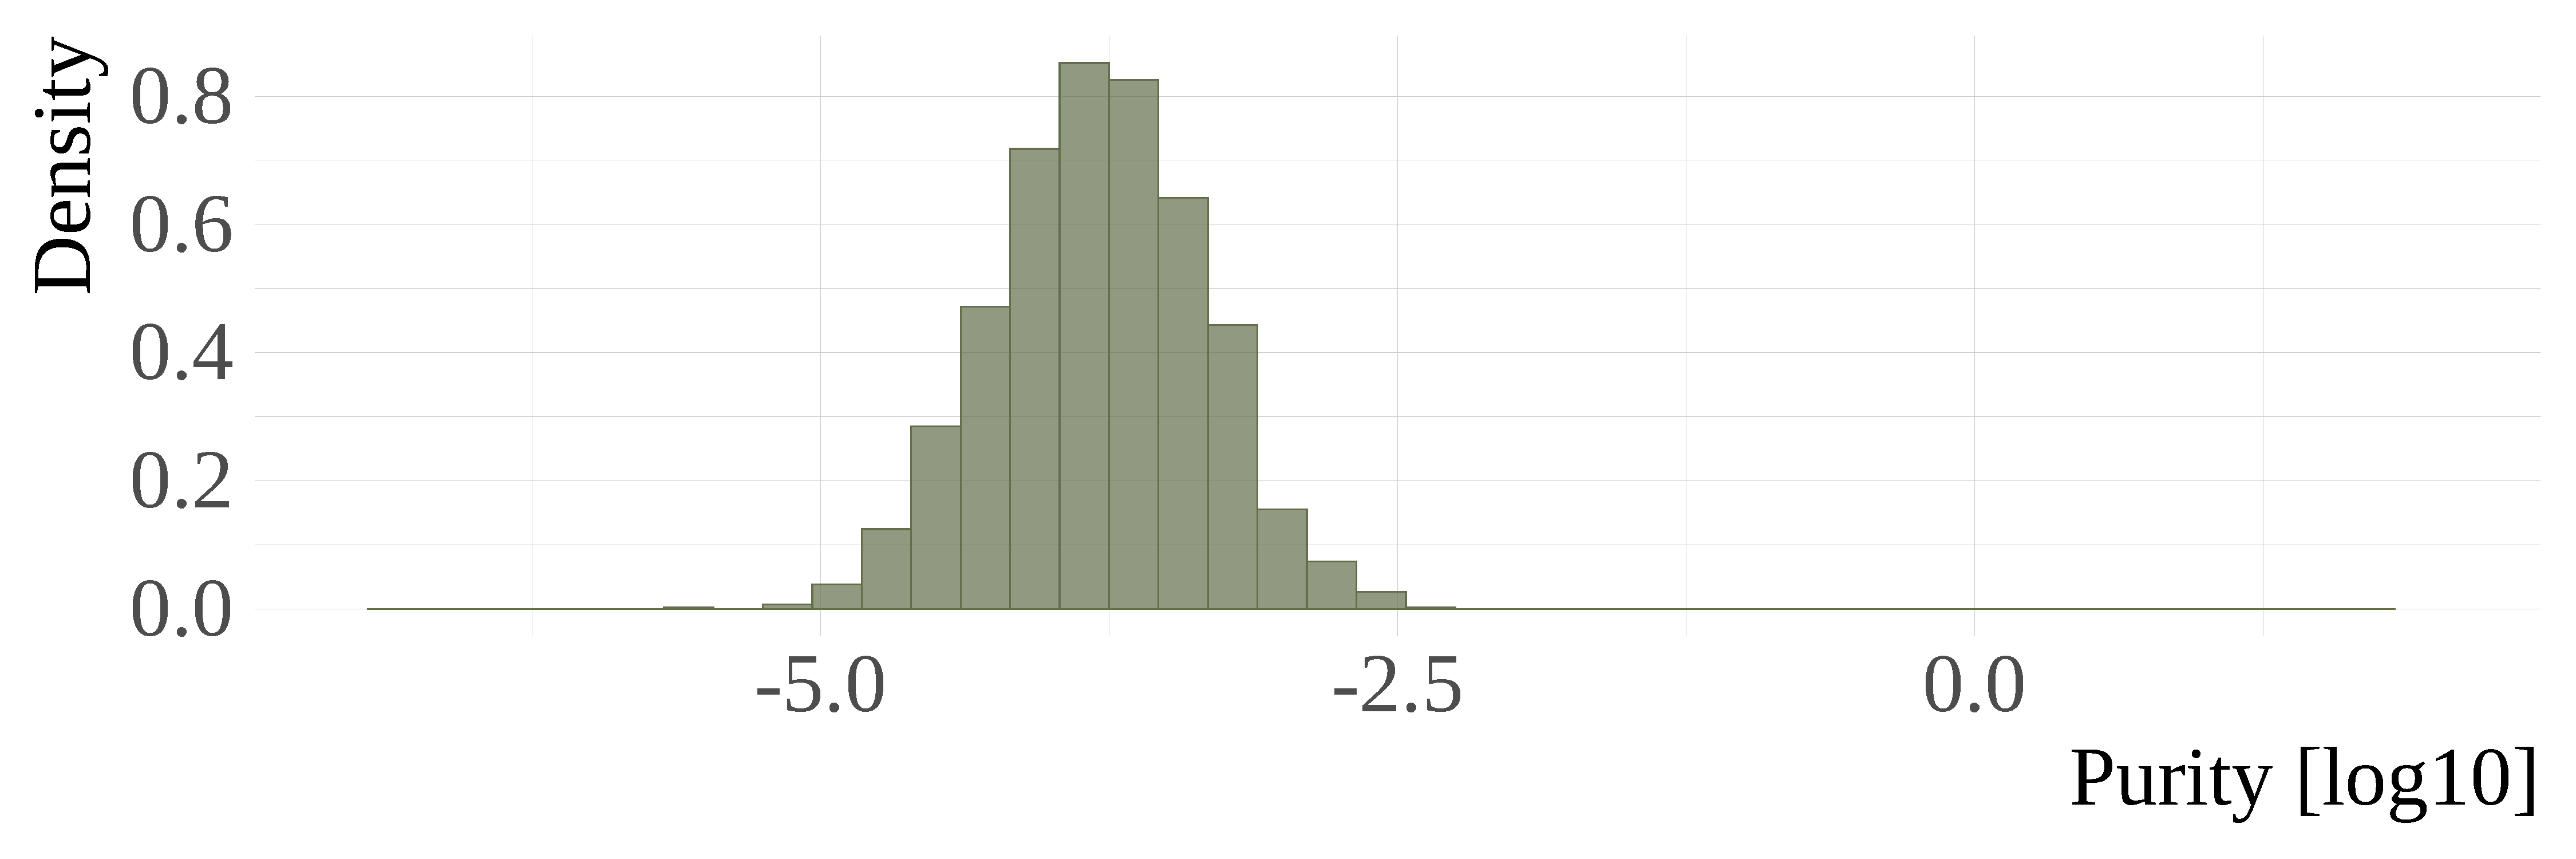
\includegraphics[width = \linewidth]{Figures/Soybeans_231/log_purity_sb231_1}}
%     \subcaptionbox{09 June 2016}{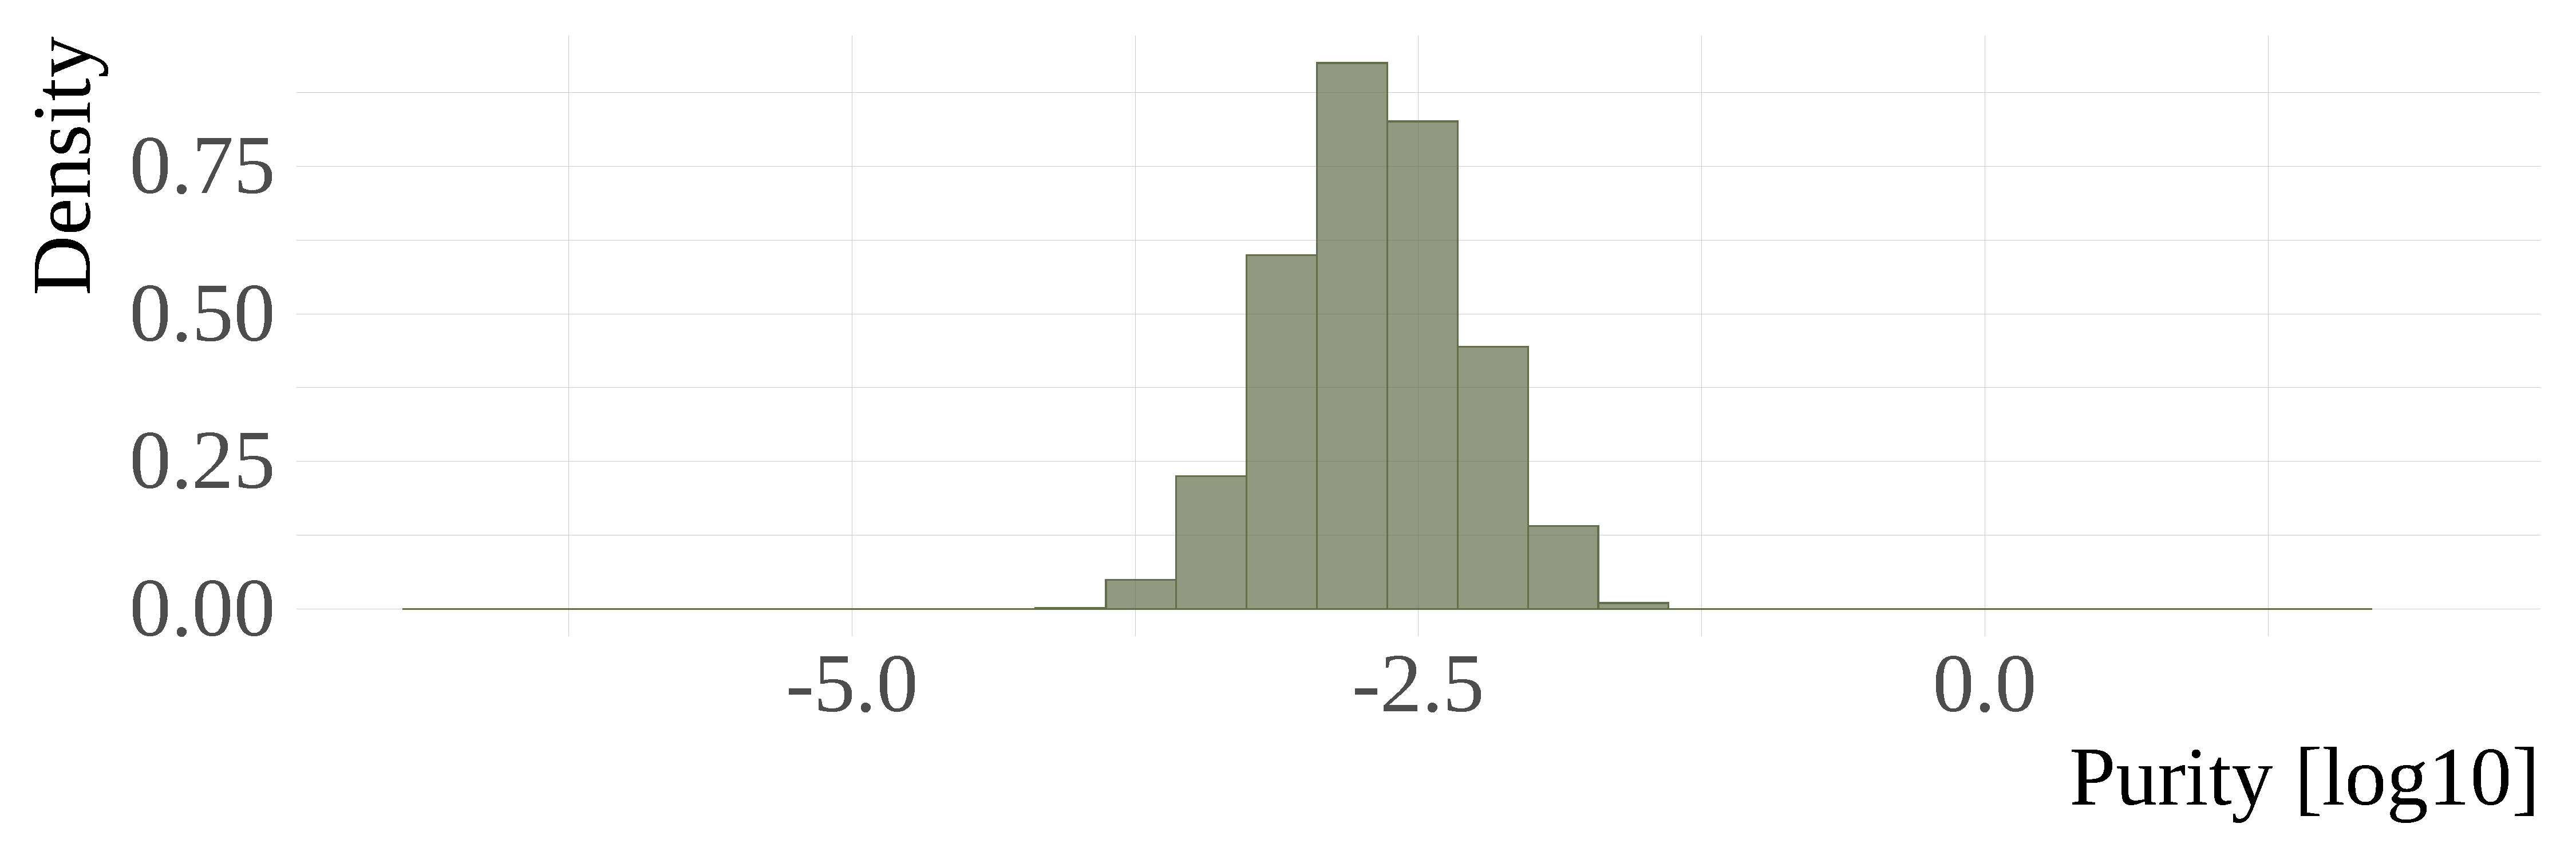
\includegraphics[width = \linewidth]{Figures/Soybeans_231/log_purity_sb231_2}}
%     \subcaptionbox{03 July 2016}{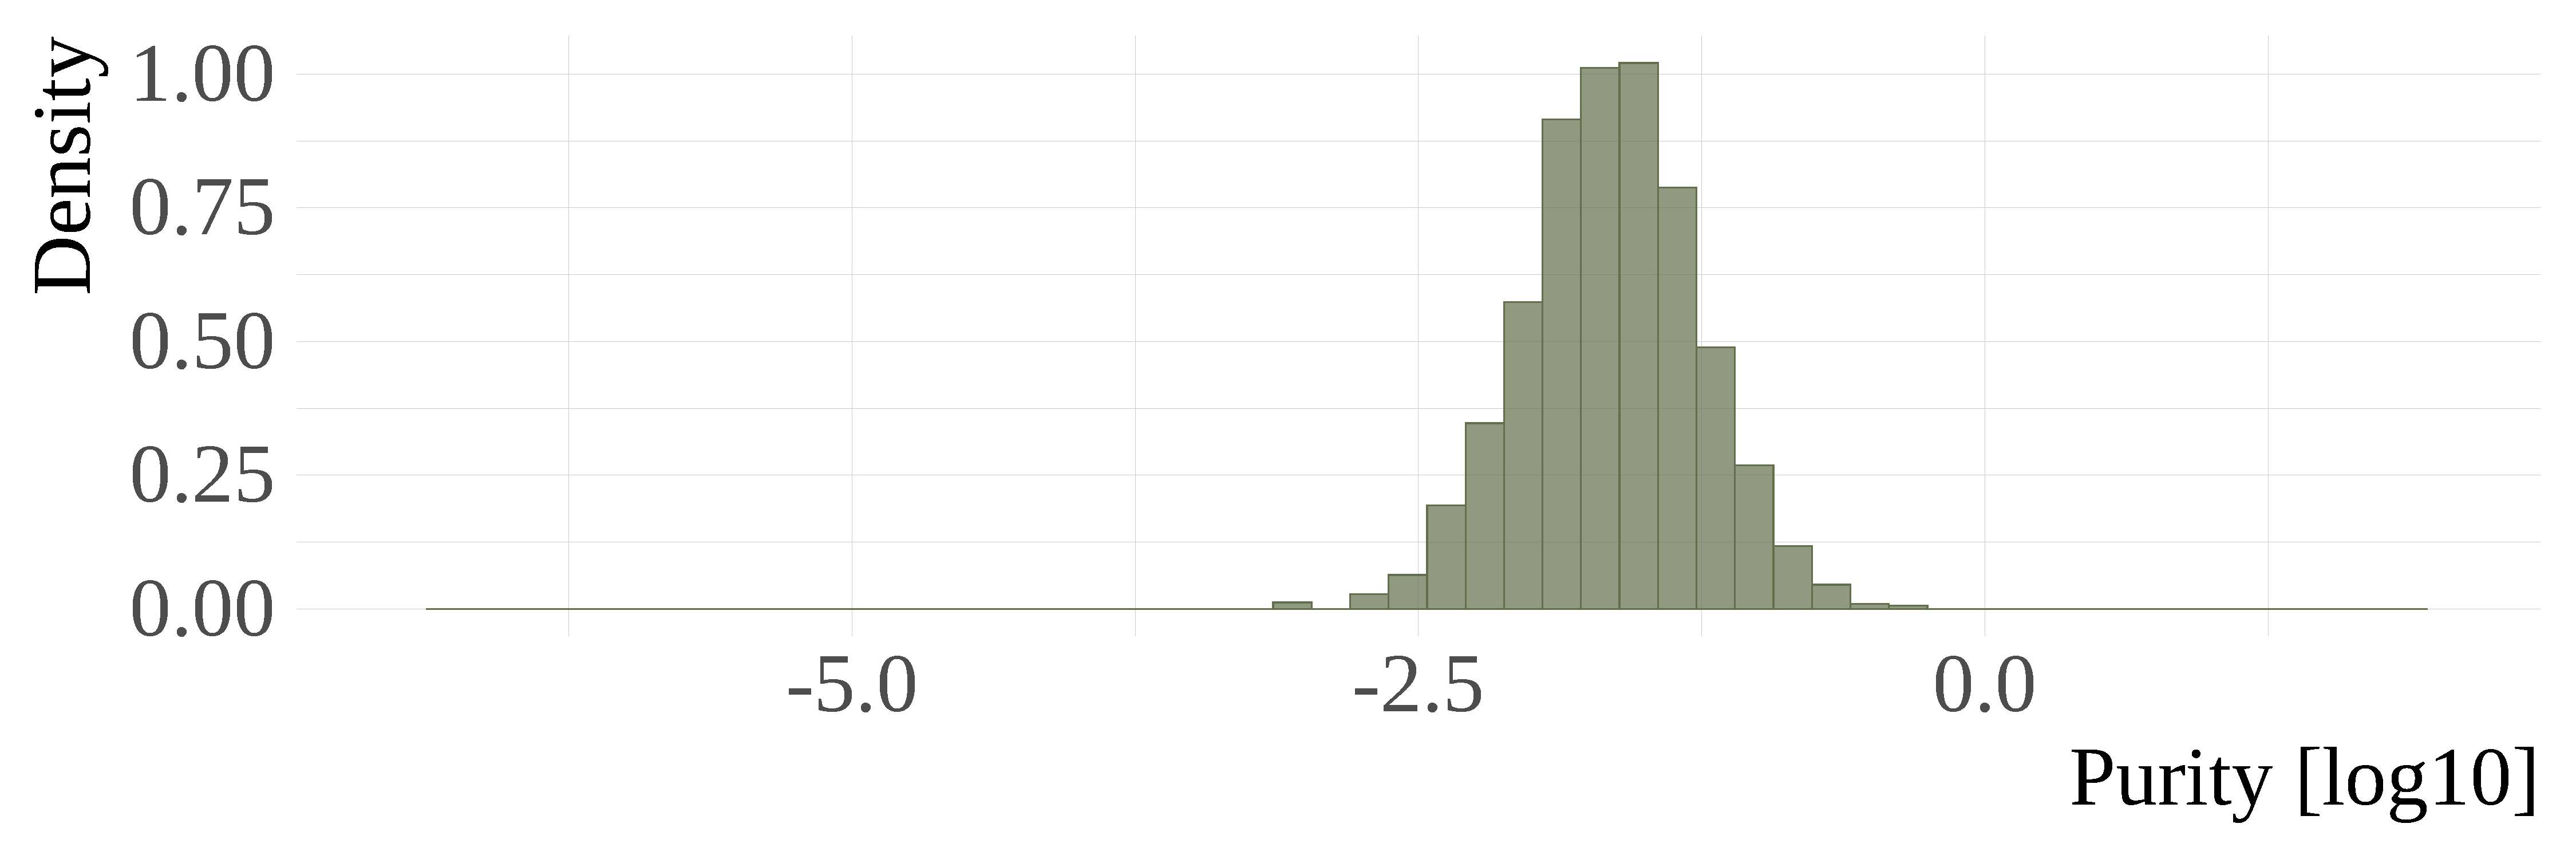
\includegraphics[width = \linewidth]{Figures/Soybeans_231/log_purity_sb231_3}}
%     \subcaptionbox{27 July 2016}{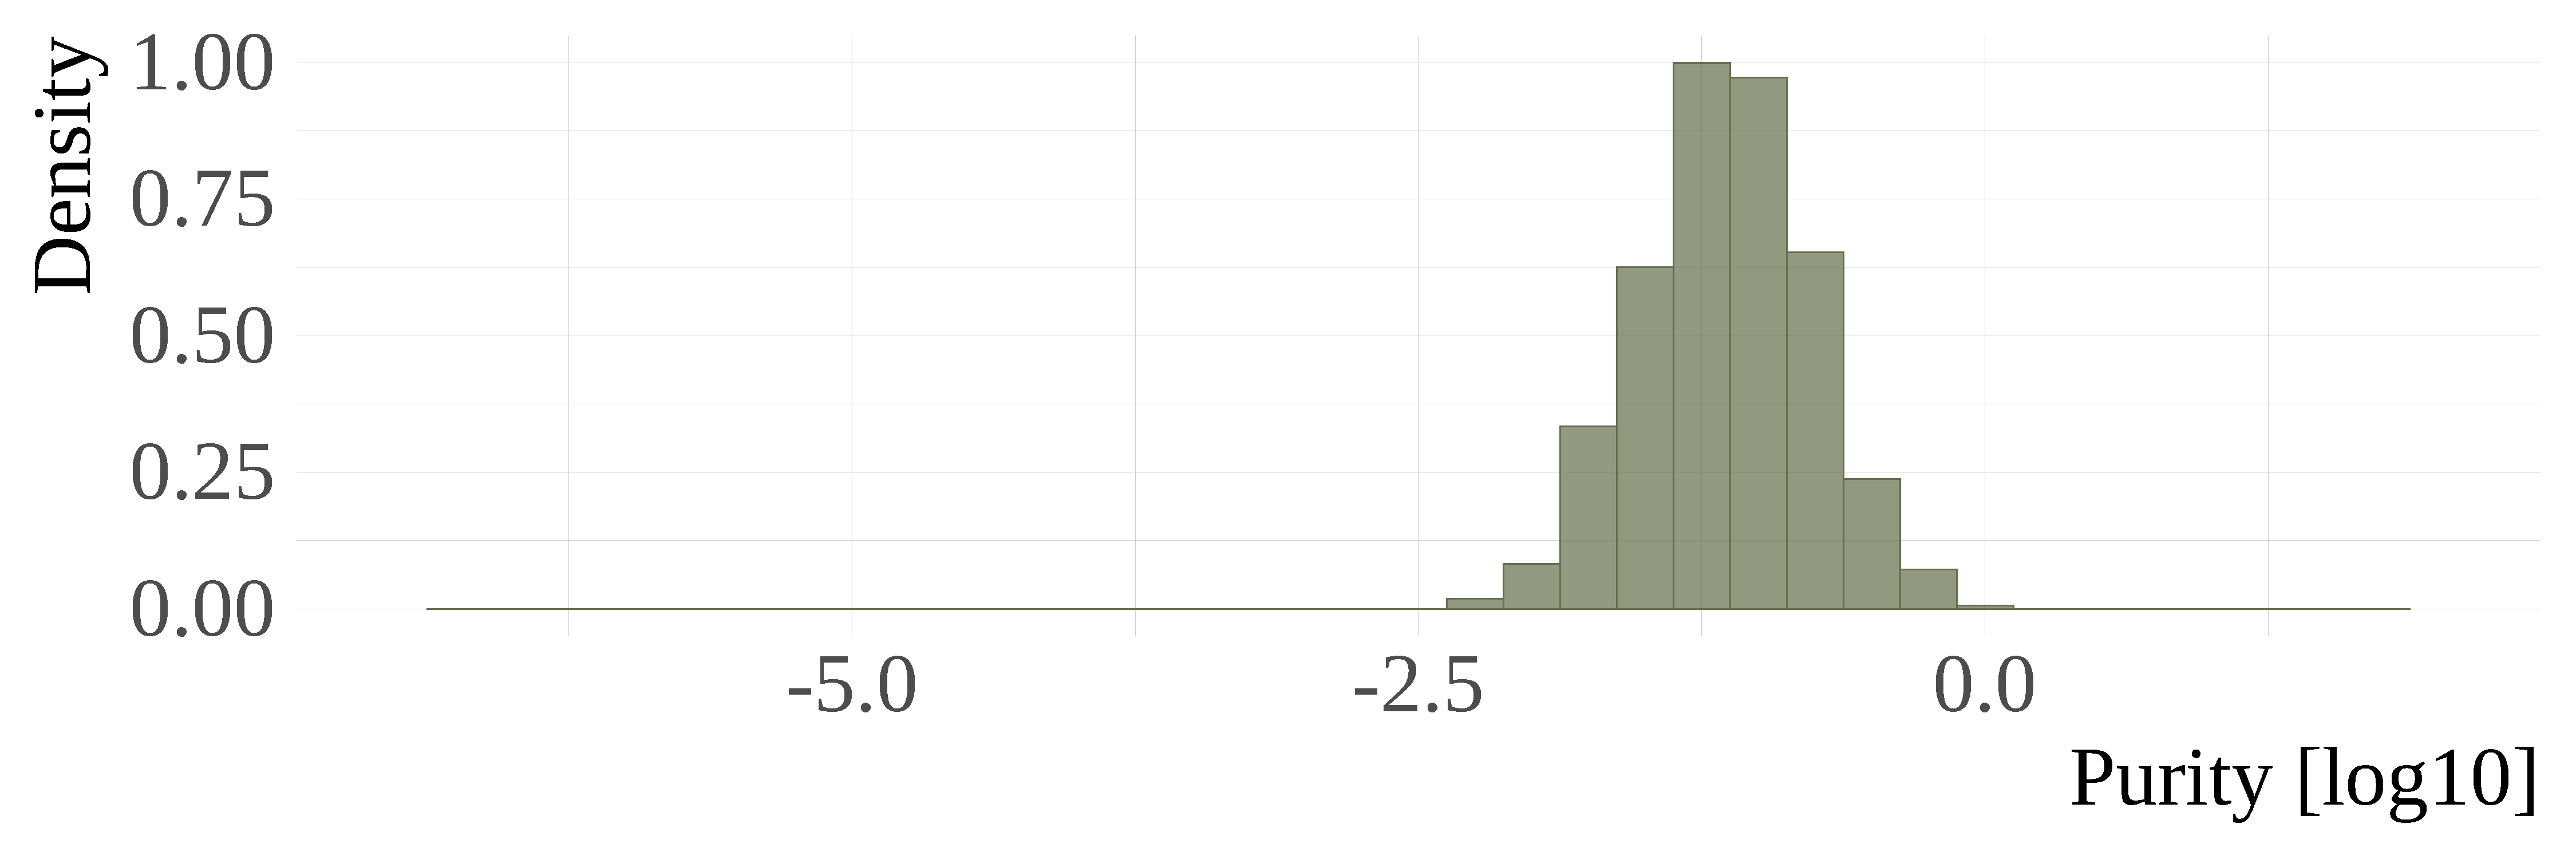
\includegraphics[width = \linewidth]{Figures/Soybeans_231/log_purity_sb231_4}}
%     \subcaptionbox{20 August 2016}{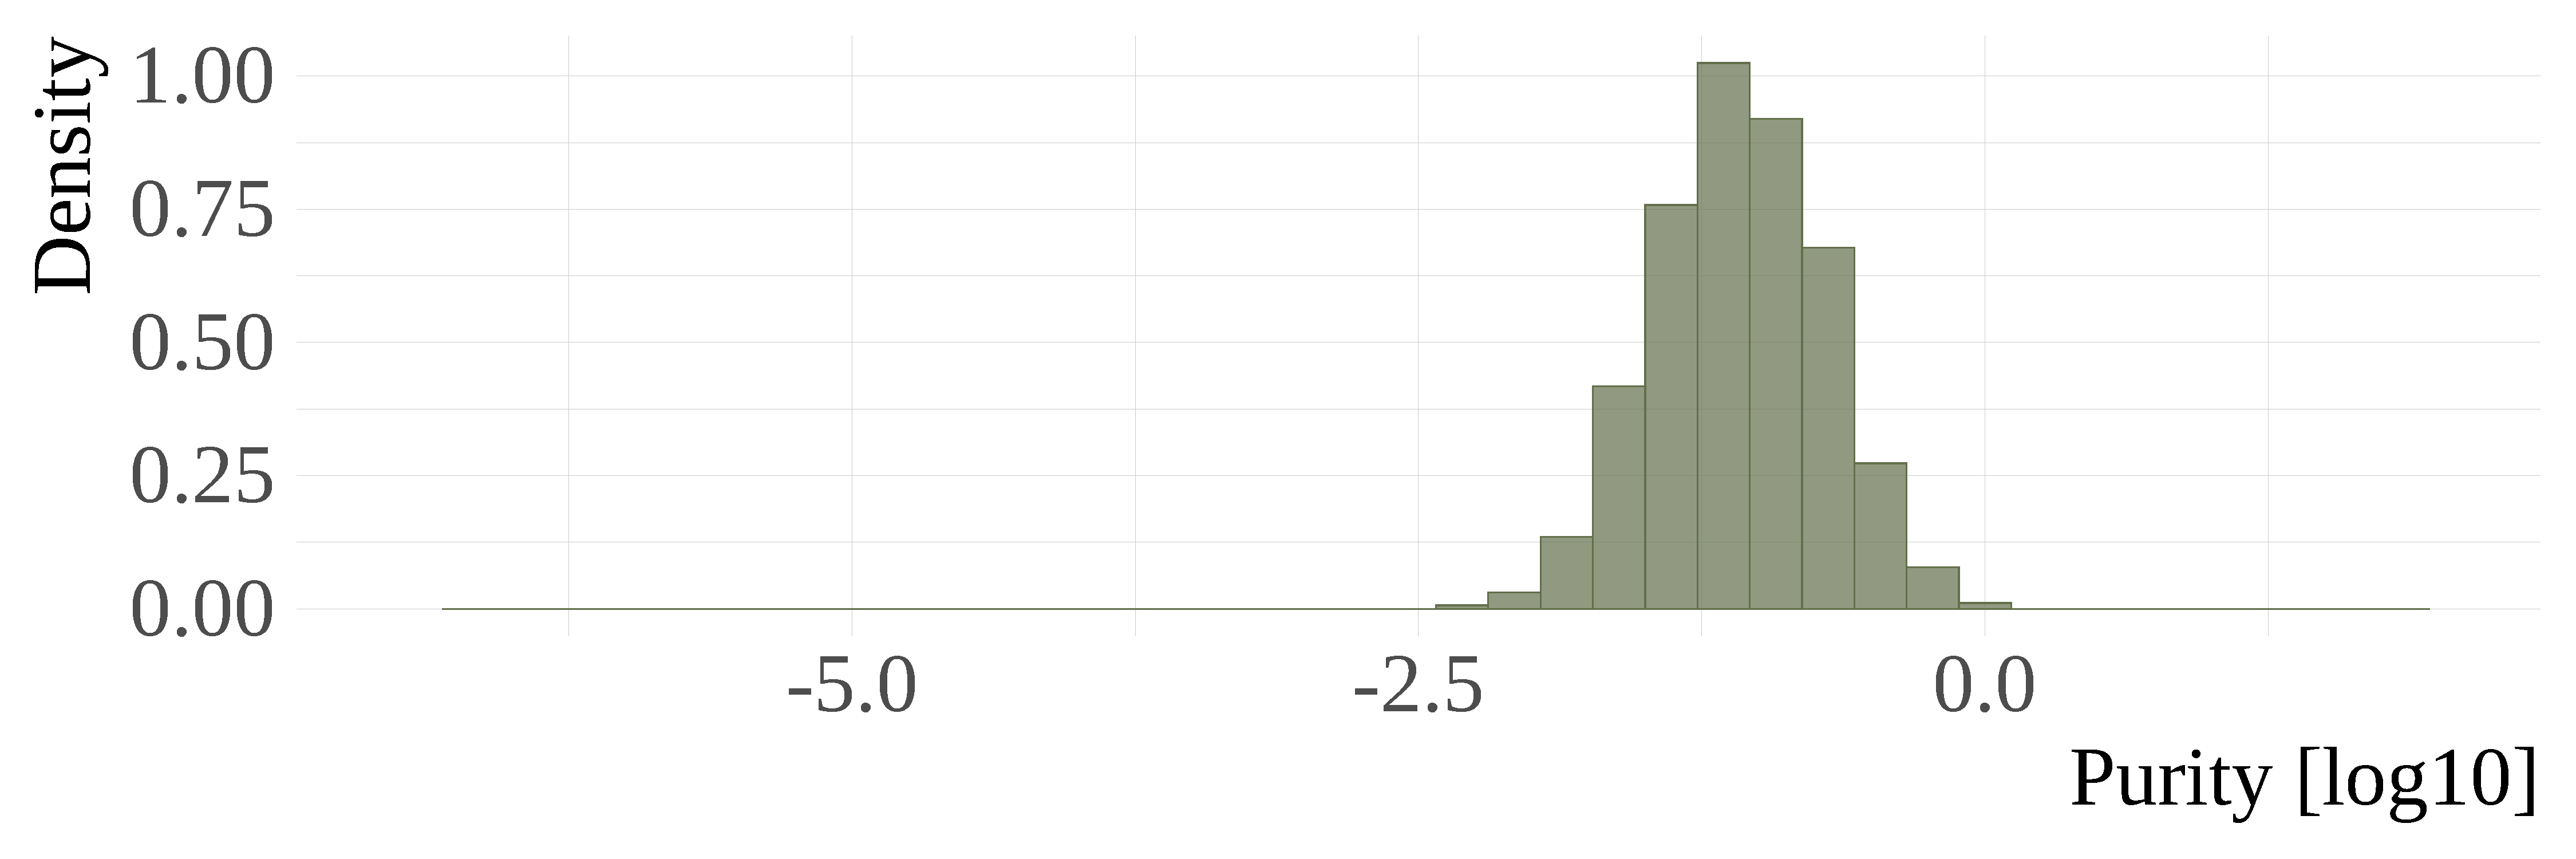
\includegraphics[width = \linewidth]{Figures/Soybeans_231/log_purity_sb231_5}}
%     \caption{Histograms of the $log10$ of geodesic purity index from Soybeans 231}
%     \label{fig:histograms_purity_sb231}
% \end{figure}

% \begin{figure}[hbt]
%     \centering
%     \subcaptionbox{16 May 2016}{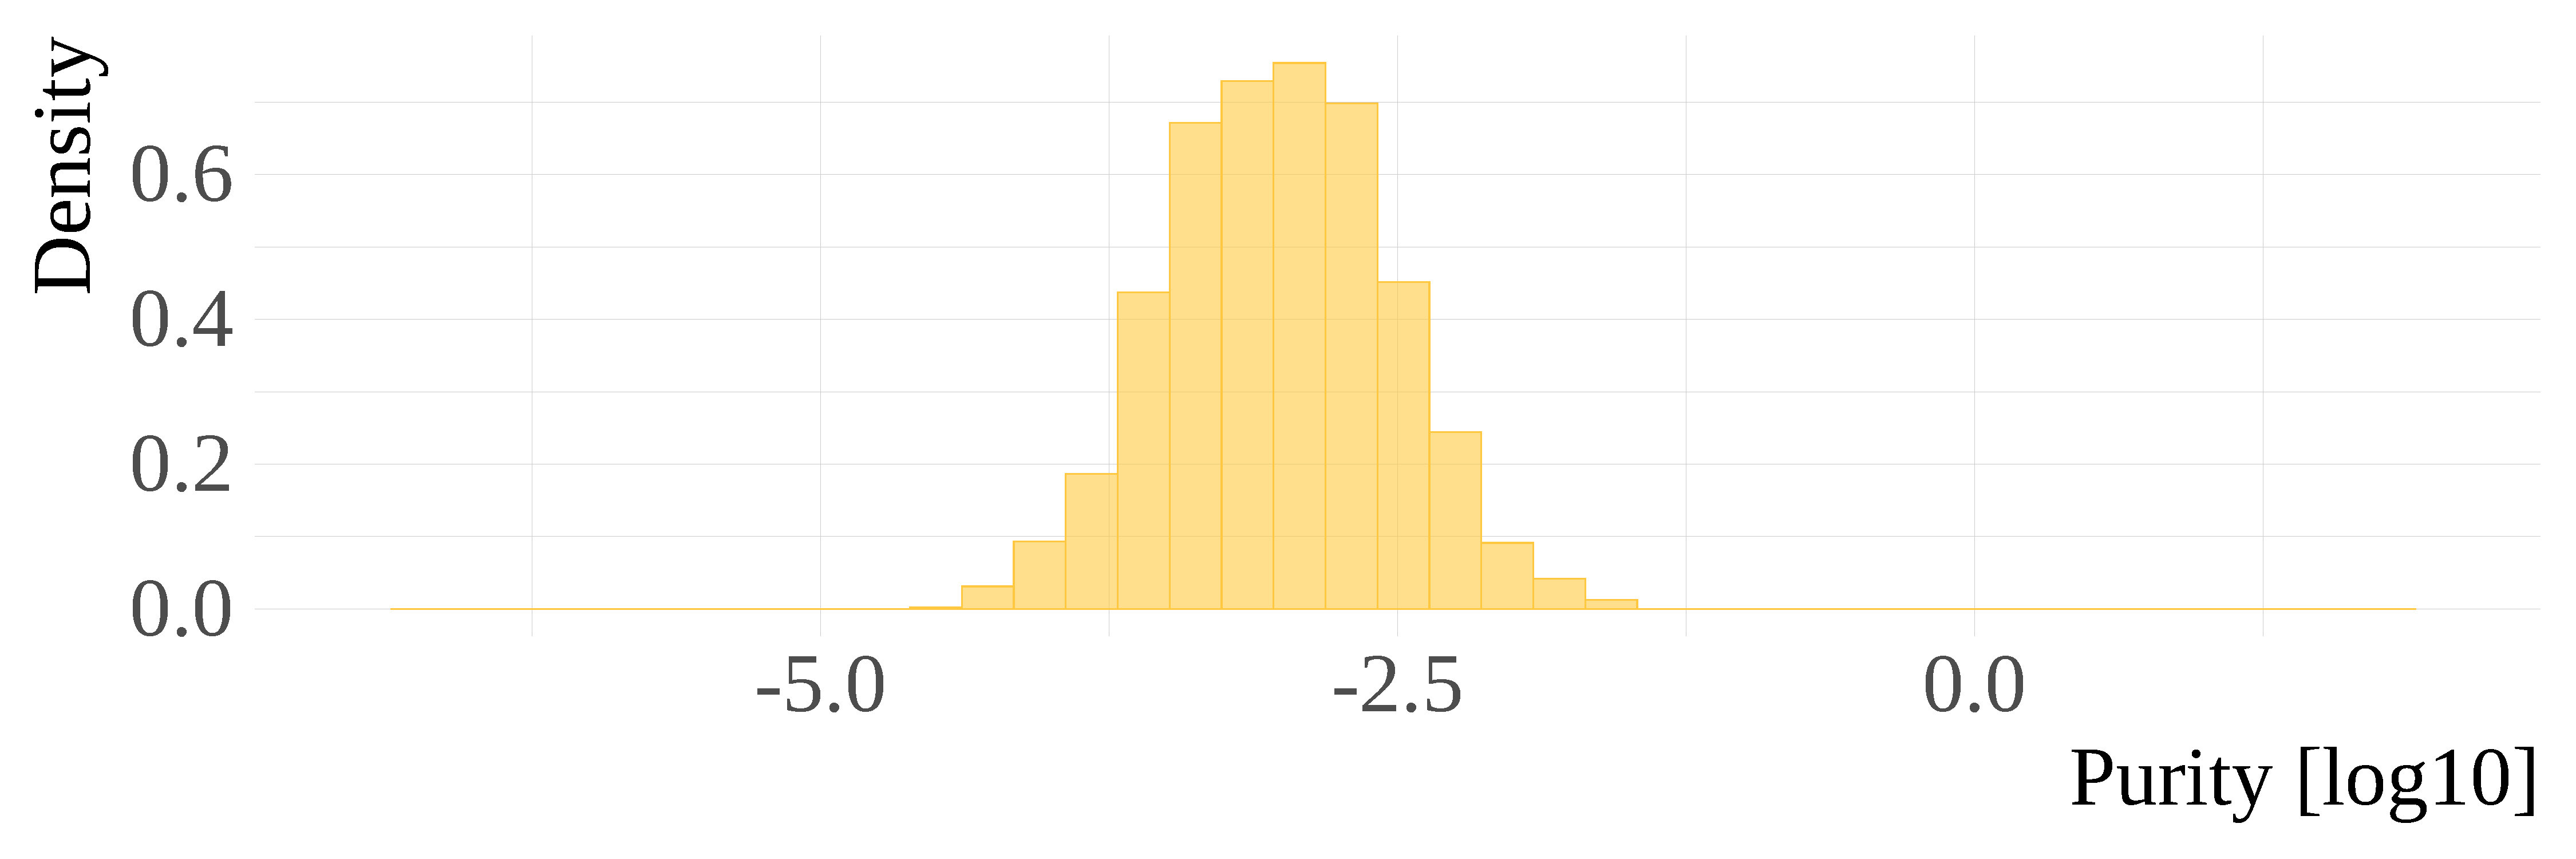
\includegraphics[width = \linewidth]{Figures/Canola_43/log_purity_cn43_1}}
%     \subcaptionbox{09 June 2016}{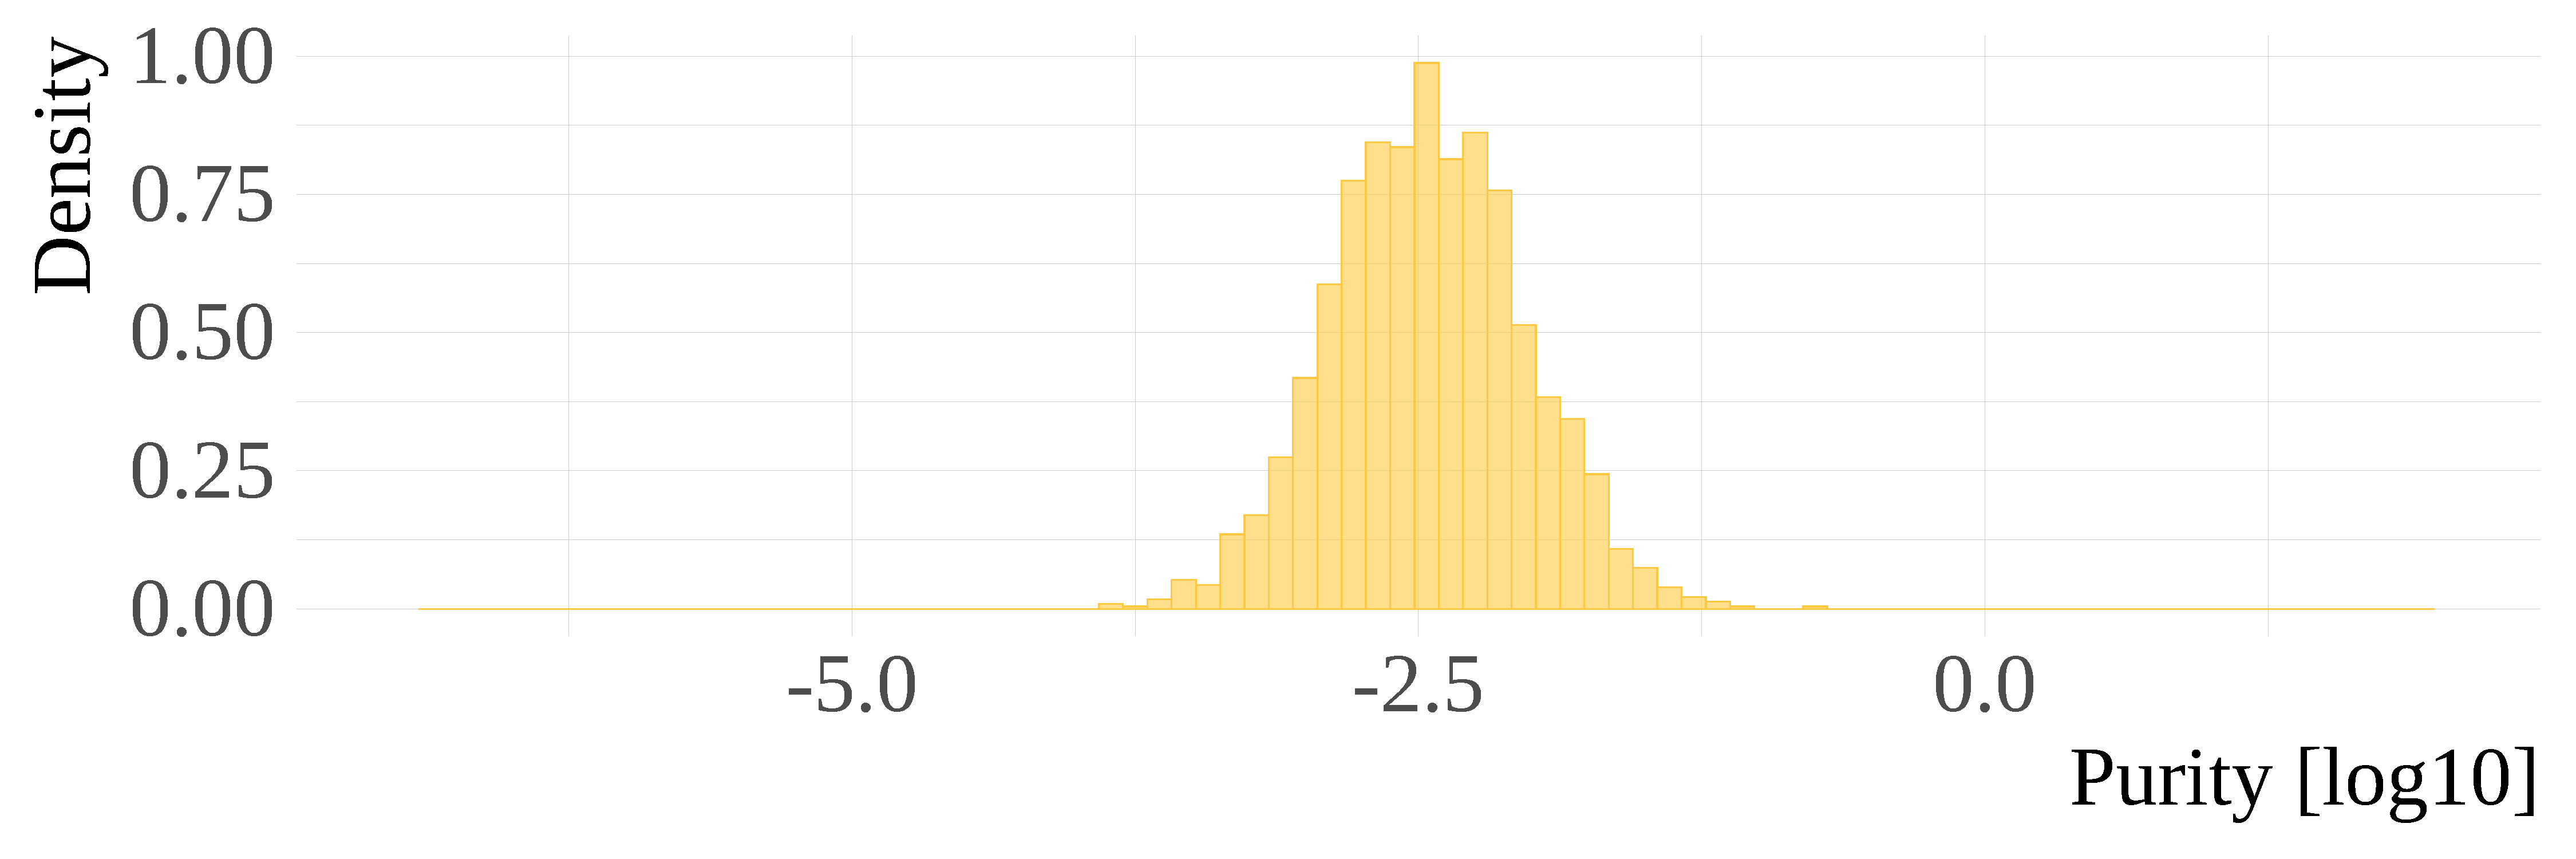
\includegraphics[width = \linewidth]{Figures/Canola_43/log_purity_cn43_2}}
%     \subcaptionbox{03 July 2016}{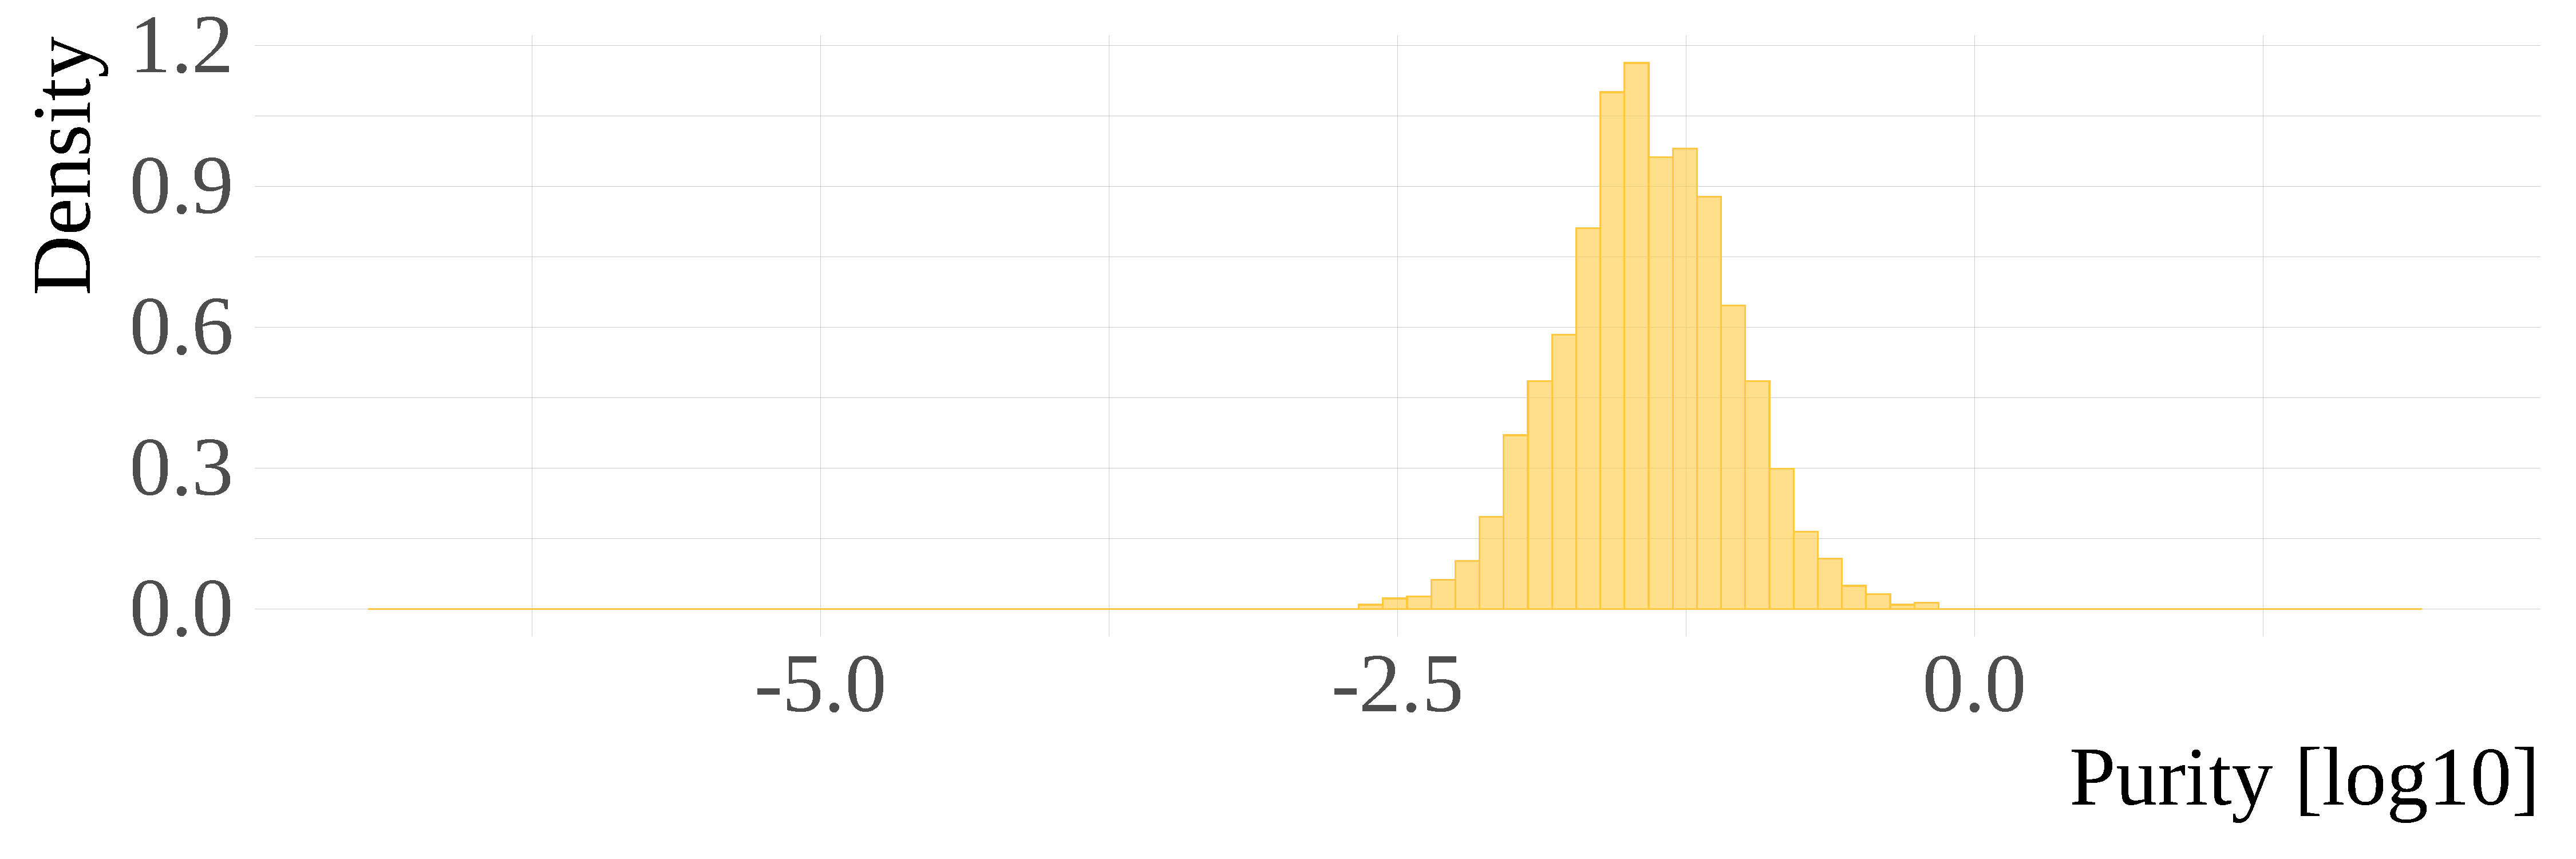
\includegraphics[width = \linewidth]{Figures/Canola_43/log_purity_cn43_3}}
%     \subcaptionbox{27 July 2016}{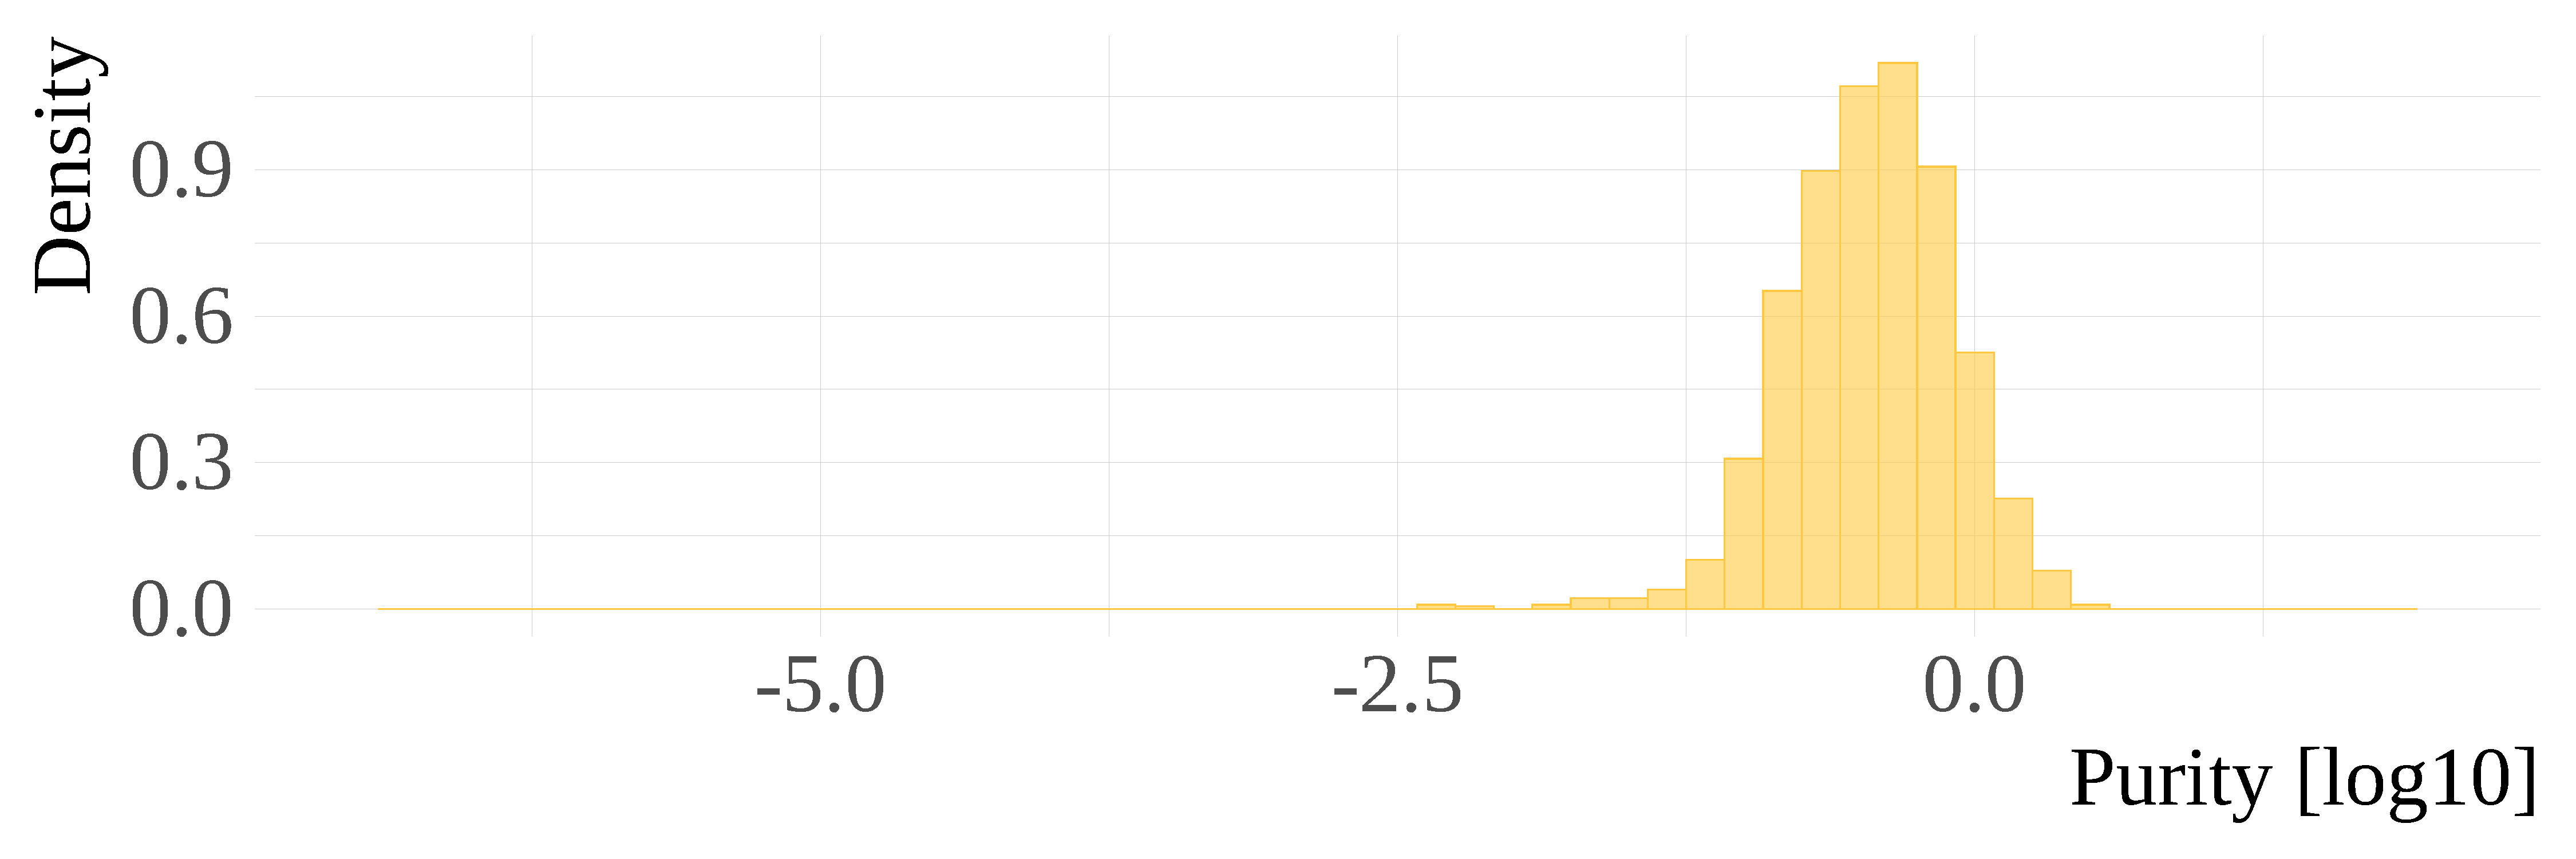
\includegraphics[width = \linewidth]{Figures/Canola_43/log_purity_cn43_4}}
%     \subcaptionbox{20 August 2016}{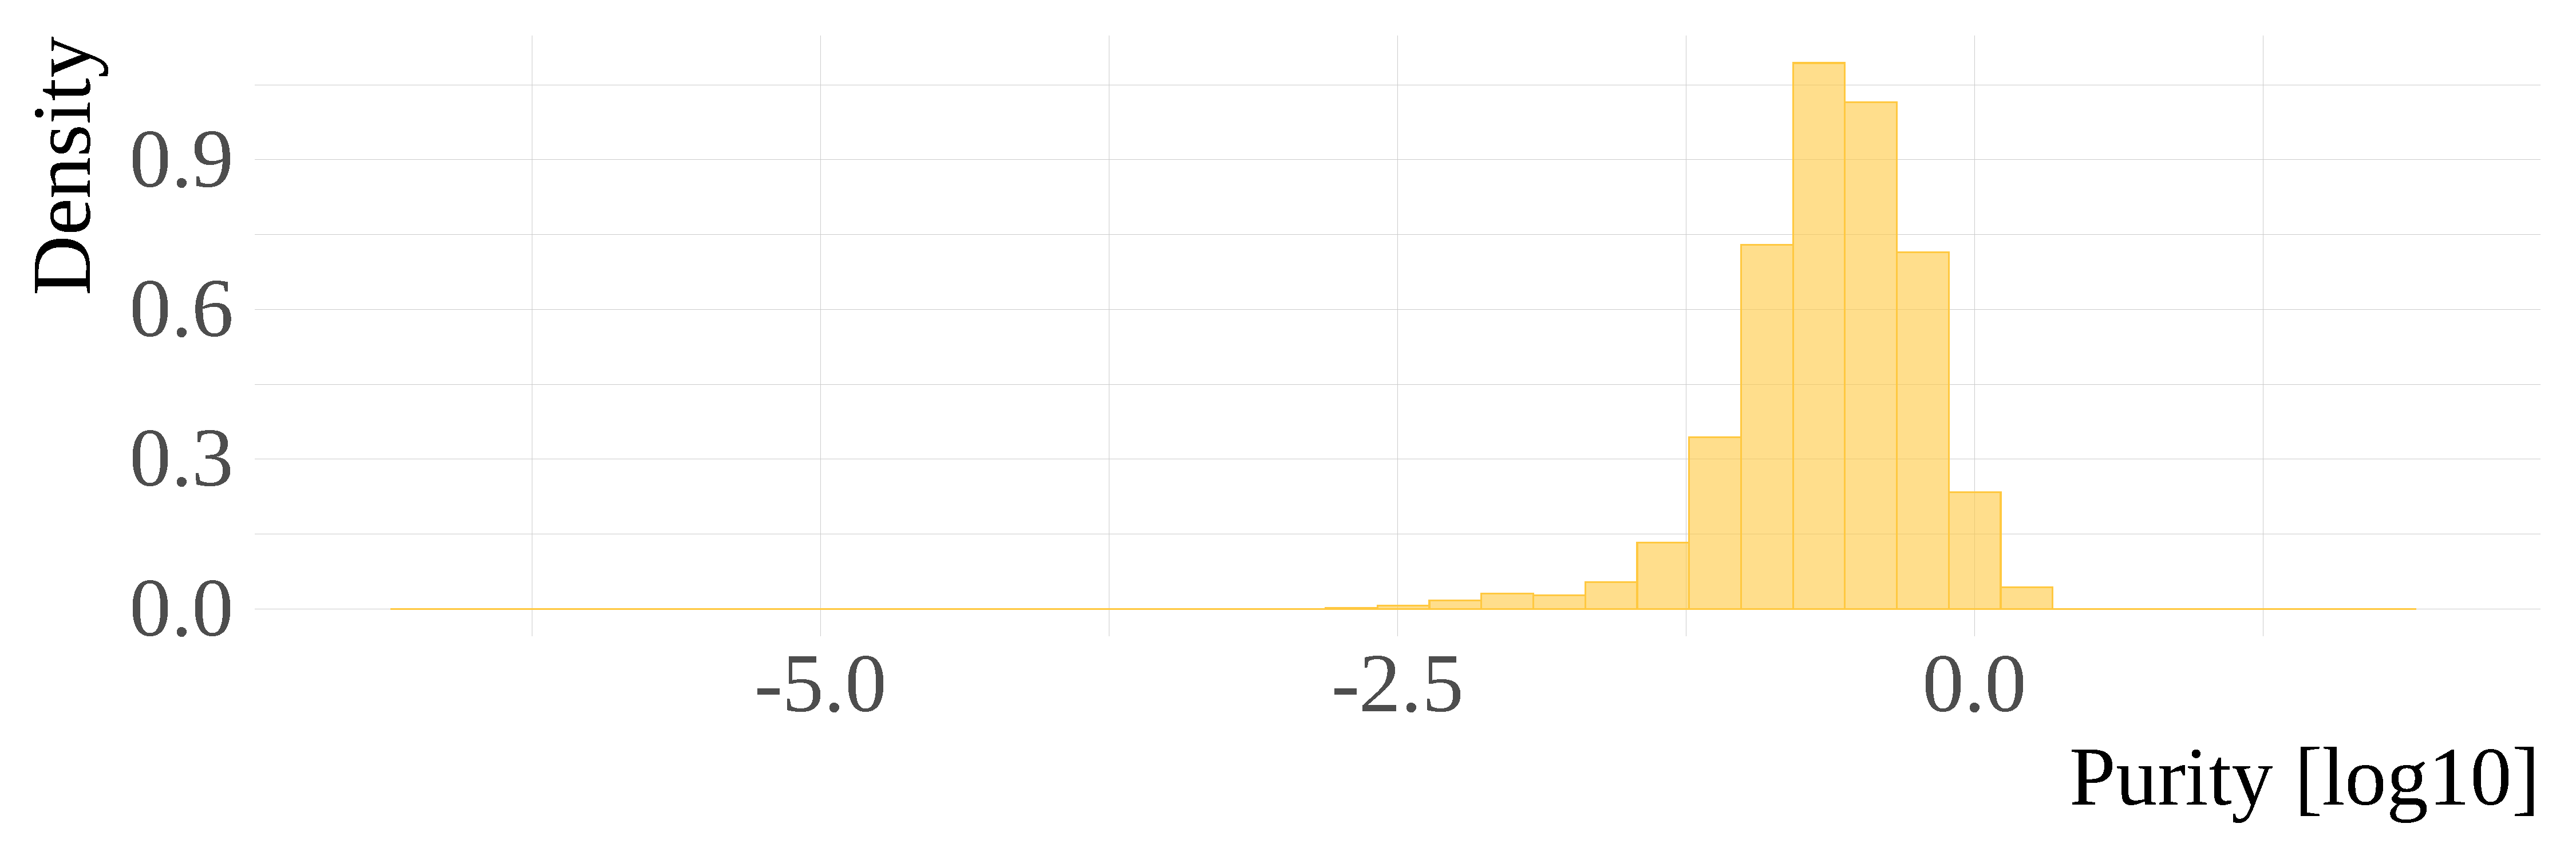
\includegraphics[width = \linewidth]{Figures/Canola_43/log_purity_cn43_5}}
%     \caption{Histograms of the $log10$ of geodesic purity index from Canola 43}
%     \label{fig:histograms_purity_cn43}
% \end{figure}

% \begin{figure}[hbt]
%     \centering
%     \subcaptionbox{16 May 2016}{\includegraphics[width = \linewidth]{Figures/Wheat_104/log_purity_wt104_1}}
%     \subcaptionbox{09 June 2016}{\includegraphics[width = \linewidth]{Figures/Wheat_104/log_purity_wt104_2}}
%     \subcaptionbox{03 July 2016}{\includegraphics[width = \linewidth]{Figures/Wheat_104/log_purity_wt104_3}}
%     \subcaptionbox{27 July 2016}{\includegraphics[width = \linewidth]{Figures/Wheat_104/log_purity_wt104_4}}
%     \subcaptionbox{20 August 2016}{\includegraphics[width = \linewidth]{Figures/Wheat_104/log_purity_wt104_5}}
%     \caption{Histograms of the $log10$ of geodesic purity index from Wheat 104}
%     \label{fig:histograms_purity_wt104}
% \end{figure}

% \begin{figure}[hbt]
%     \centering
%     \subcaptionbox{16 May 2016}{\includegraphics[width = \linewidth]{Figures/Oats_102/log_purity_ot102_1}}
%     \subcaptionbox{09 June 2016}{\includegraphics[width = \linewidth]{Figures/Oats_102/log_purity_ot102_2}}
%     \subcaptionbox{03 July 2016}{\includegraphics[width = \linewidth]{Figures/Oats_102/log_purity_ot102_3}}
%     \subcaptionbox{27 July 2016}{\includegraphics[width = \linewidth]{Figures/Oats_102/log_purity_ot102_4}}
%     \subcaptionbox{20 August 2016}{\includegraphics[width = \linewidth]{Figures/Oats_102/log_purity_ot102_5}}
%     \caption{Histograms of the $log10$ of geodesic purity index from Oats 102}
%     \label{fig:histograms_purity_ot102}
% \end{figure}

%\begin{figure}[hbt]
%  \centering
%  \subcaptionbox{Histograms\label{fig:histograms_purity}}{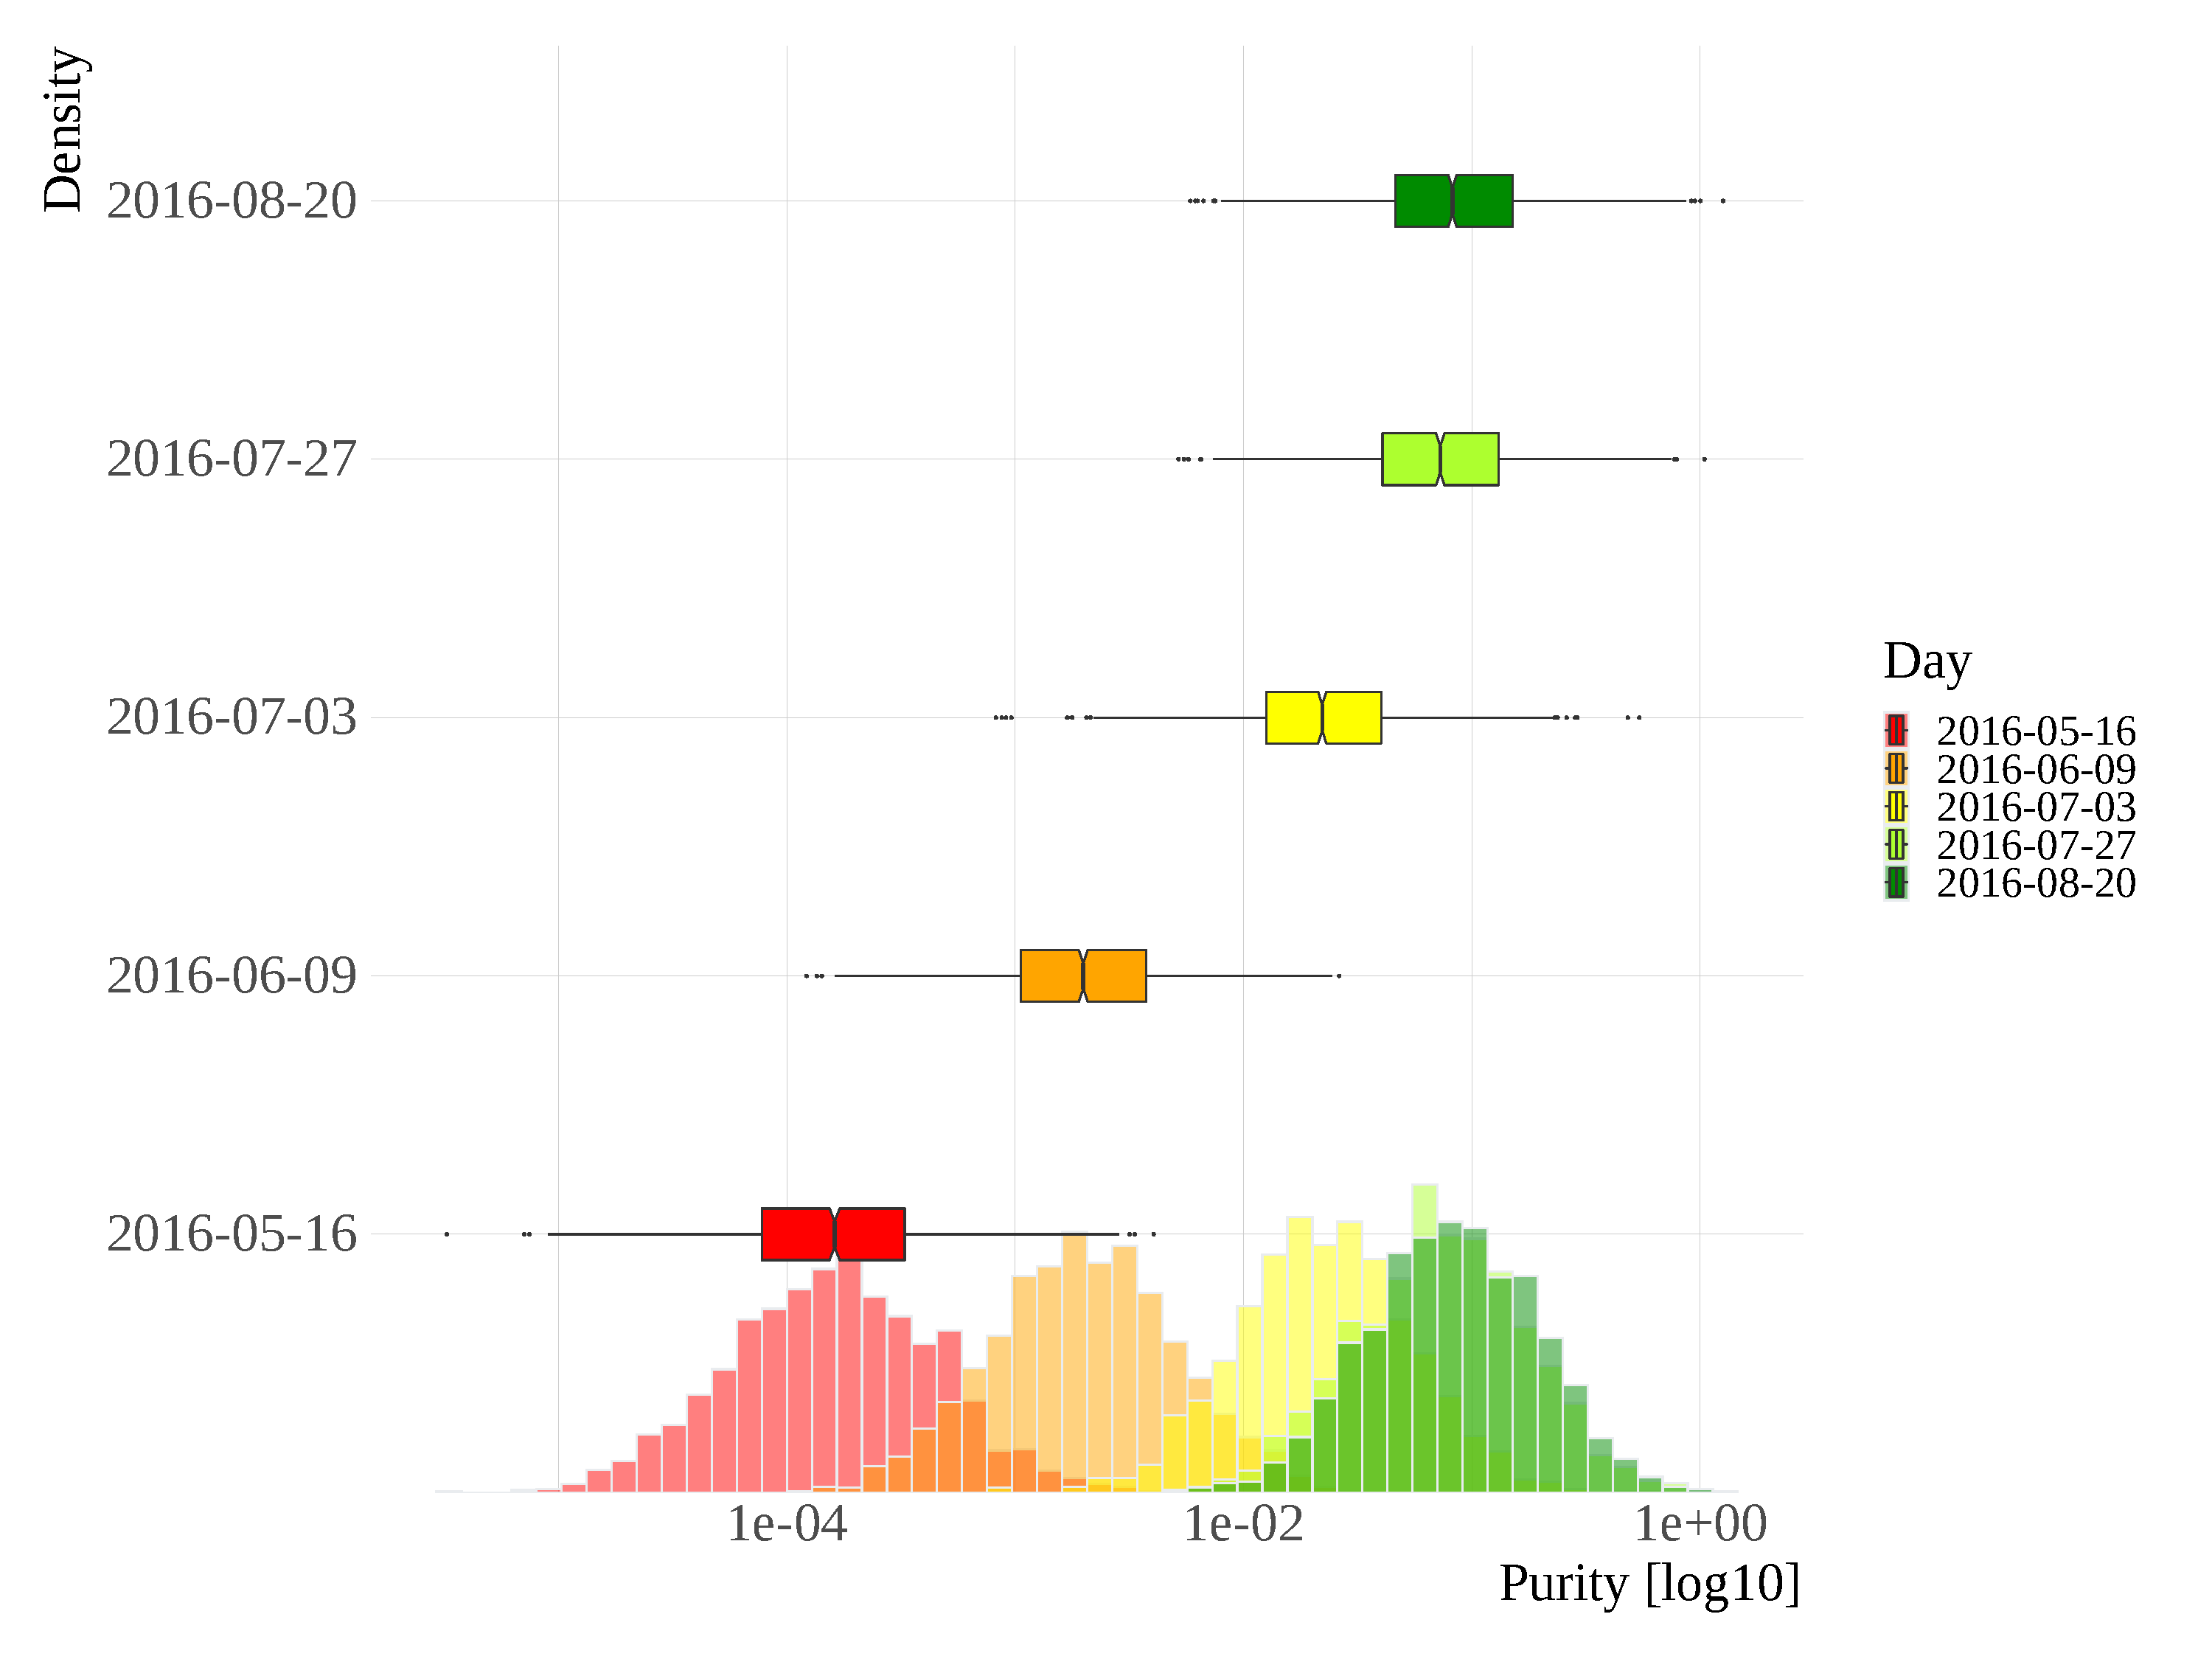
\includegraphics[width = .95\linewidth]{histograms}}
%  \subcaptionbox{QQPlots\label{fig:qqplots}}{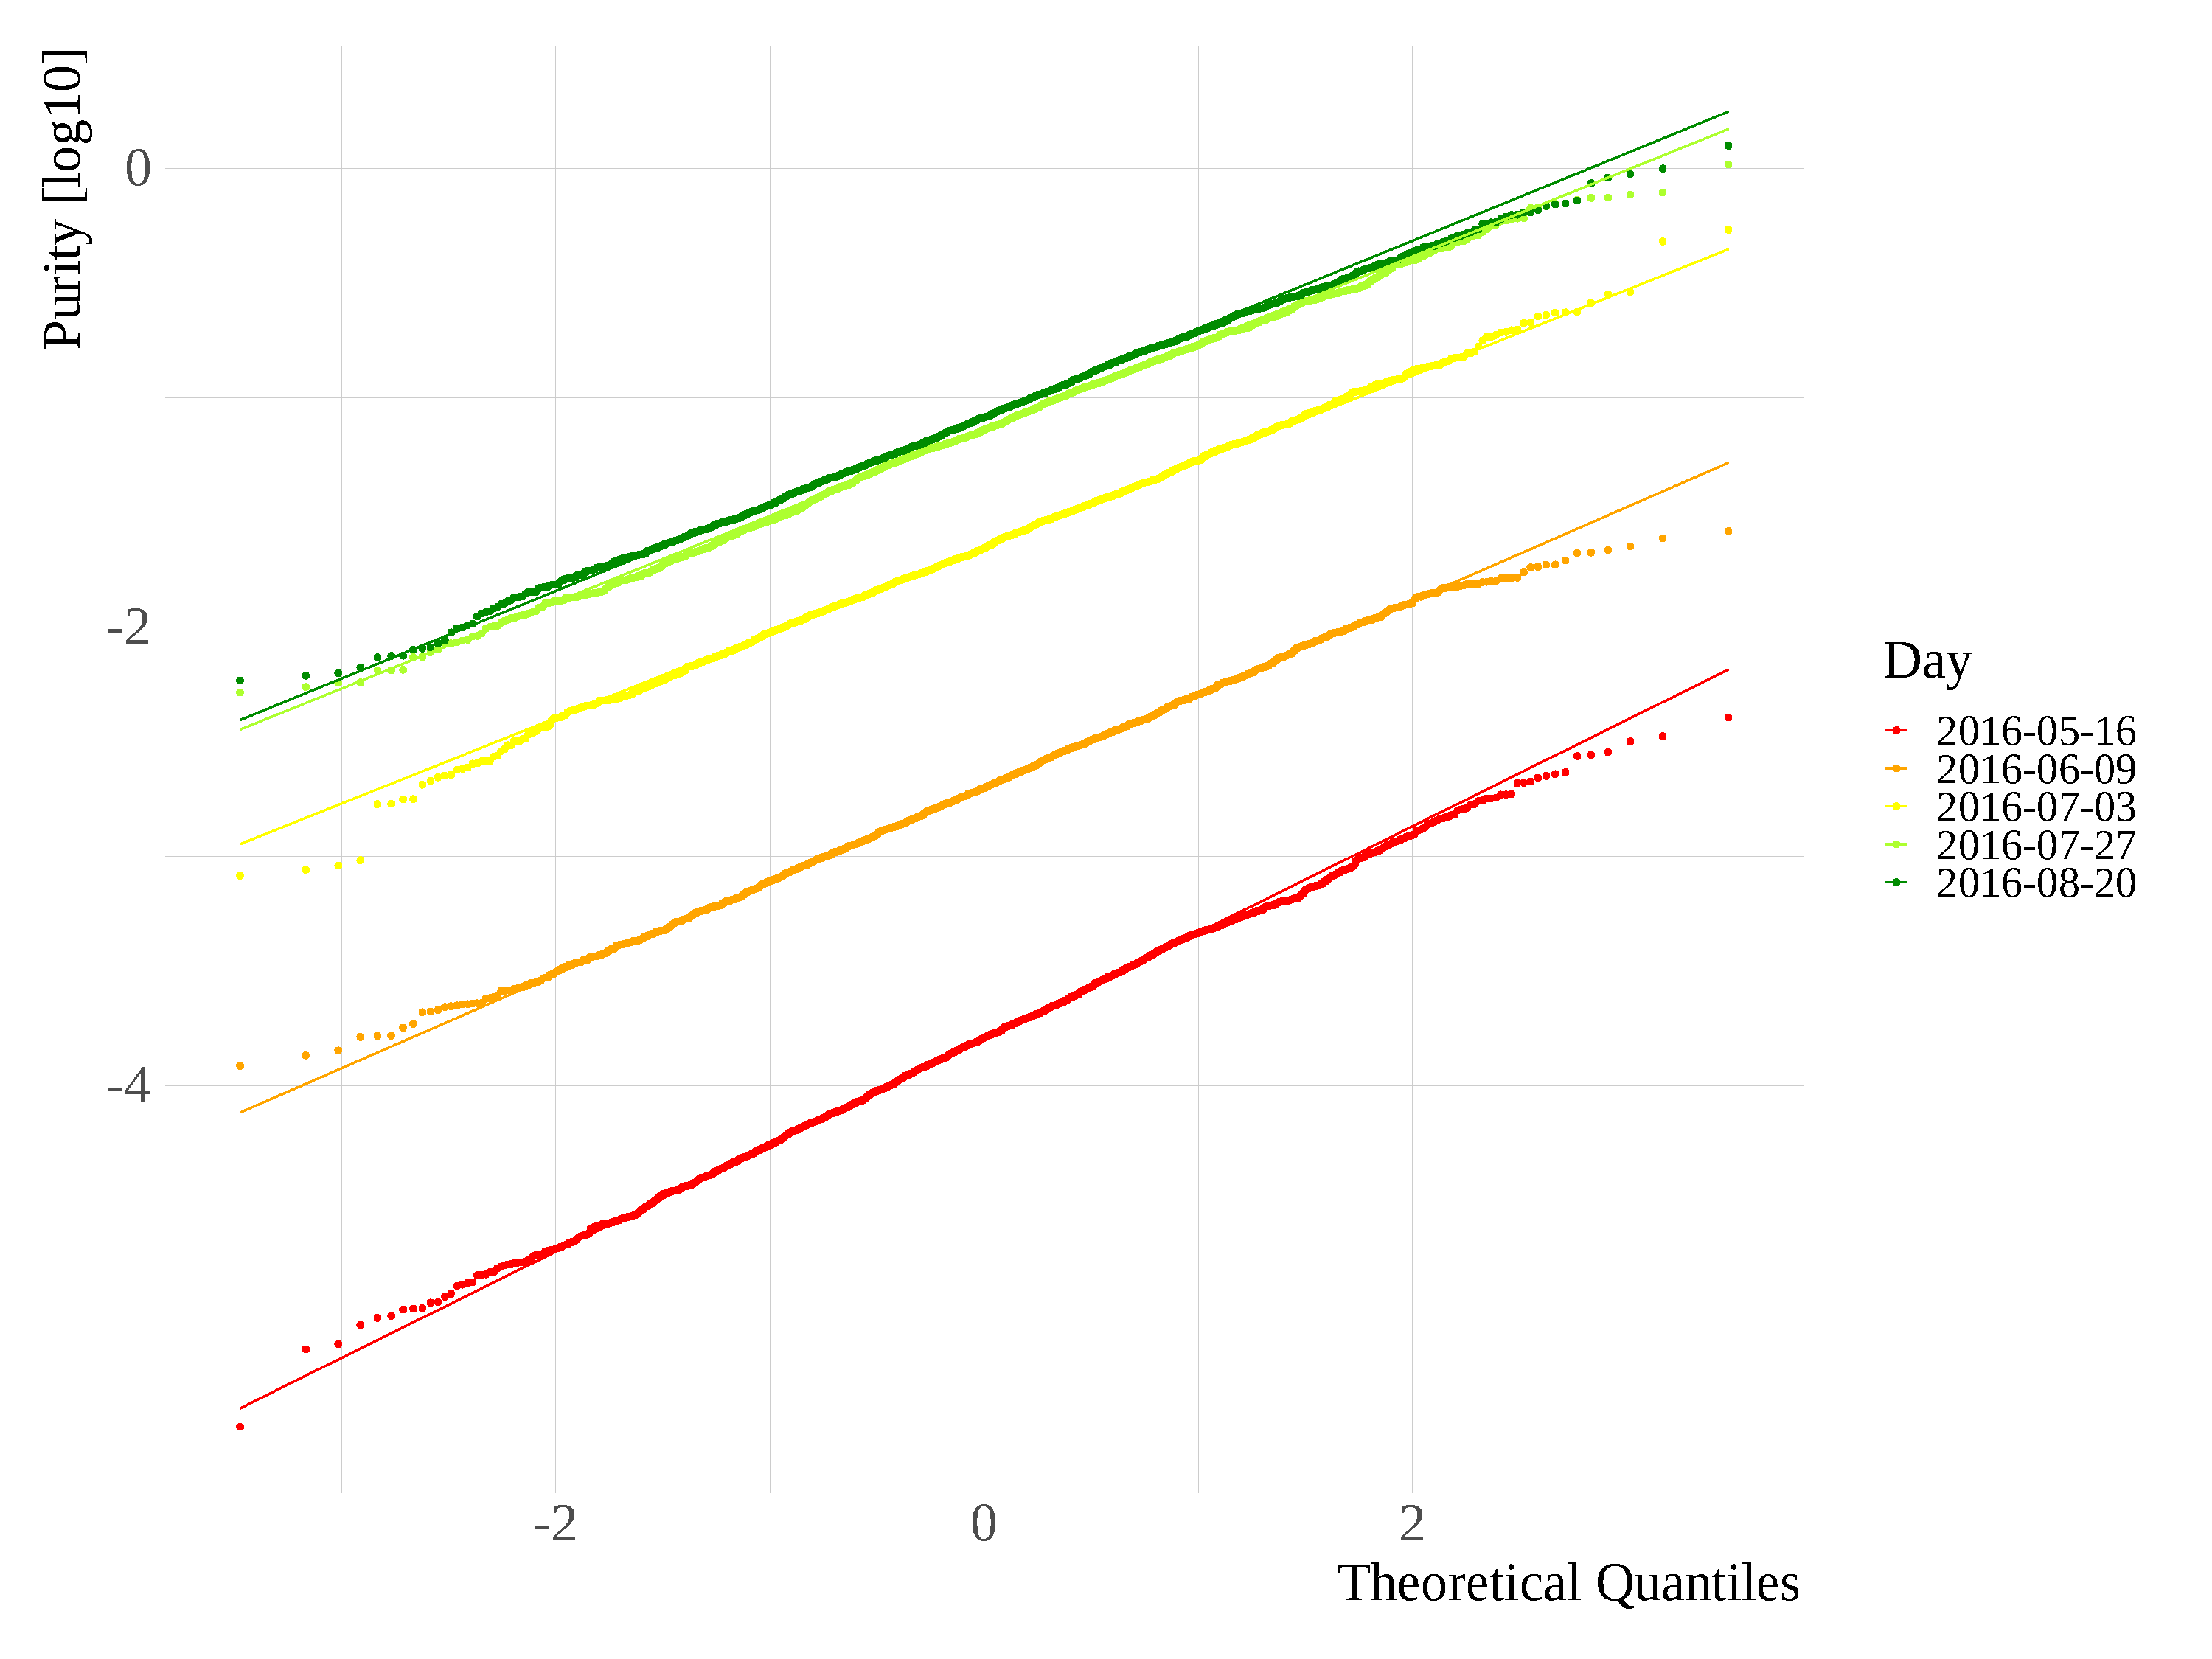
\includegraphics[width = .95\linewidth]{qqplots}}
%  \caption{Descriptive analysis of the logarithm purity values for each image}
%  \label{fig:desc_analysis}
%\end{figure}

% \begin{table}[hbt]
%   \centering
%   \caption{$p$-values from Shapiro-Wilk Test for Soybeans 231}
%   \label{tab:pvalues_purities_sb231}
%   \begin{tabular}{lrrrrr}
%     \toprule
%     \textbf{Day} & \textbf{16 May} & \textbf{09 June} & \textbf{03 July} & \textbf{27 July} & \textbf{20 Aug.}\\
%                  & \textbf{2016} & \textbf{2016} & \textbf{2016} & \textbf{2016} & \textbf{2016}\\\midrule

%     \textbf{$p$-value} & 0.4963 & 0.0650 & 0.3494 & 0.0585 & 0.3919\\
%     \bottomrule
%   \end{tabular}
% \end{table}

% \begin{table}[hbt]
%   \centering
%   \caption{$p$-values from Shapiro-Wilk Test for Canola 43}
%   \label{tab:pvalues_purities_sb231}
%   \begin{tabular}{lrrrrr}
%     \toprule
%     \textbf{Day} & \textbf{16 May} & \textbf{09 June} & \textbf{03 July} & \textbf{27 July} & \textbf{20 Aug.}\\
%                  & \textbf{2016} & \textbf{2016} & \textbf{2016} & \textbf{2016} & \textbf{2016}\\\midrule

%     \textbf{$p$-value} & 0.1143 & 0.7359 & 0.5855 & $2.6\times 10^{-16}$ & $2.6\times 10^{-16}$\\
%     \bottomrule
%   \end{tabular}
% \end{table}

% \begin{table}[hbt]
%   \centering
%   \caption{$p$-values from Shapiro-Wilk Test for Wheat 104}
%   \label{tab:pvalues_purities_sb231}
%   \begin{tabular}{lrrrrr}
%     \toprule
%     \textbf{Day} & \textbf{16 May} & \textbf{09 June} & \textbf{03 July} & \textbf{27 July} & \textbf{20 Aug.}\\
%                  & \textbf{2016} & \textbf{2016} & \textbf{2016} & \textbf{2016} & \textbf{2016}\\\midrule

%     \textbf{$p$-value} & 0.8189 & 0.9042 & 0.0025 & 0.3929 & 0.0544\\
%     \bottomrule
%   \end{tabular}
% \end{table}

% \begin{table}[hbt]
%   \centering
%   \caption{$p$-values from Shapiro-Wilk Test for Oats 102}
%   \label{tab:pvalues_purities_sb231}
%   \begin{tabular}{lrrrrr}
%     \toprule
%     \textbf{Day} & \textbf{16 May} & \textbf{09 June} & \textbf{03 July} & \textbf{27 July} & \textbf{20 Aug.}\\
%                  & \textbf{2016} & \textbf{2016} & \textbf{2016} & \textbf{2016} & \textbf{2016}\\\midrule

%     \textbf{$p$-value} & 0.4928 & $5.24\times 10^{-8}$ & 0.5263 & 0.0484 & 0.9694\\
%     \bottomrule
%   \end{tabular}
% \end{table}


\section{Data analysis}

Descriptive statistics

Fitting distributions

Separability tests



\begin{figure}[hbt]
\centering
\subcaptionbox{16 May 2016}{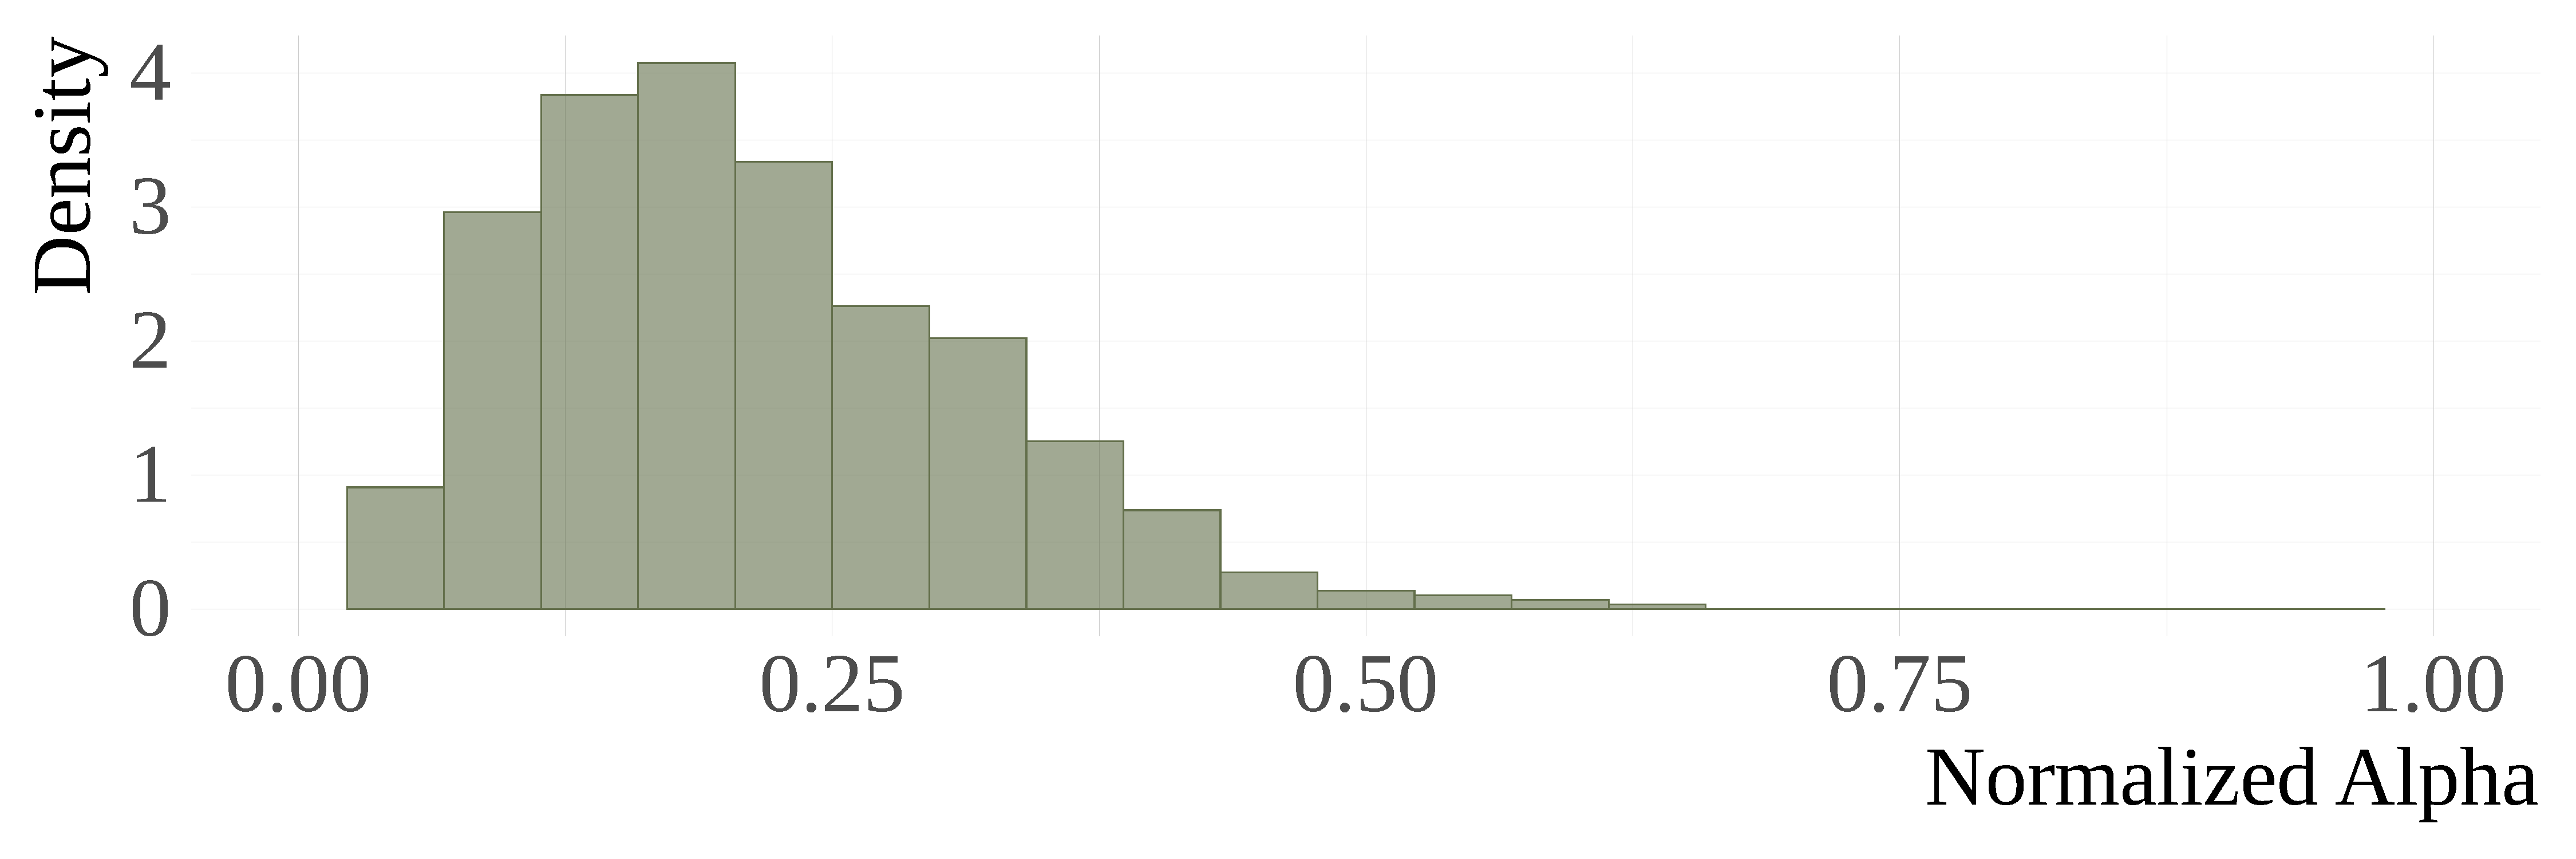
\includegraphics[width = \linewidth]{alpha_sb231_1}}
\subcaptionbox{09 June 2016}{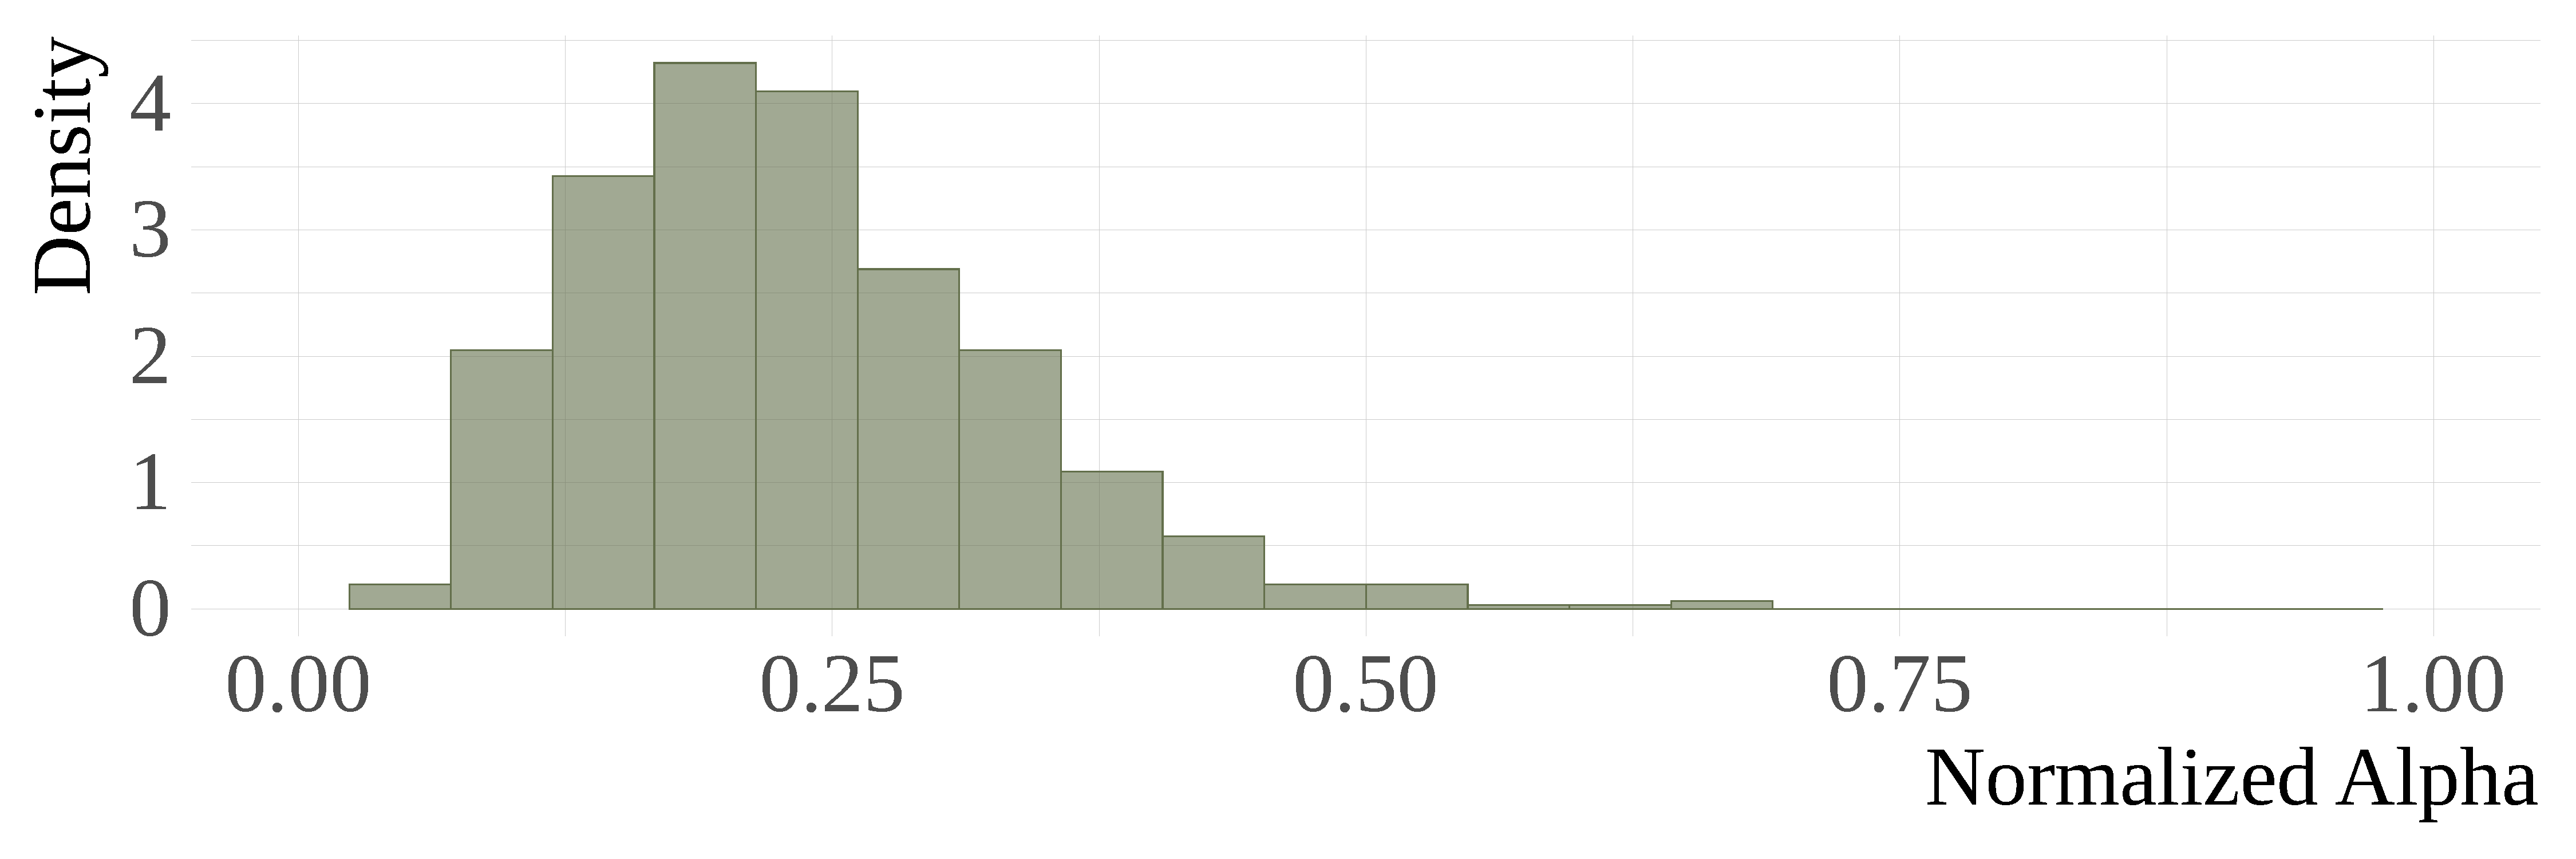
\includegraphics[width = \linewidth]{alpha_sb231_2}}
\subcaptionbox{03 July 2016}{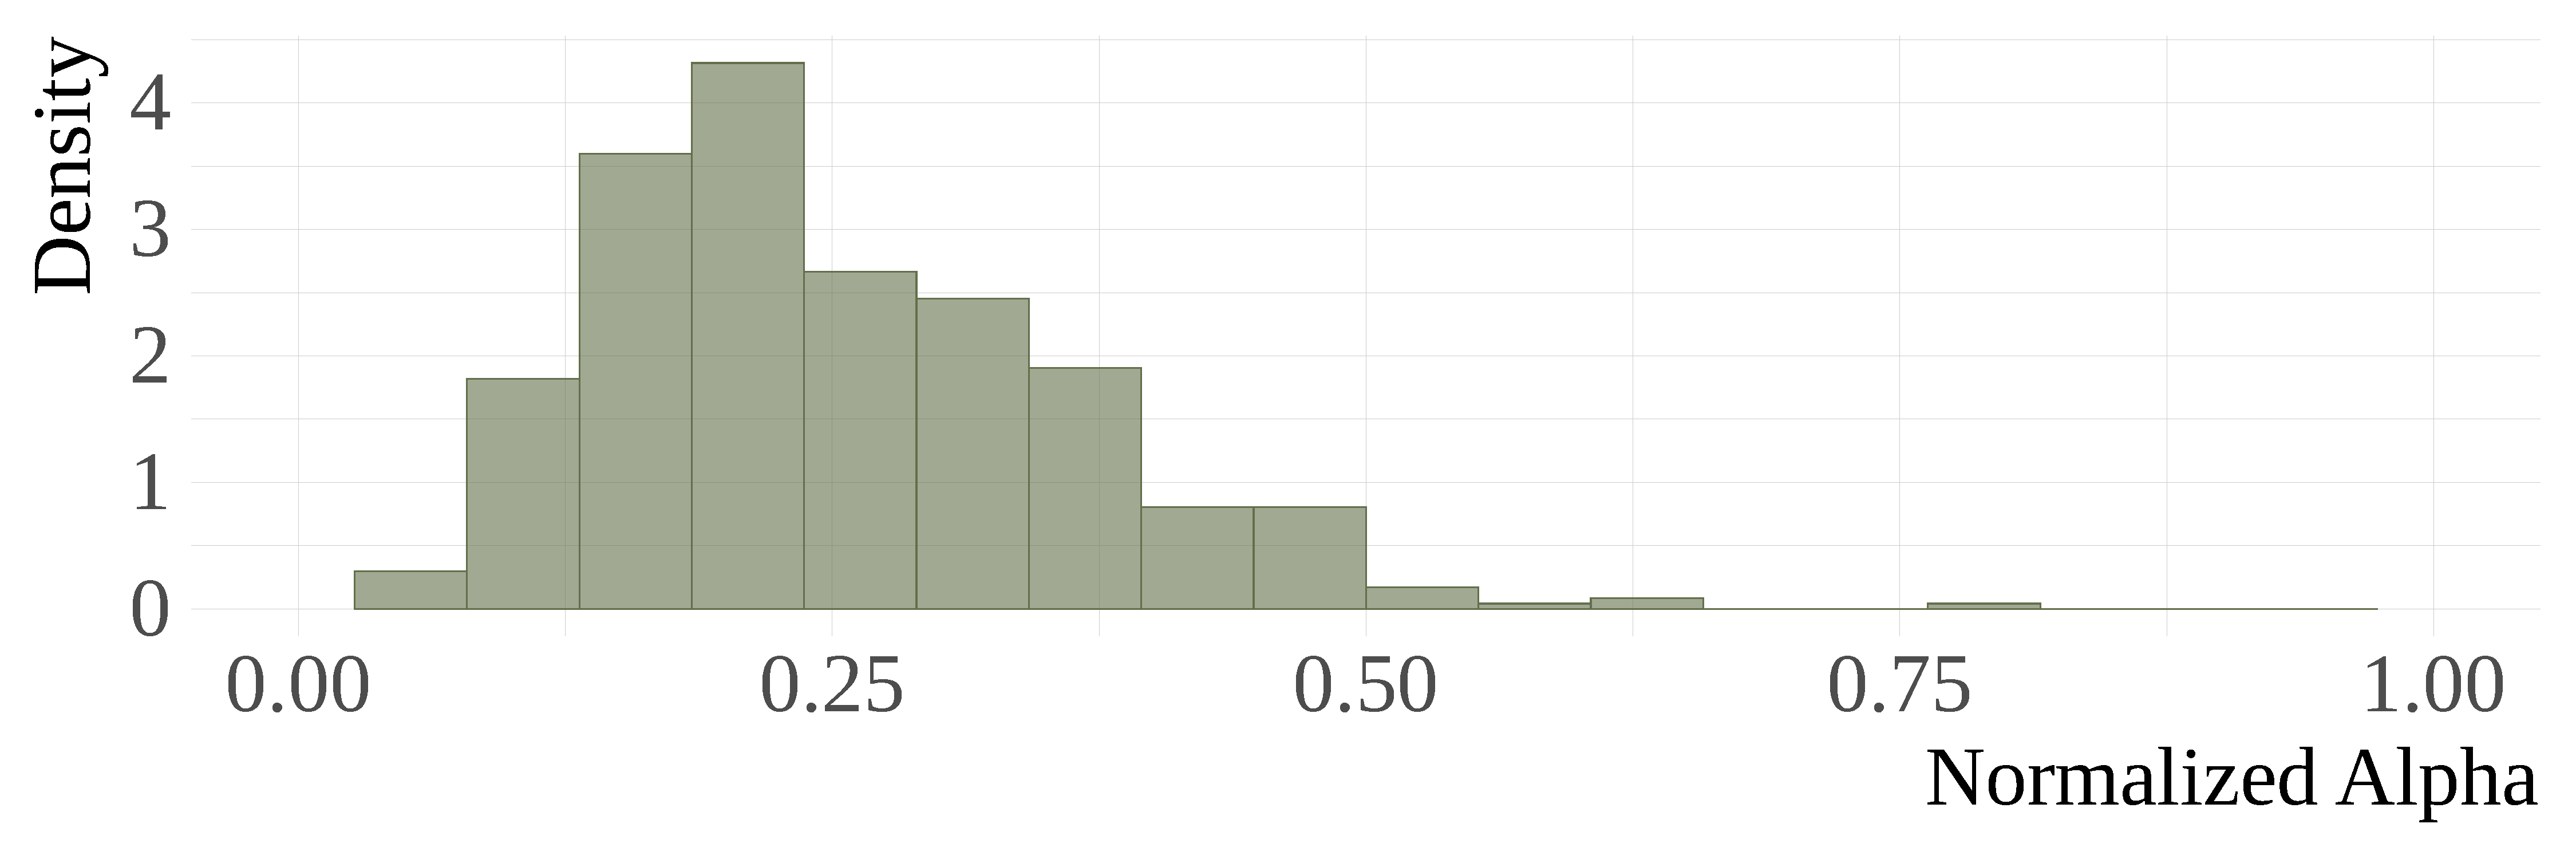
\includegraphics[width = \linewidth]{alpha_sb231_3}}
\subcaptionbox{27 July 2016}{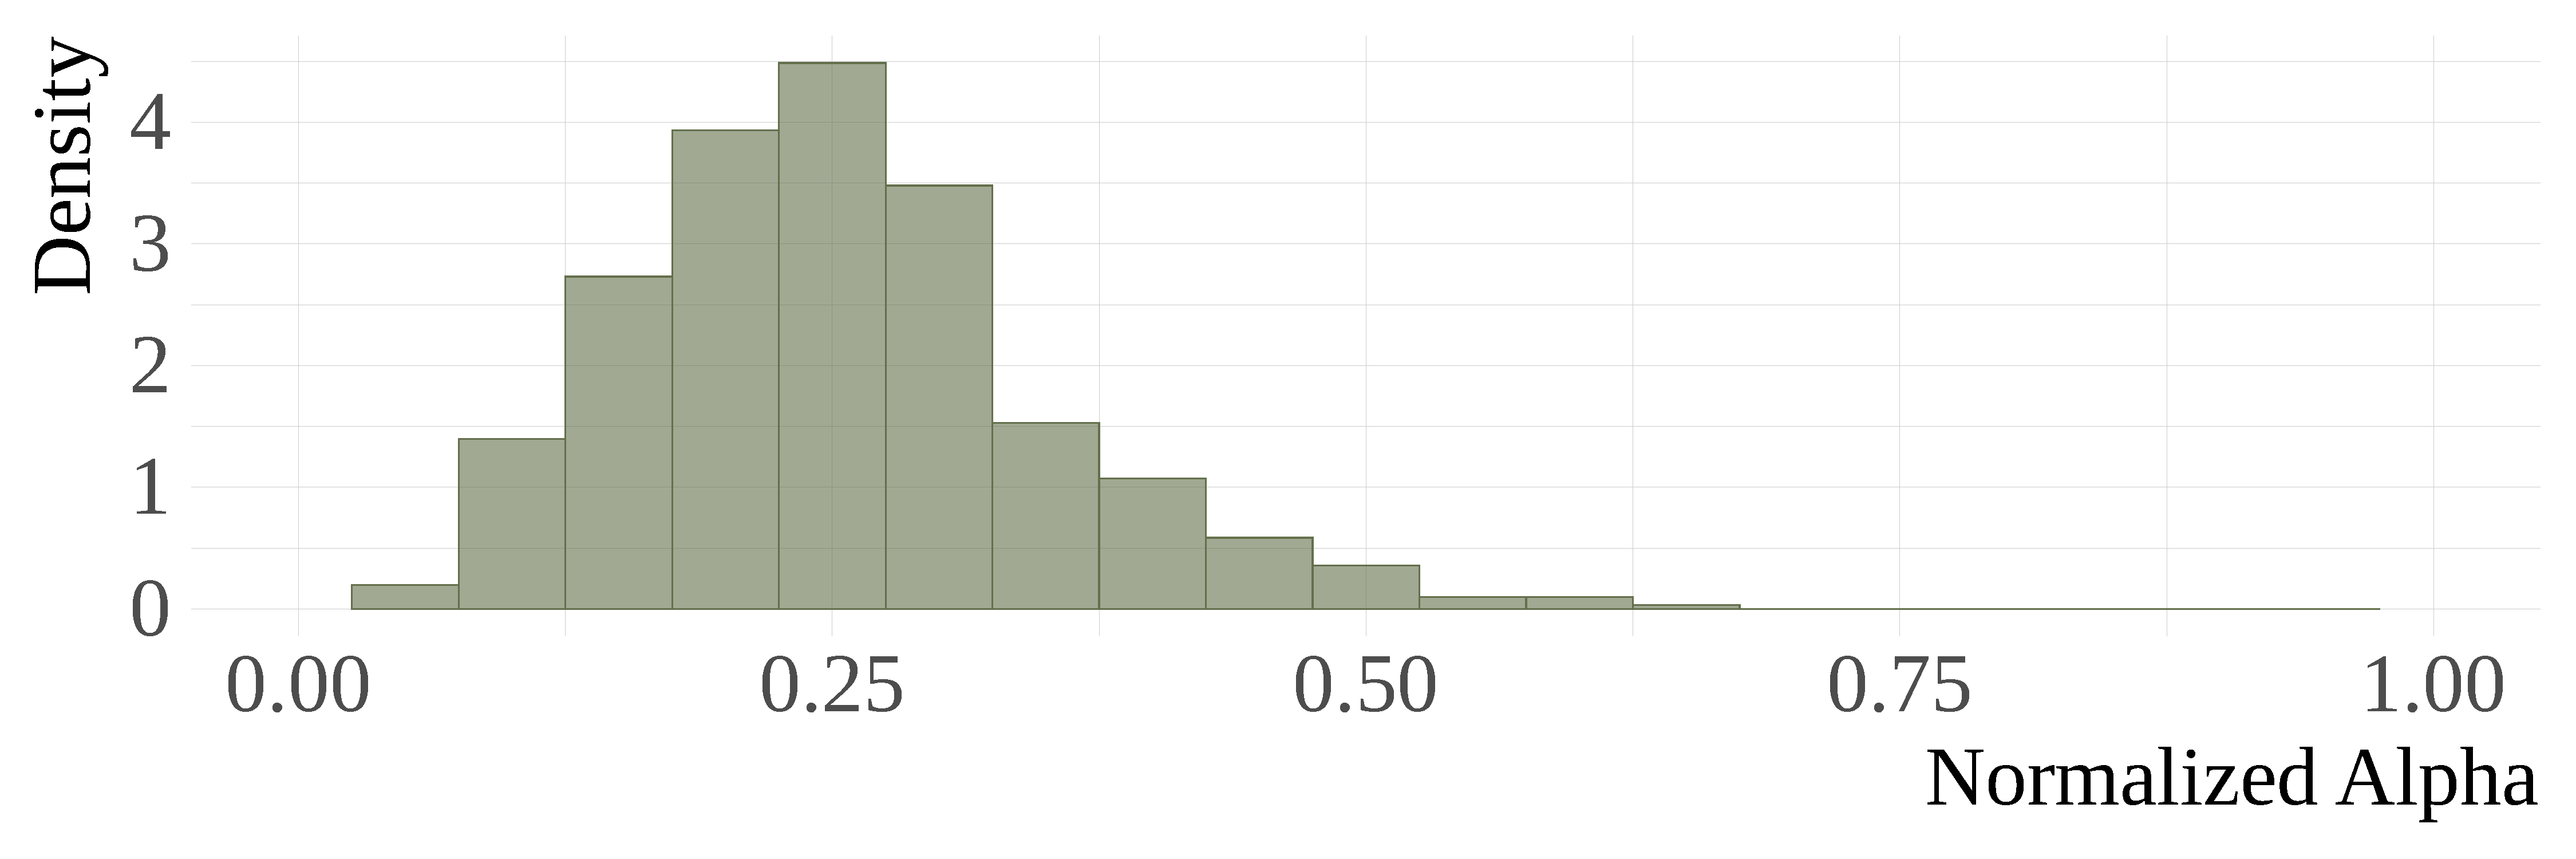
\includegraphics[width = \linewidth]{alpha_sb231_4}}
\subcaptionbox{20 August 2016}{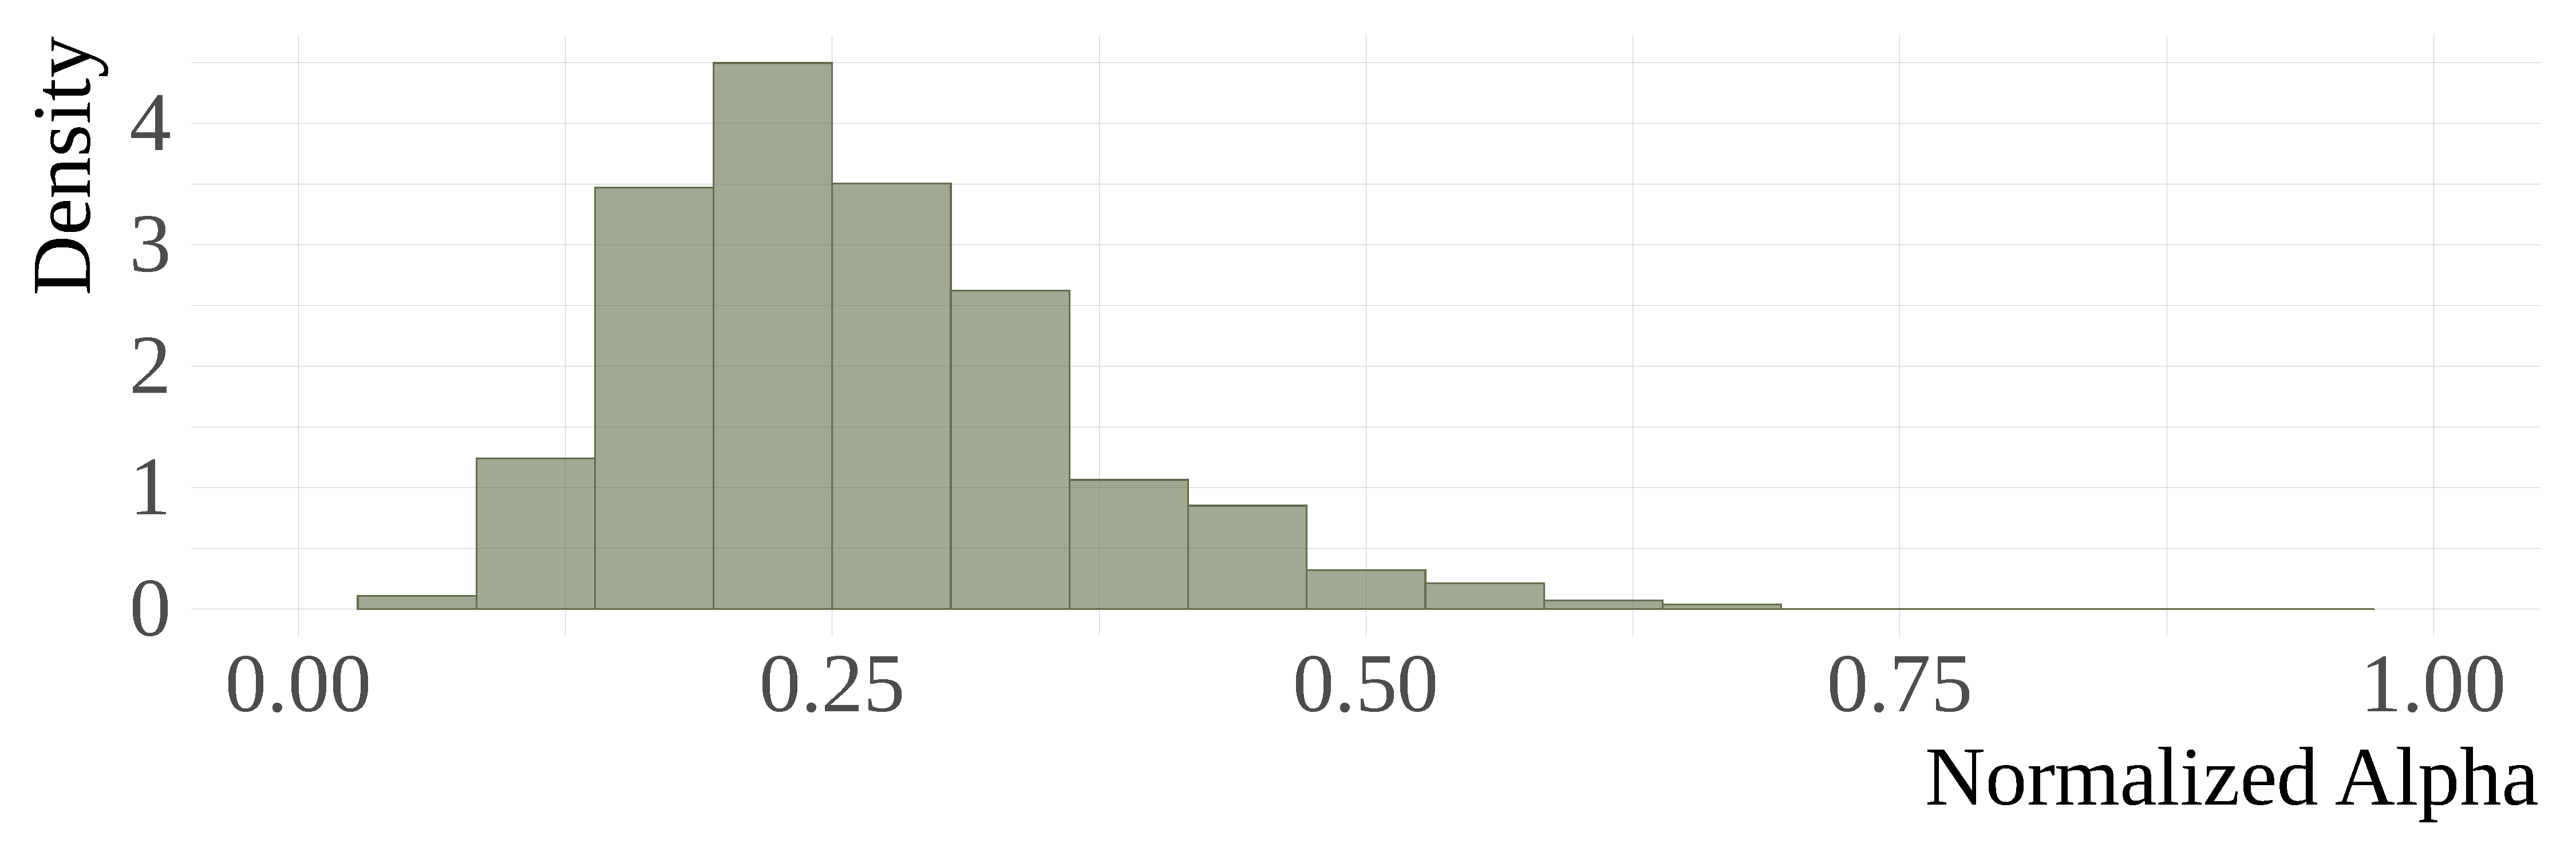
\includegraphics[width = \linewidth]{alpha_sb231_5}}
\caption{Histograms of the geodesic distances between trihedral and the pixels from Soybeans 231 most similar to trihedral}
\label{fig:histograms_alpha_sb231}
\end{figure}

\begin{table}[hbt]
  \centering
  \caption{$p$-values from Komolgorov-Smirnov Test for normalized from Soybeans 231}
  \label{tab:pvalues_alpha_sb231}
  \begin{tabular}{lrrrrr}
    \toprule
    \textbf{Day} & \textbf{16 May} & \textbf{09 June} & \textbf{03 July} & \textbf{27 July} & \textbf{20 Aug.}\\ 
                 & \textbf{2016} & \textbf{2016} & \textbf{2016} & \textbf{2016} & \textbf{2016}\\\midrule
    \textbf{Sample size} & 1285 & 656 & 449 & 615 & 508\\
    \textbf{$p$-value} & 0.7746 & 0.5734 & 0.3137 & 0.2392 & 0.4158\\
    \bottomrule
  \end{tabular}
\end{table}

\begin{figure}[hbt]
\centering
\subcaptionbox{16 May 2016}{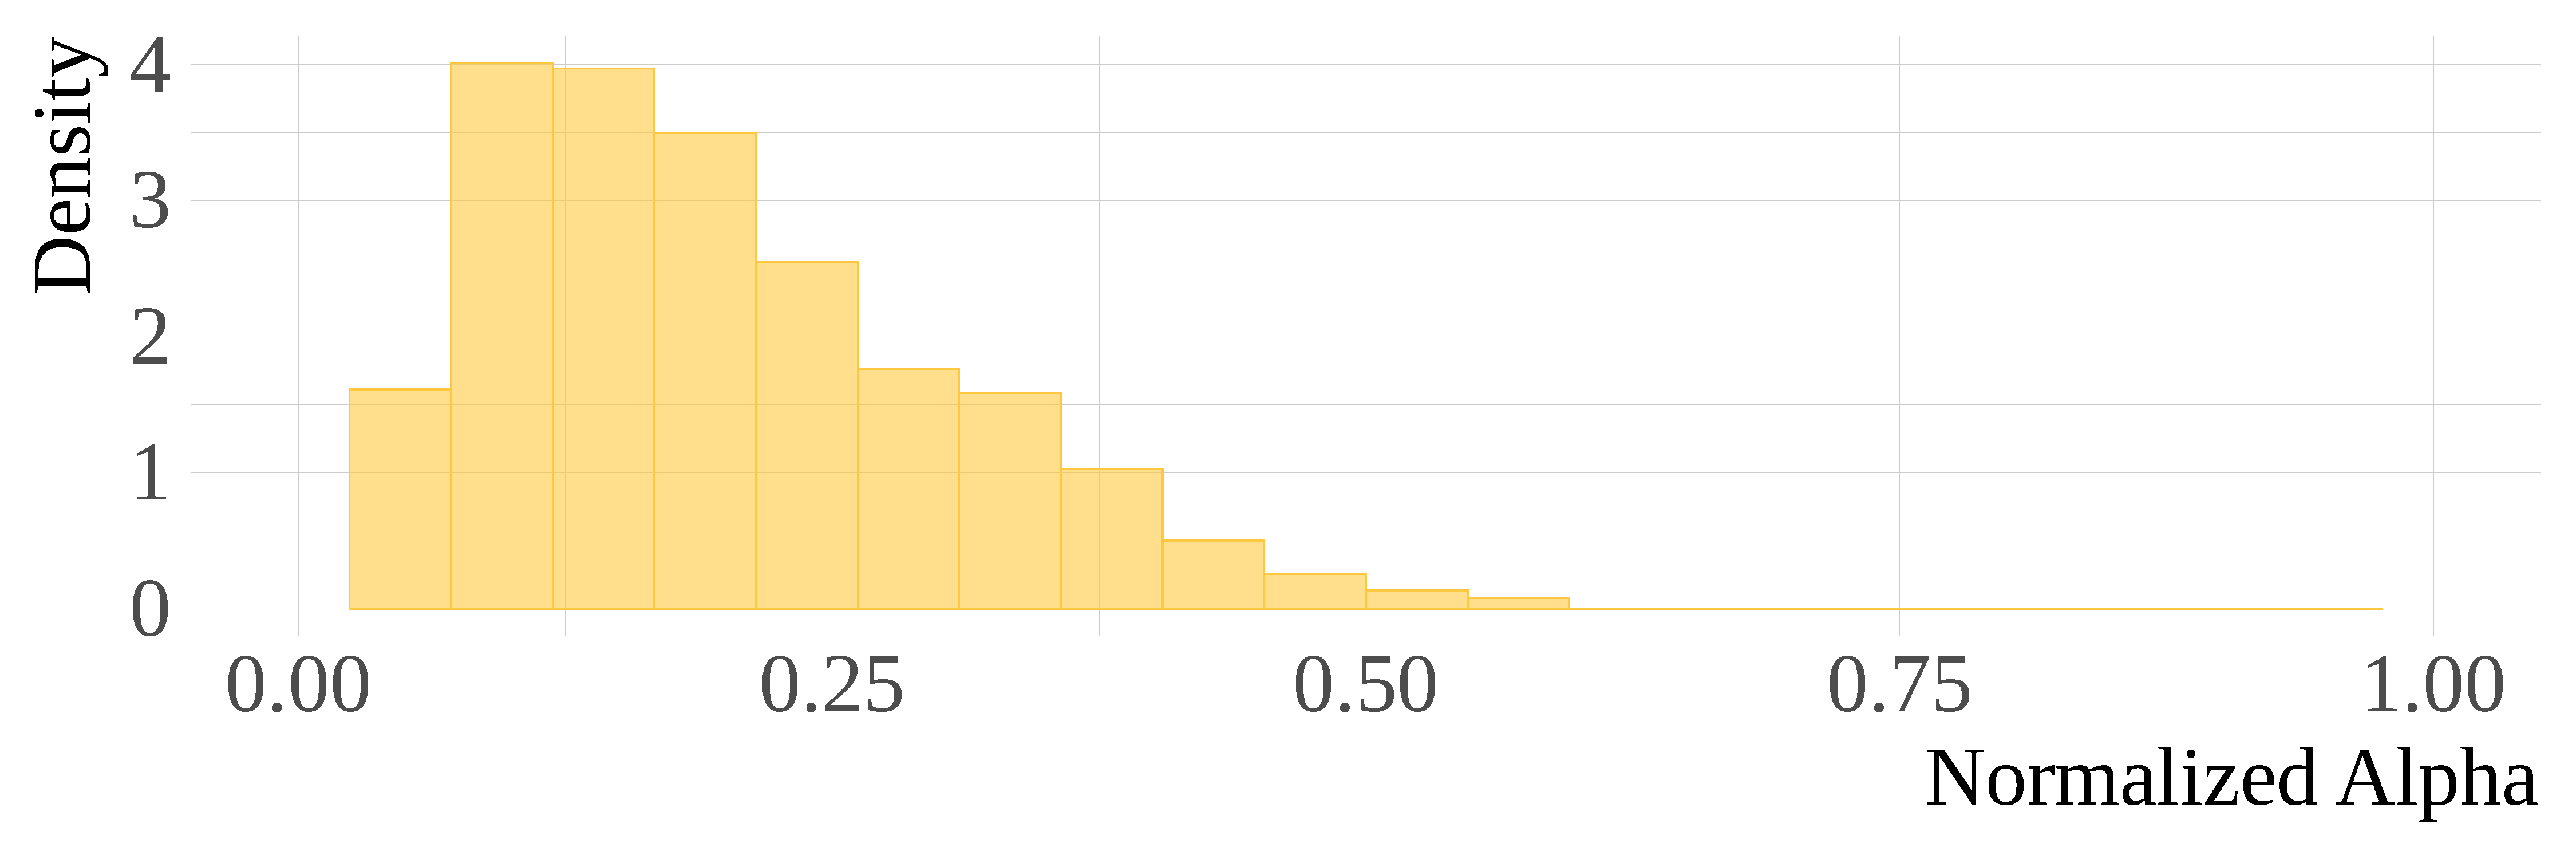
\includegraphics[width = \linewidth]{alpha_cn43_1}}
\subcaptionbox{09 June 2016}{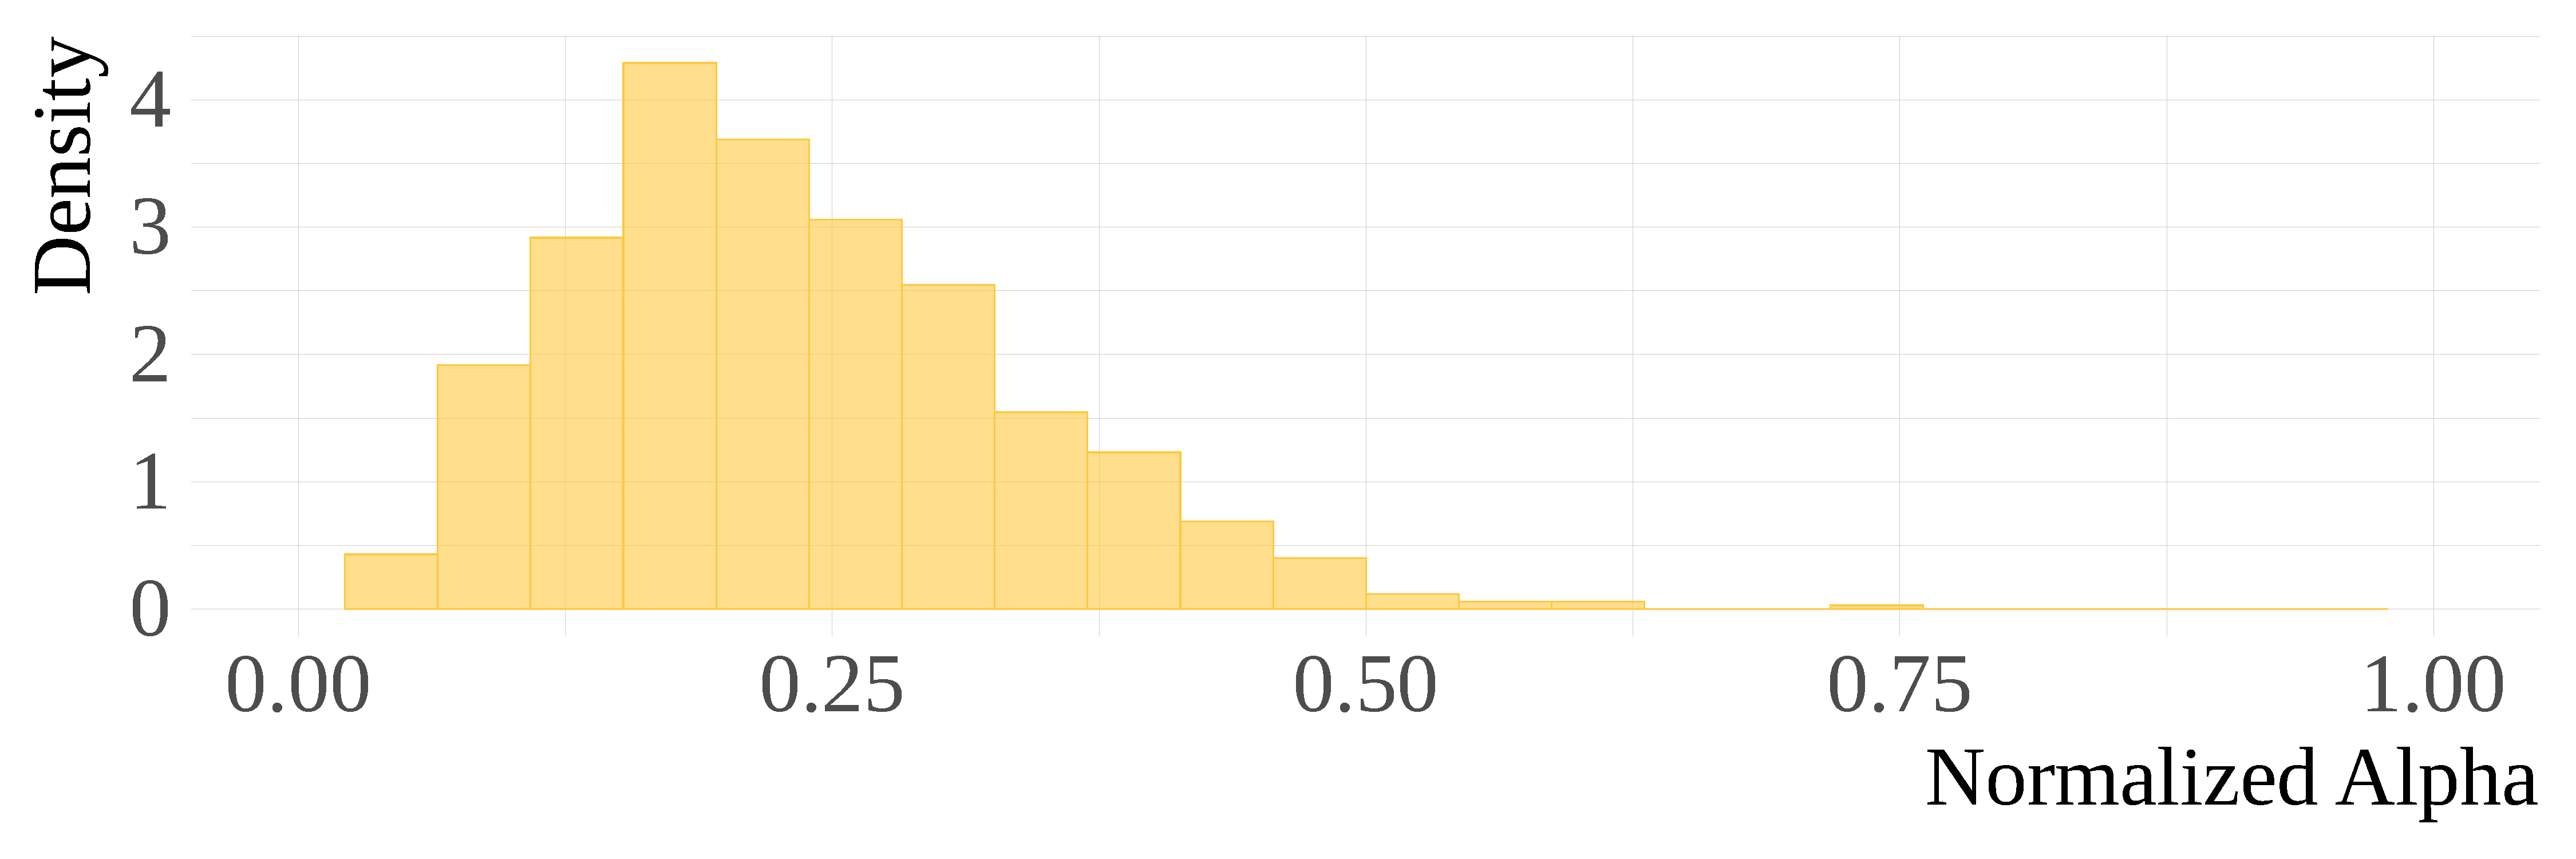
\includegraphics[width = \linewidth]{alpha_cn43_2}}
\subcaptionbox{03 July 2016}{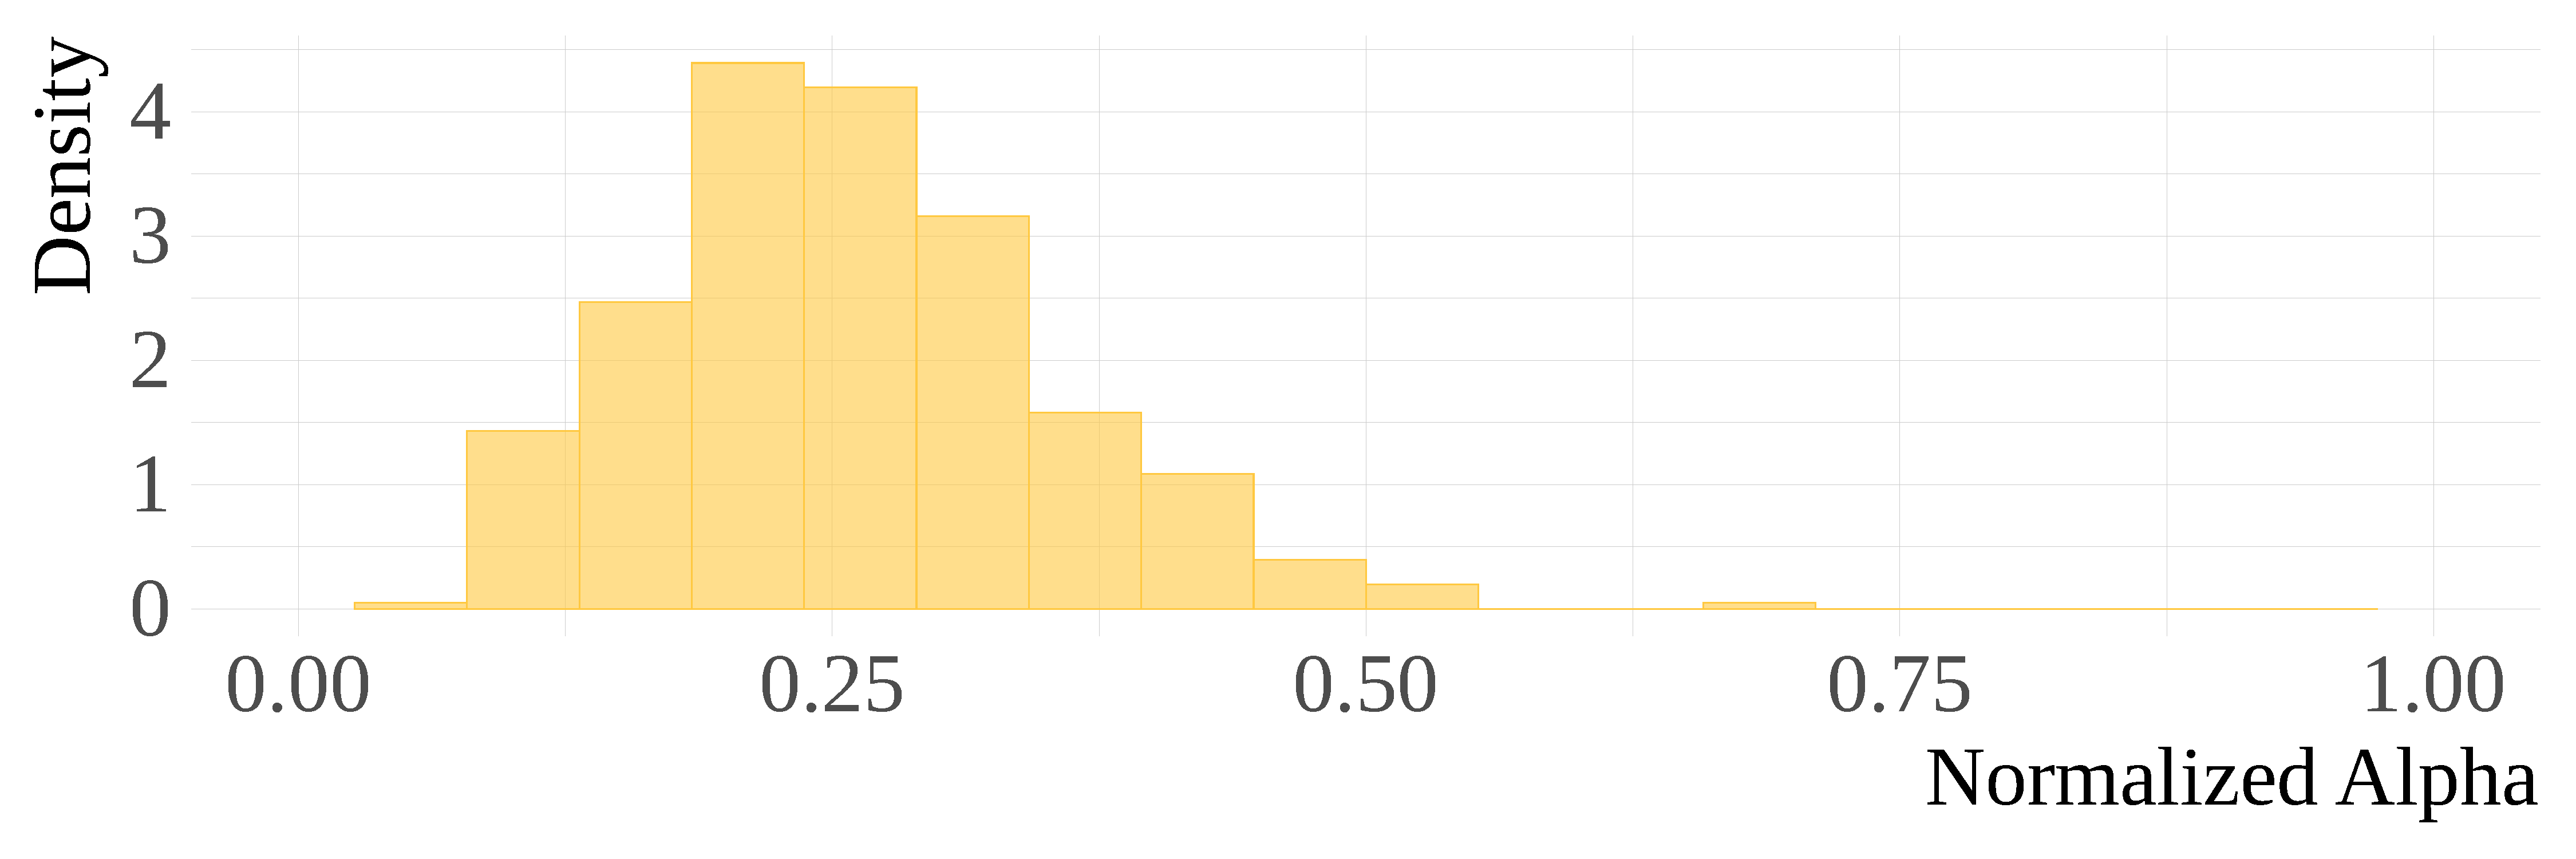
\includegraphics[width = \linewidth]{alpha_cn43_3}}
\subcaptionbox{27 July 2016}{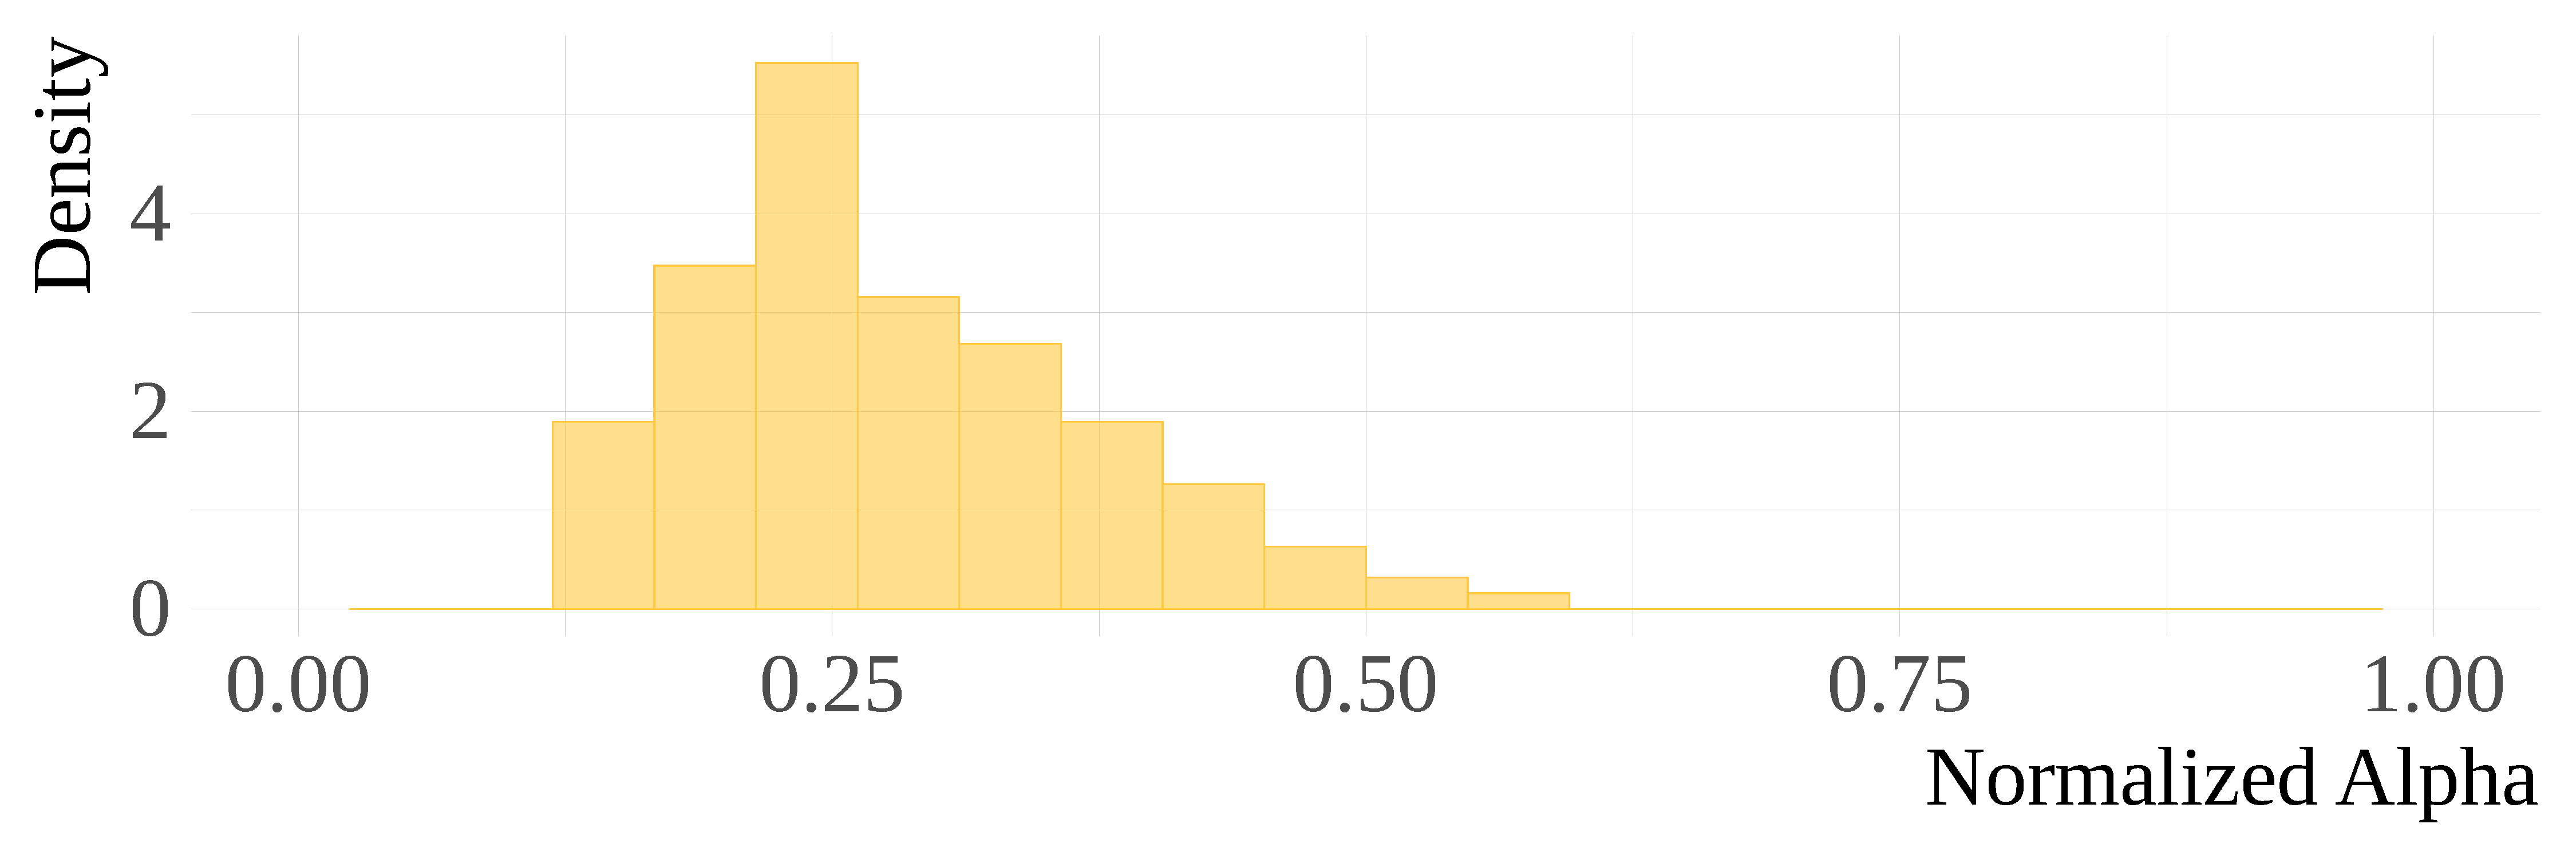
\includegraphics[width = \linewidth]{alpha_cn43_4}}
\subcaptionbox{20 August 2016}{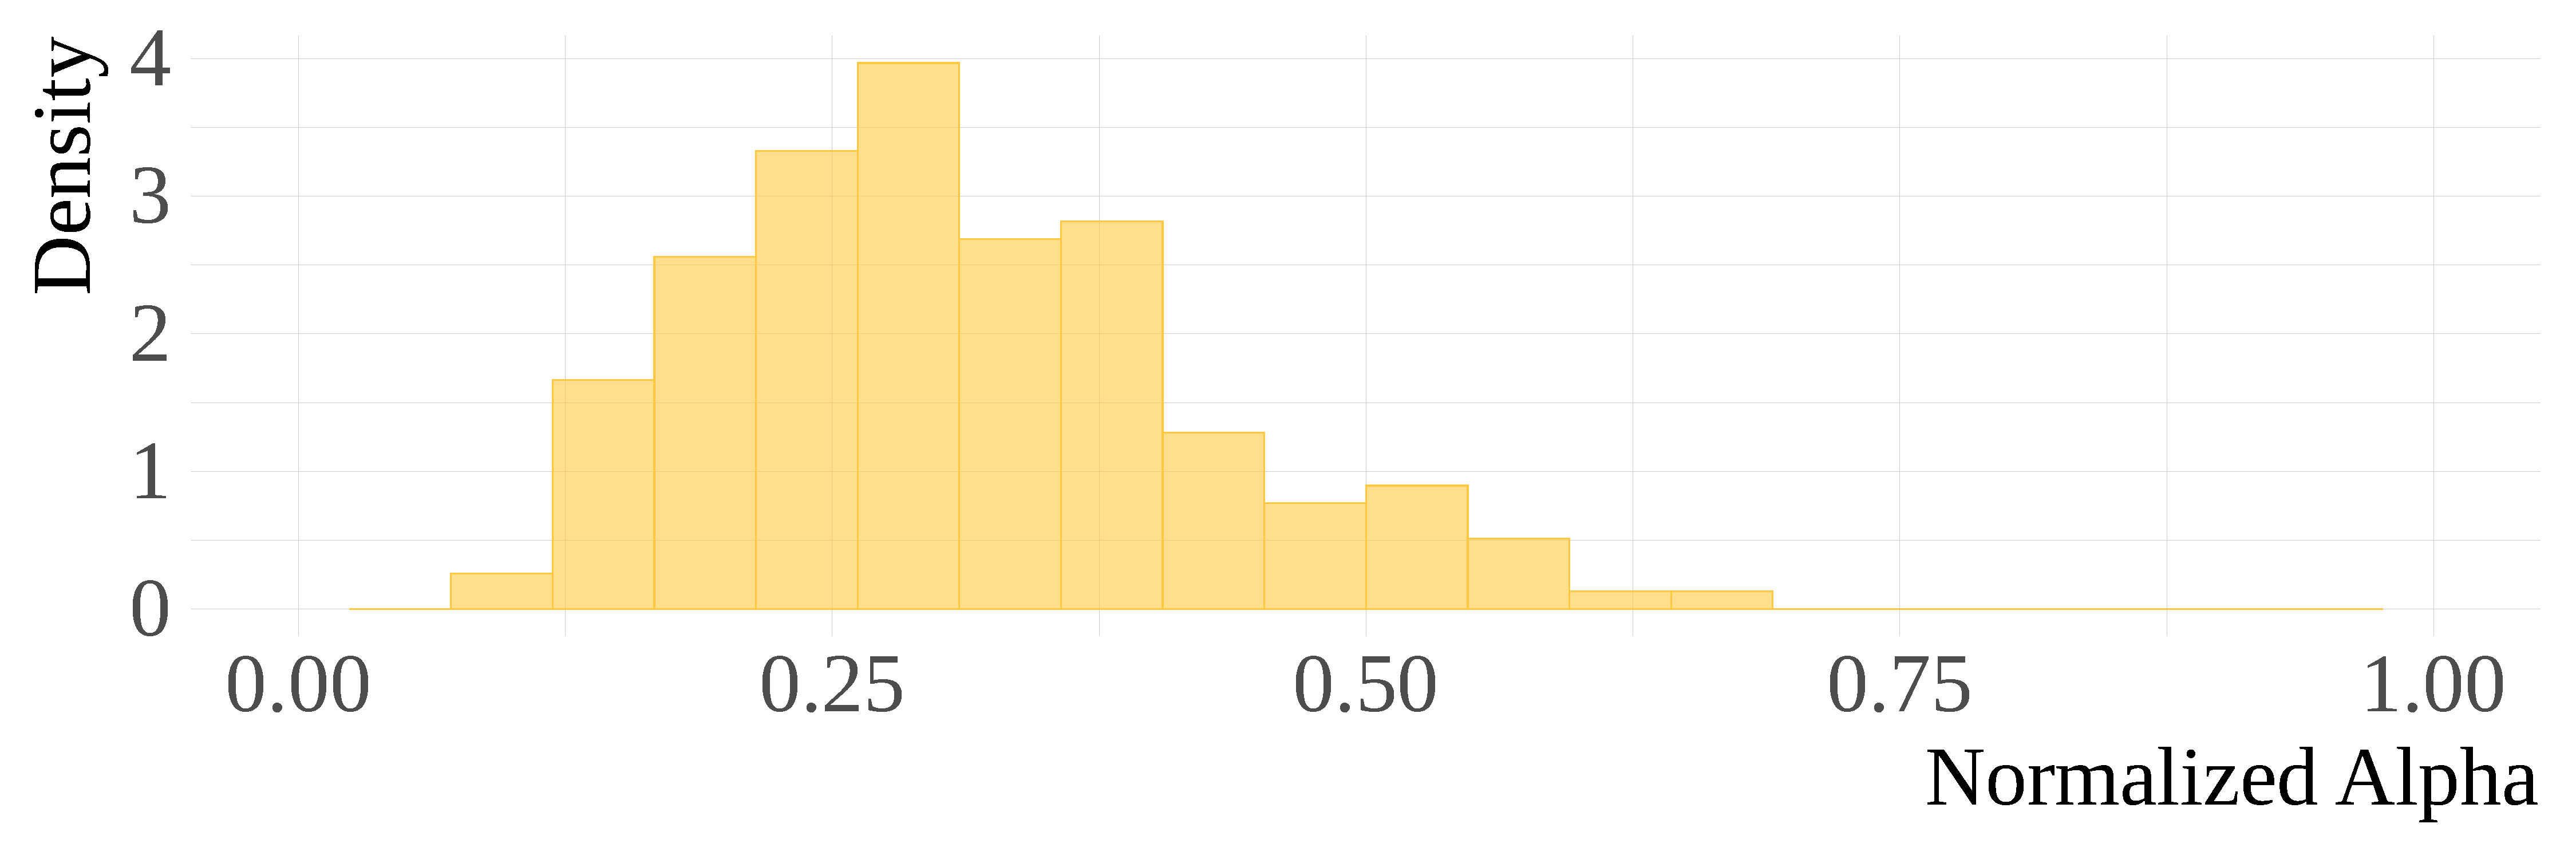
\includegraphics[width = \linewidth]{alpha_cn43_5}}
\caption{Histograms of the geodesic distances between trihedral and the pixels from Canola 43 most similar to trihedral}
\label{fig:histograms_alpha_cn43}
\end{figure}

\begin{table}[hbt]
  \centering
  \caption{$p$-values from Komolgorov-Smirnov Test for normalized alpha from Canola 43}
  \label{tab:pvalues_alpha_cn43}
  \begin{tabular}{lrrrrr}
    \toprule
    \textbf{Day} & \textbf{16 May} & \textbf{09 June} & \textbf{03 July} & \textbf{27 July} & \textbf{20 Aug.}\\ 
                 & \textbf{2016} & \textbf{2016} & \textbf{2016} & \textbf{2016} & \textbf{2016}\\\midrule
    \textbf{Sample size} & 1549 & 804 & 385 & 133 & 164\\
    \textbf{$p$-value} & 0.2292 & 0.6397 & 0.8759 & 0.3613 & 0.8828\\
    \bottomrule
  \end{tabular}
\end{table}

\begin{figure}[hbt]
\centering
\subcaptionbox{16 May 2016}{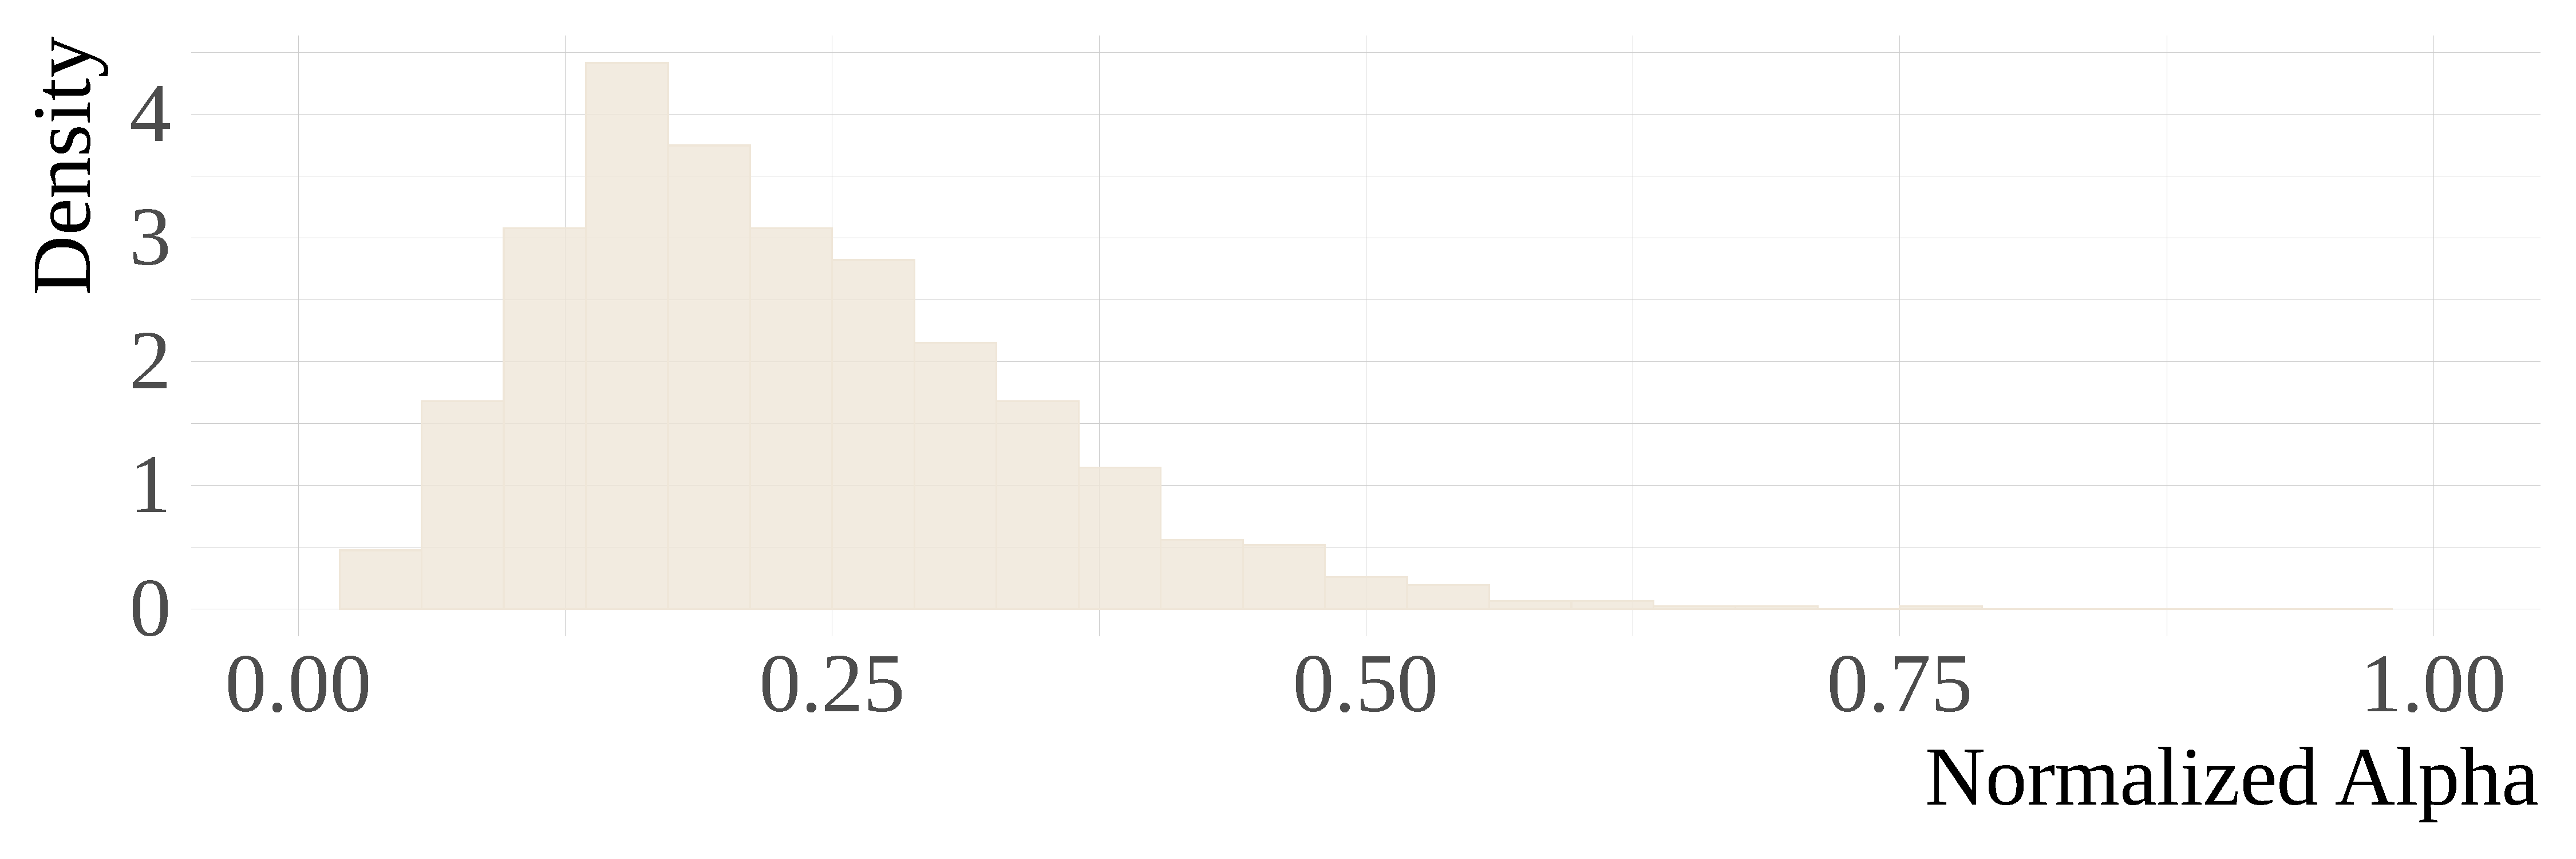
\includegraphics[width = \linewidth]{alpha_ot102_1}}
\subcaptionbox{09 June 2016}{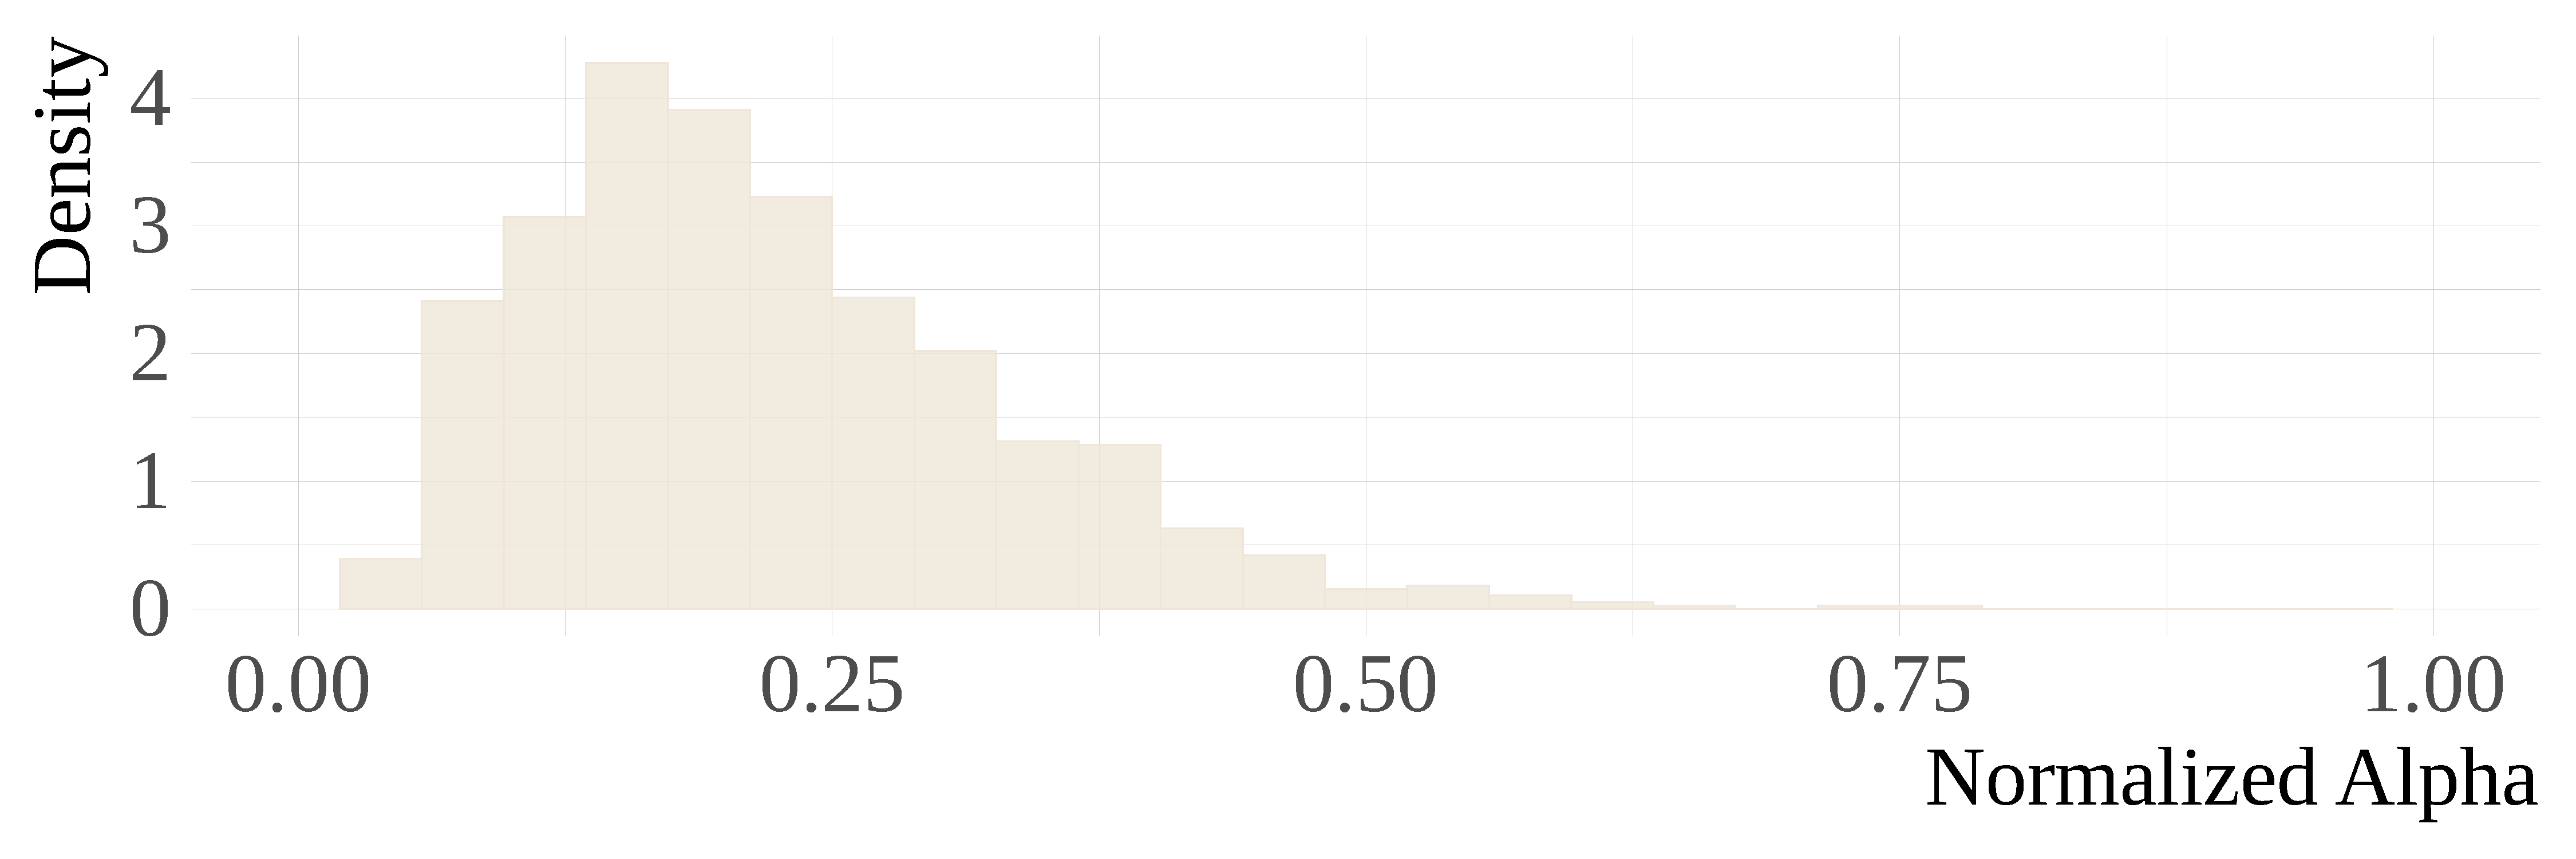
\includegraphics[width = \linewidth]{alpha_ot102_2}}
\subcaptionbox{03 July 2016}{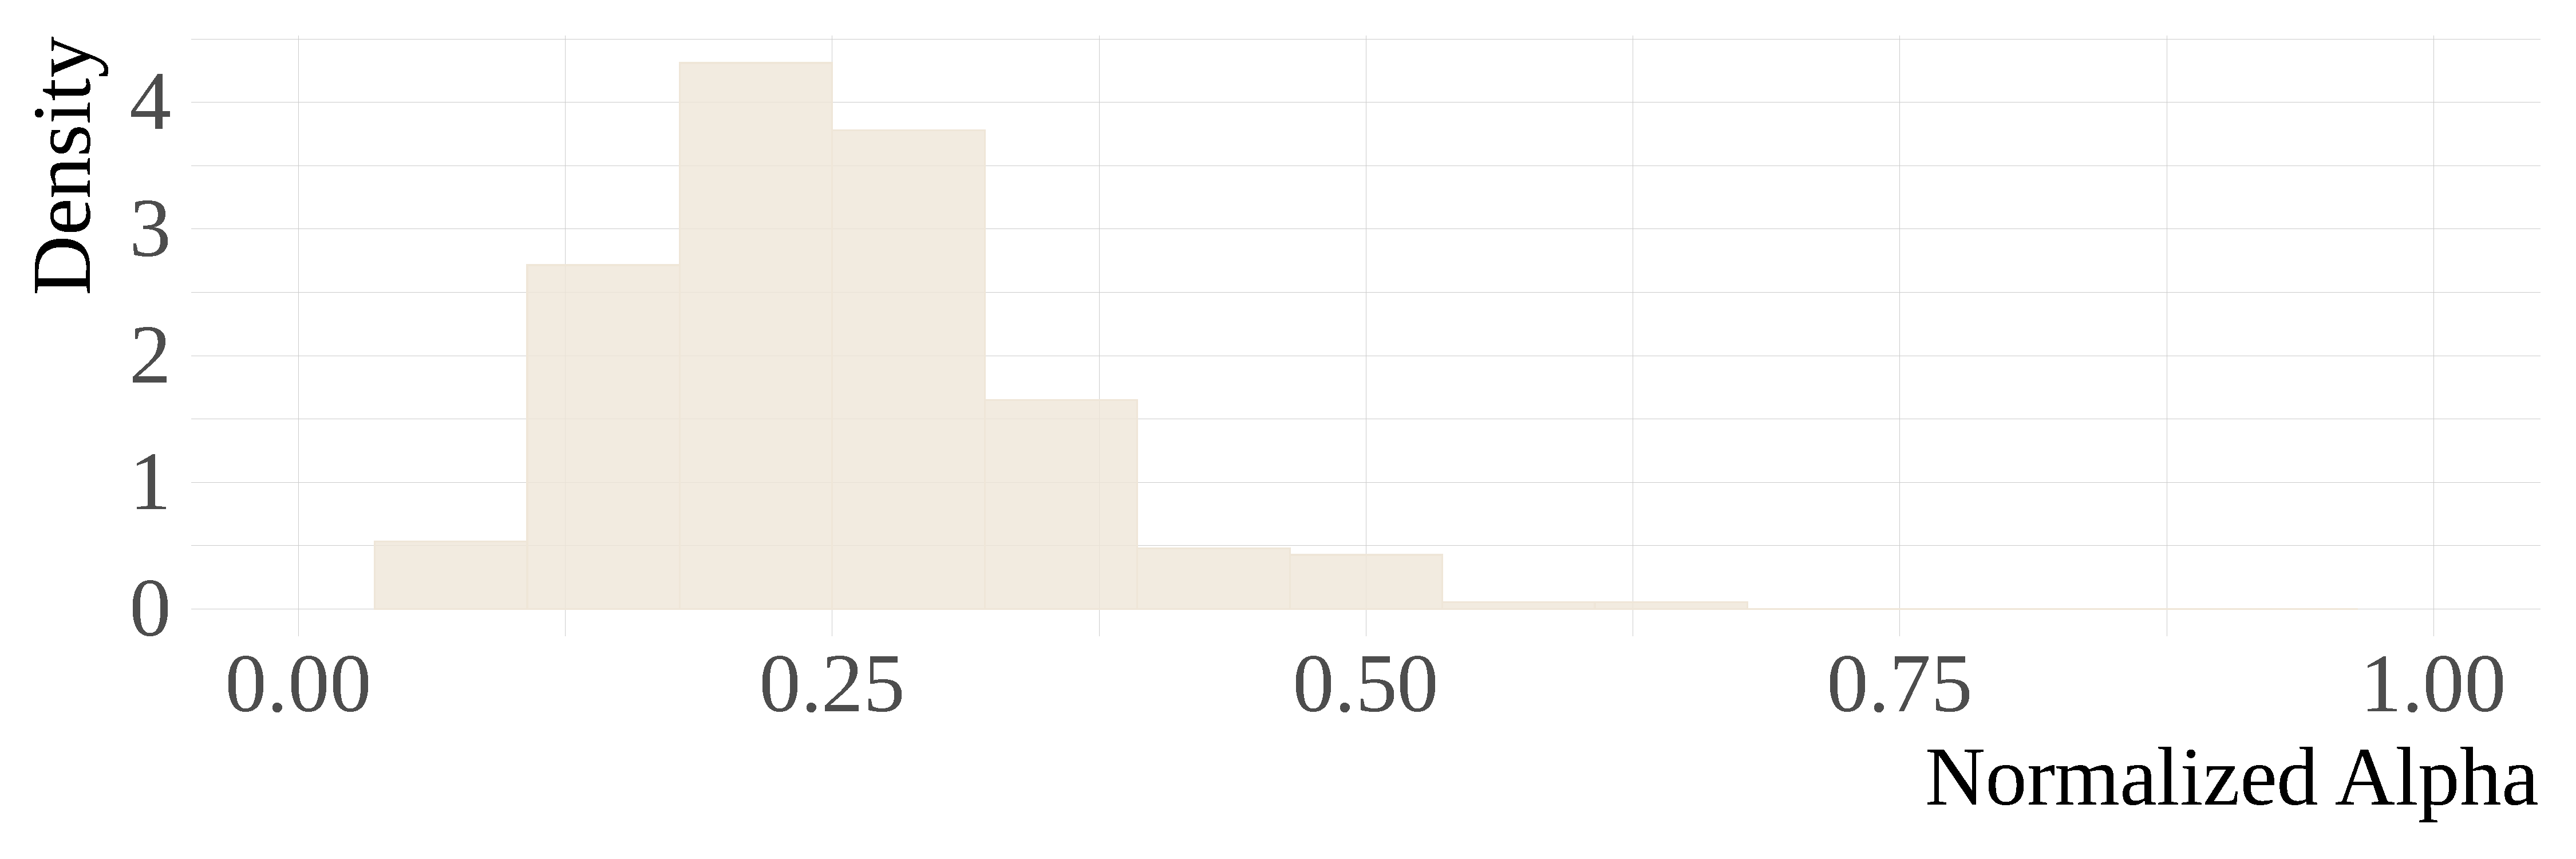
\includegraphics[width = \linewidth]{alpha_ot102_3}}
\subcaptionbox{27 July 2016}{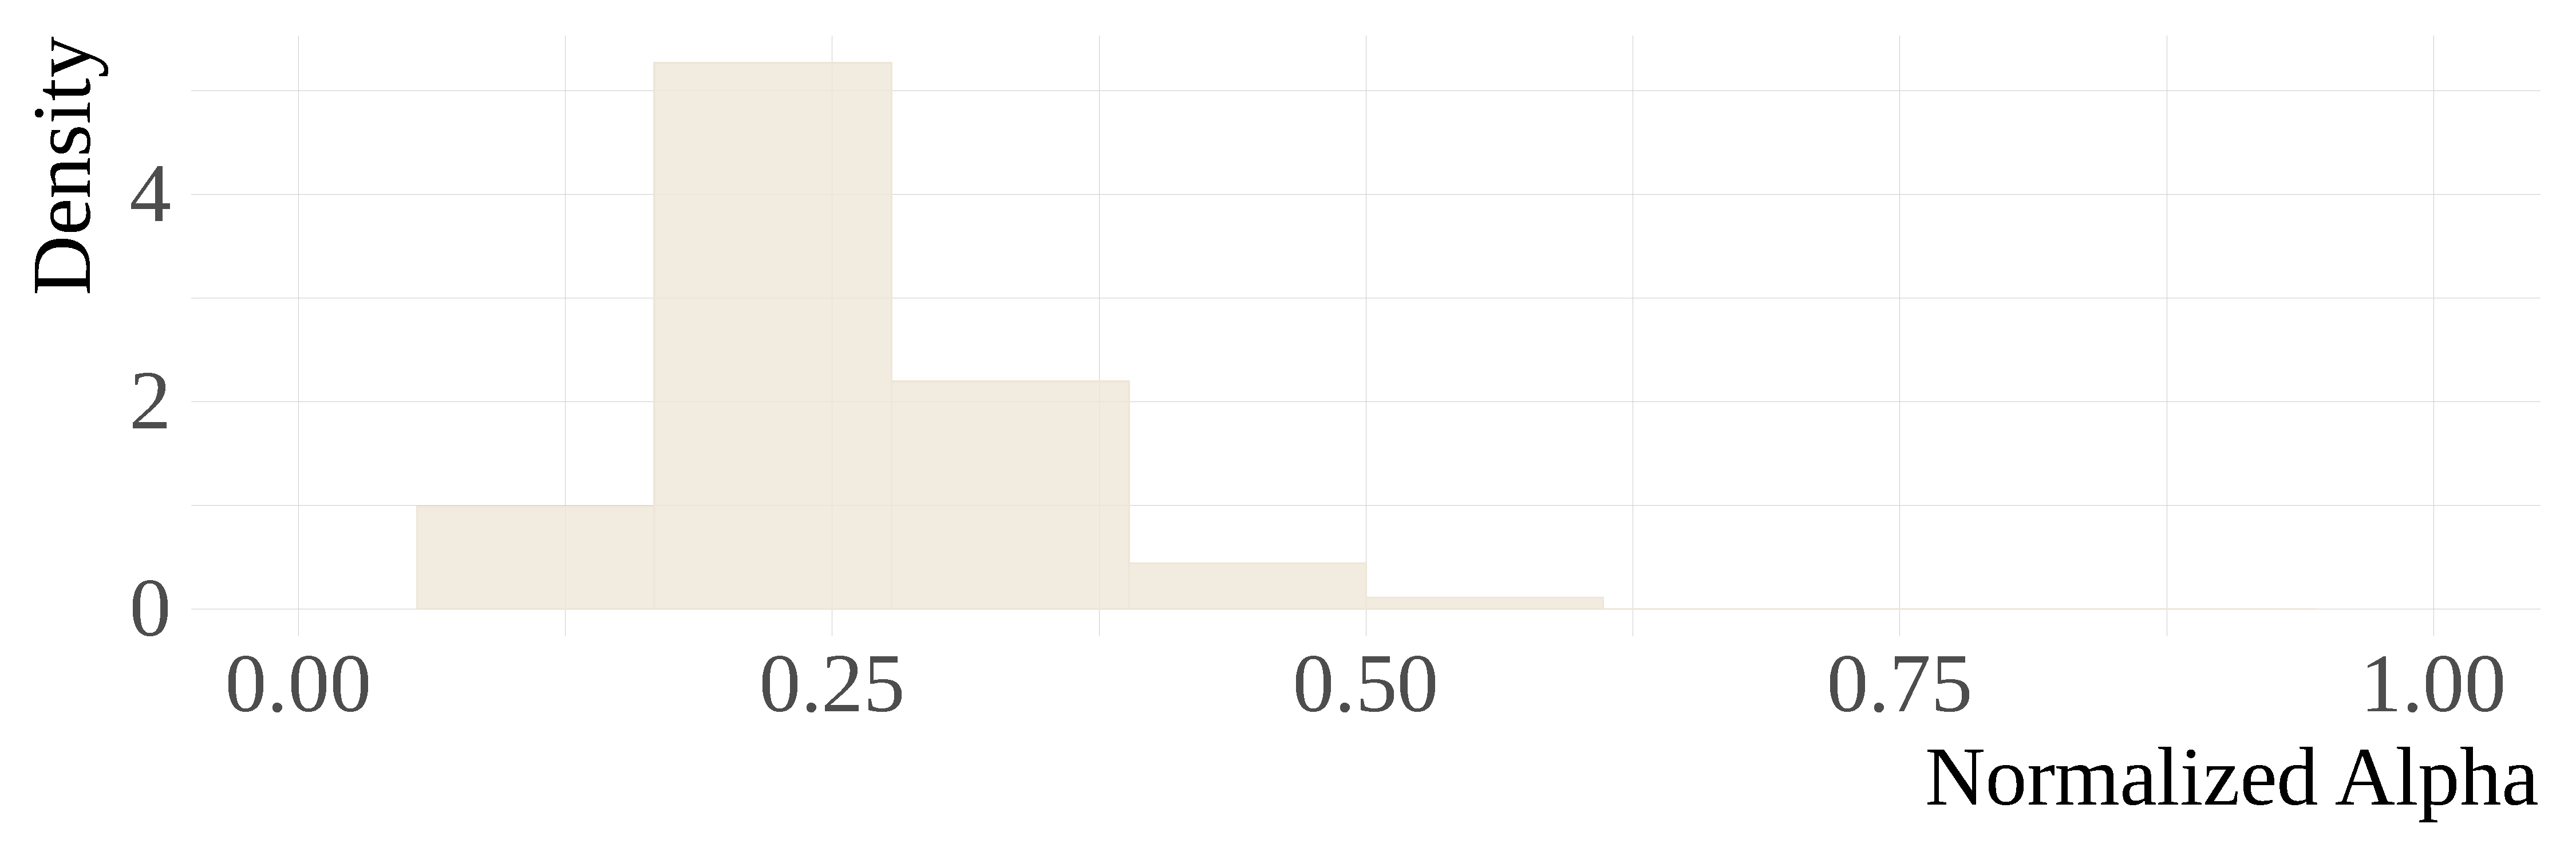
\includegraphics[width = \linewidth]{alpha_ot102_4}}
\subcaptionbox{27 July 2016}{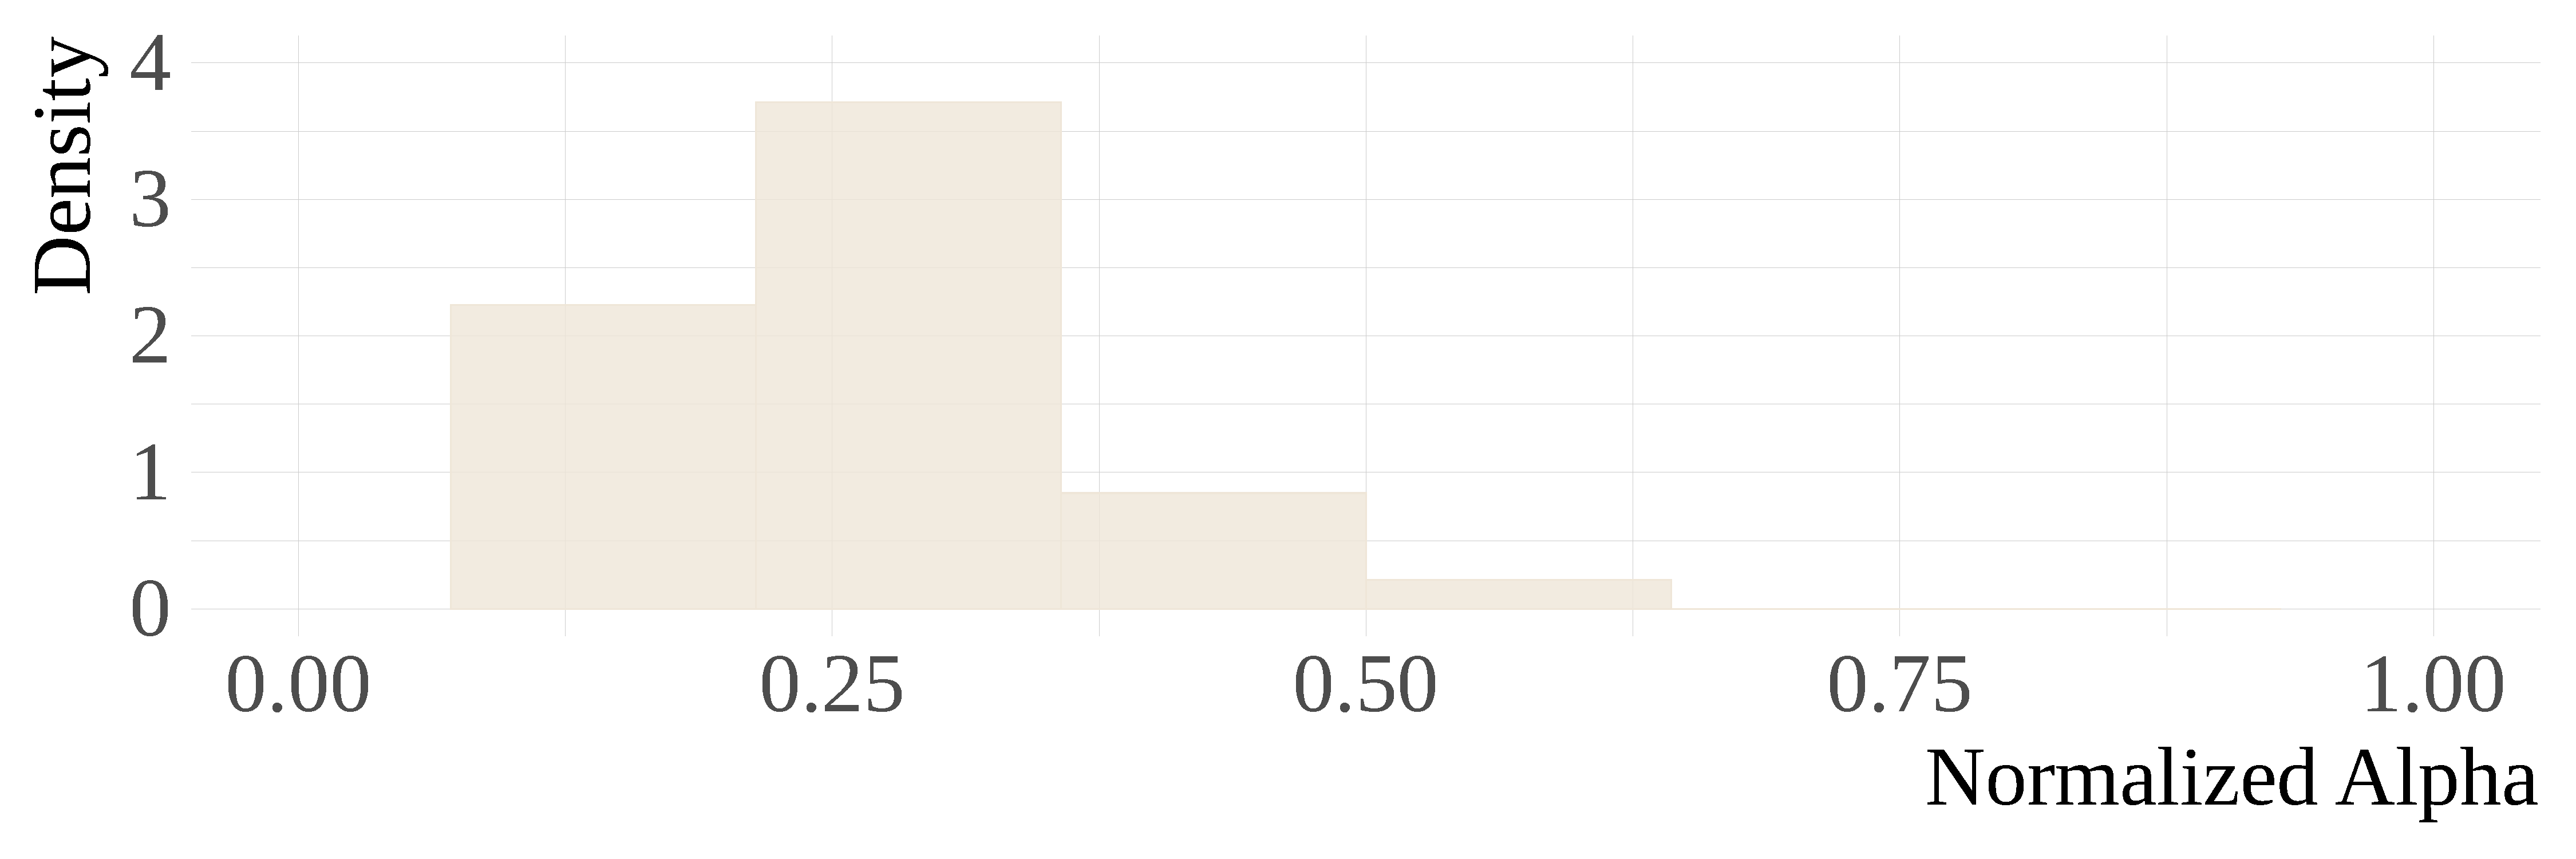
\includegraphics[width = \linewidth]{alpha_ot102_5}}
\caption{Histograms of the geodesic distances between trihedral and the pixels from Oats 102 most similar to trihedral}
\label{fig:histograms_alpha_ot102}
\end{figure}

\begin{figure}[hbt]
\centering
\subcaptionbox{16 May 2016}{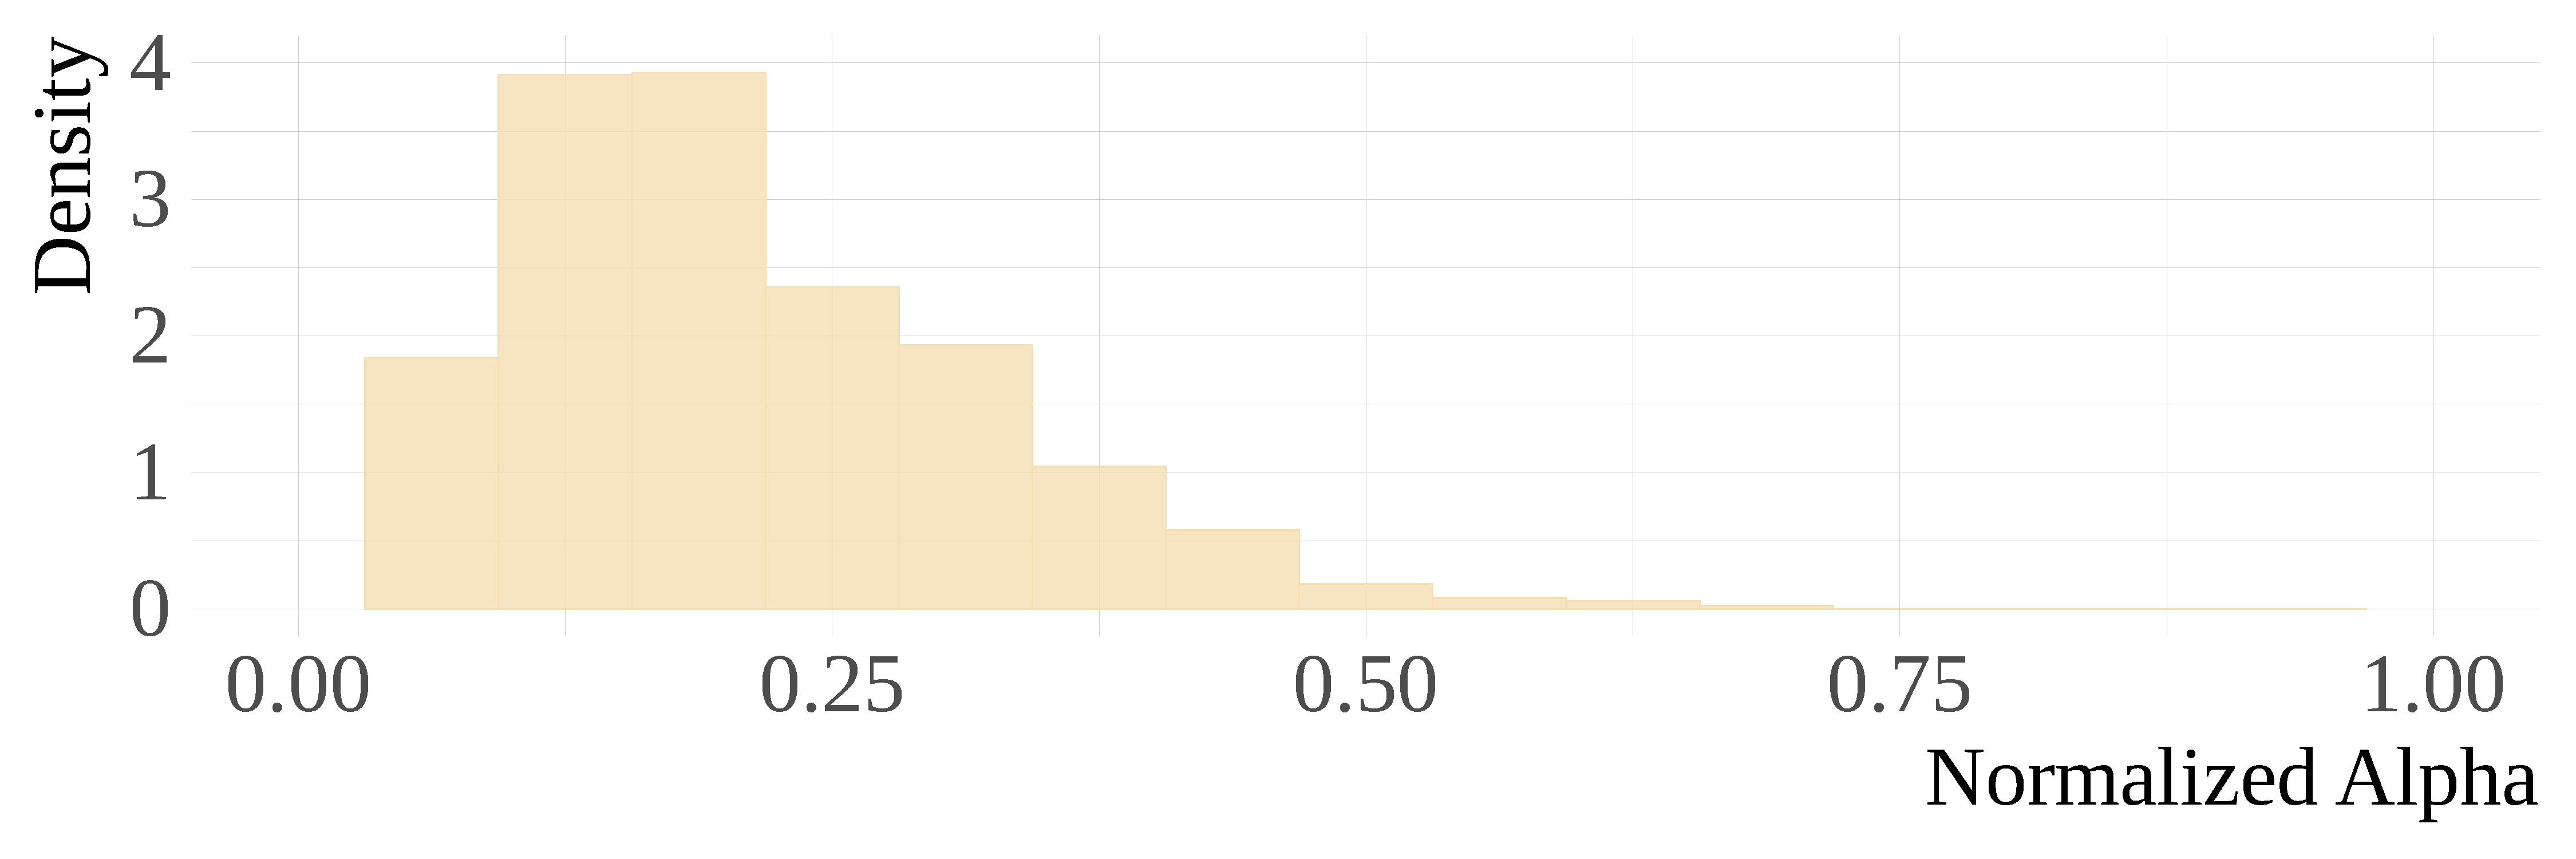
\includegraphics[width = \linewidth]{/alpha_wt104_1}}
\subcaptionbox{09 June 2016}{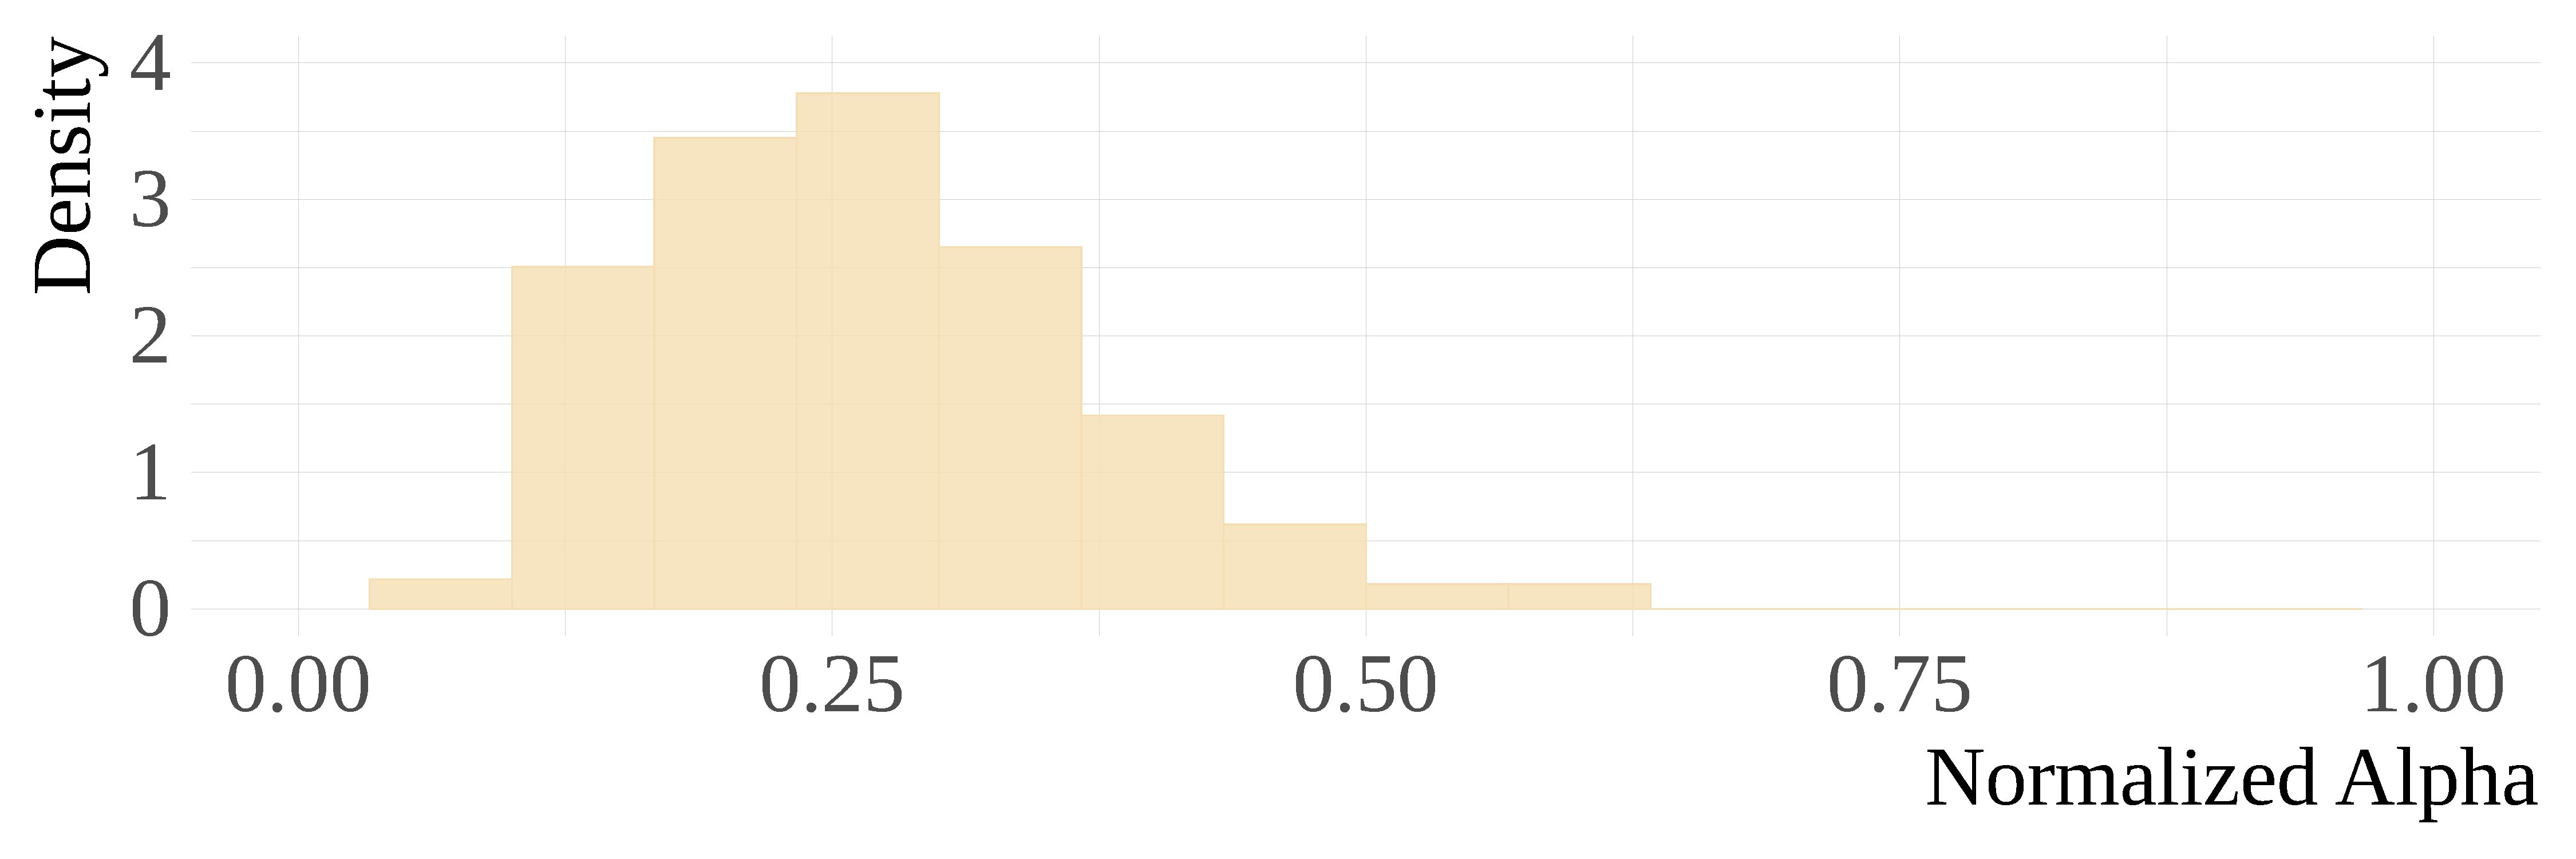
\includegraphics[width = \linewidth]{/alpha_wt104_2}}
\subcaptionbox{03 July 2016}{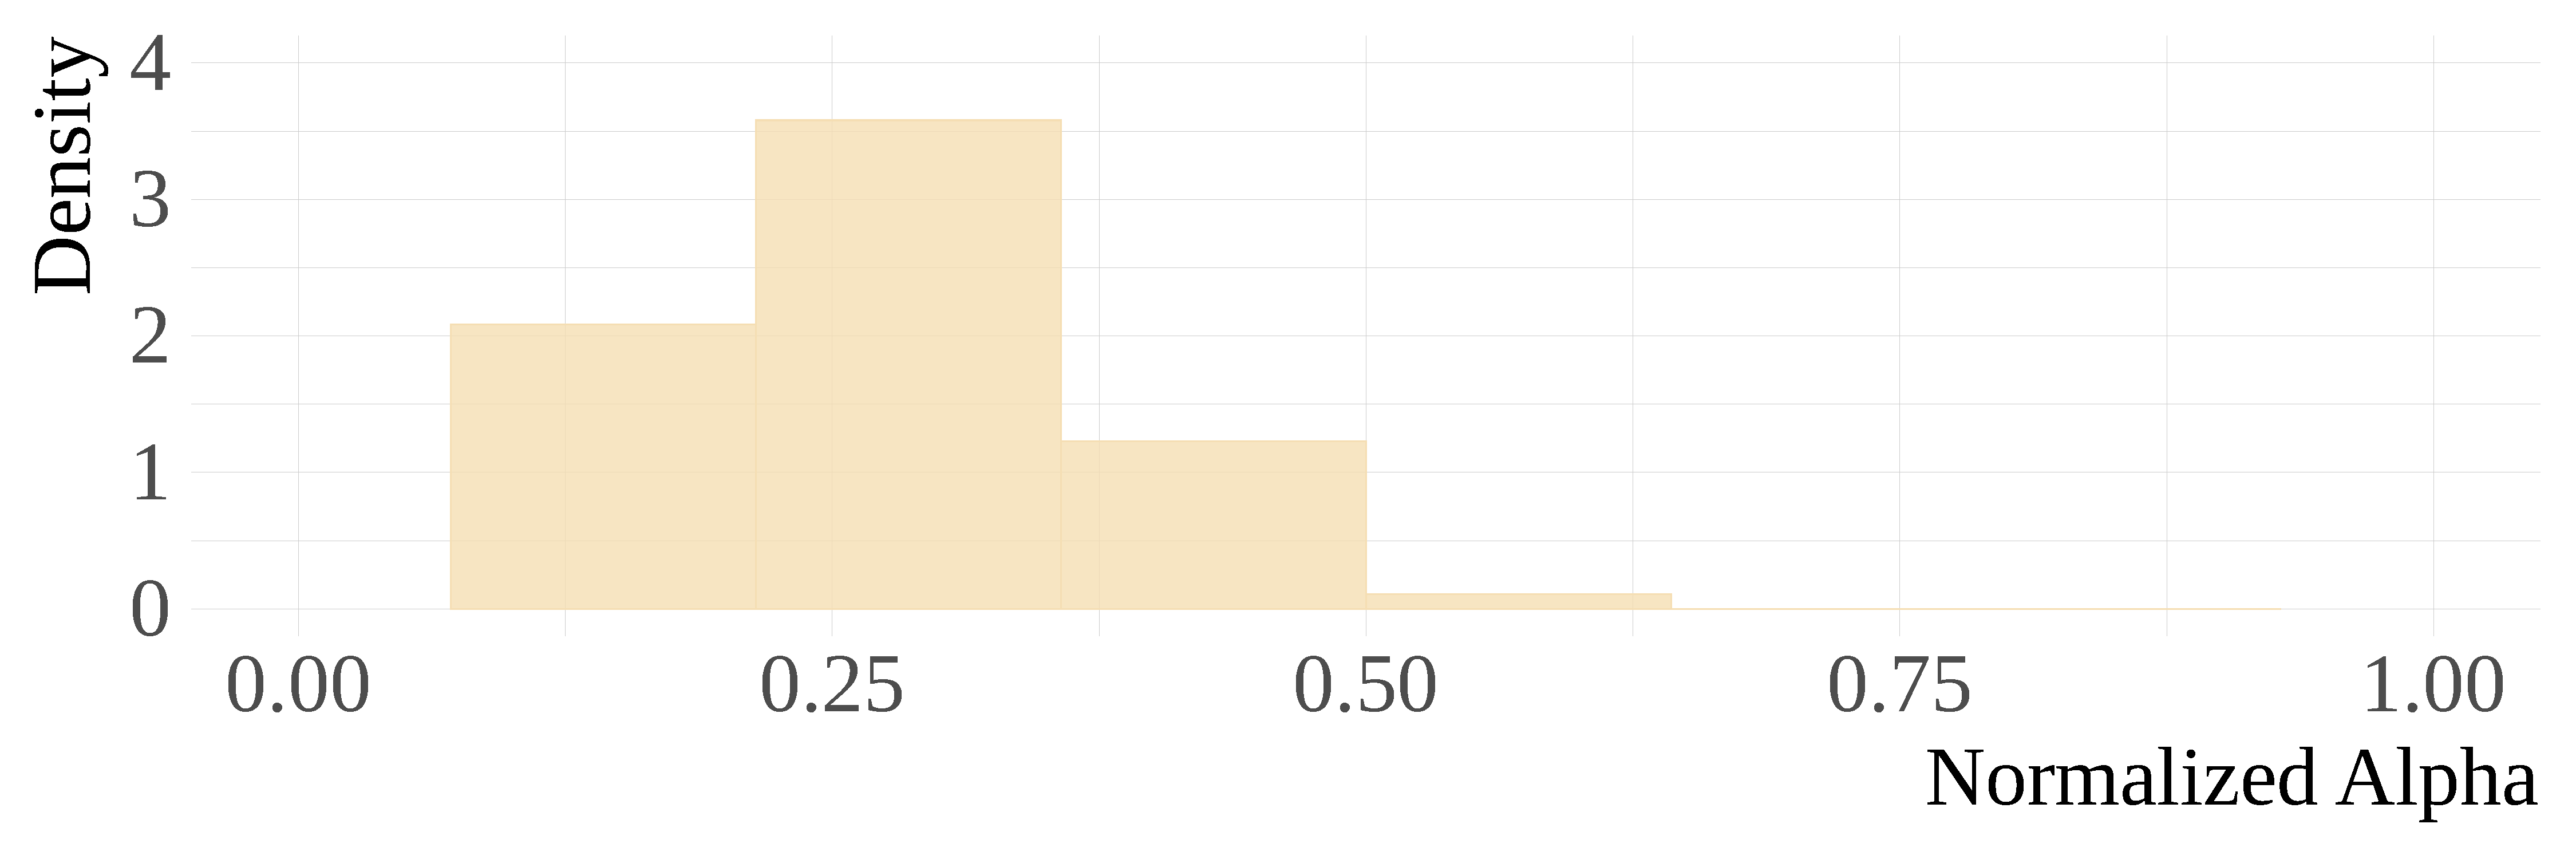
\includegraphics[width = \linewidth]{/alpha_wt104_3}}
\subcaptionbox{27 July 2016}{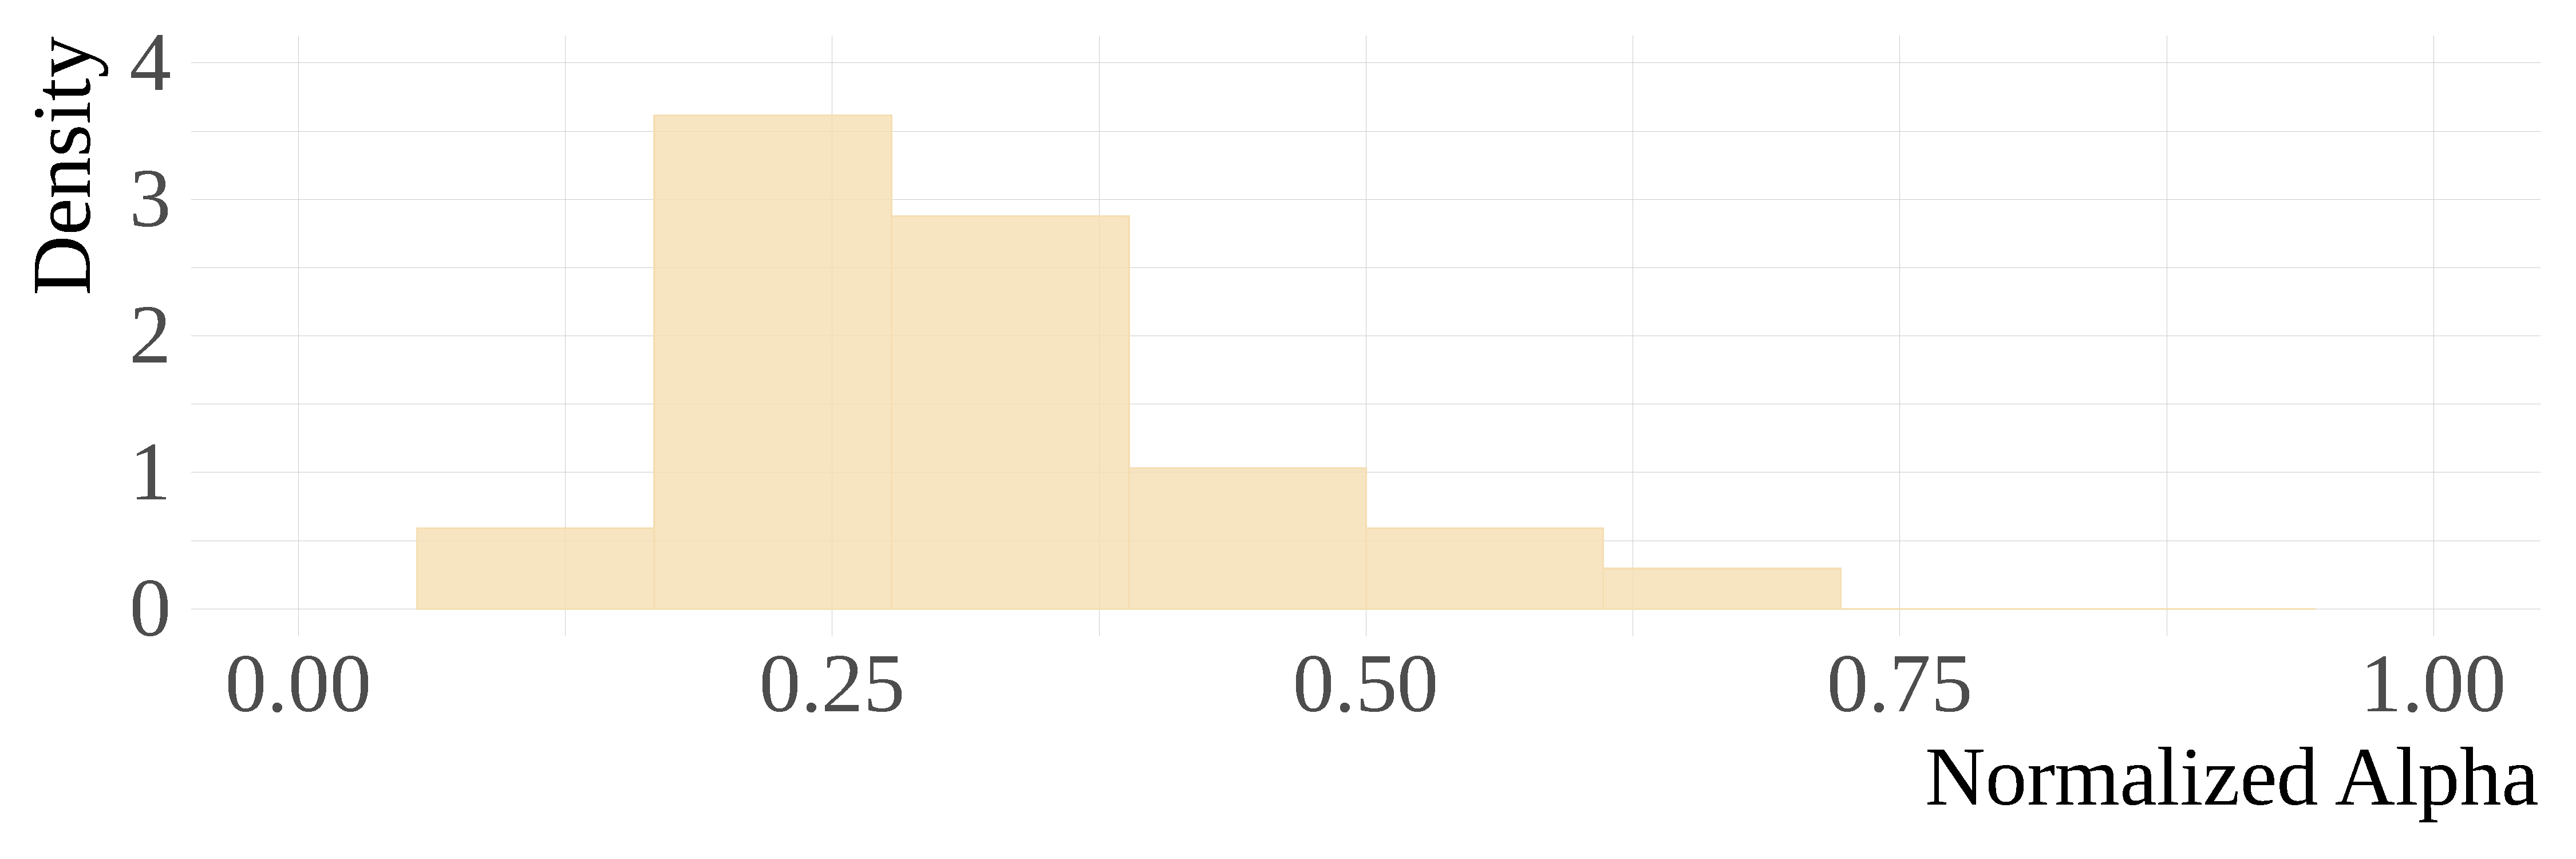
\includegraphics[width = \linewidth]{/alpha_wt104_4}}
\subcaptionbox{20 August 2016}{\includegraphics[width = \linewidth]{/alpha_wt104_5}}
\caption{Histograms of the geodesic distances between trihedral and the pixels from Wheat 104 most similar to trihedral}
\label{fig:histograms_alpha_wt104}
\end{figure}

\begin{table}[hbt]
  \centering
  \caption{$p$-values from Komolgorov-Smirnov Test for normalized alpha from Oats 102}
  \label{tab:pvalues_alpha_ot102}
  \begin{tabular}{lrrrrr}
    \toprule
    \textbf{Day} & \textbf{16 May} & \textbf{09 June} & \textbf{03 July} & \textbf{27 July} & \textbf{20 Aug.}\\ 
                 & \textbf{2016} & \textbf{2016} & \textbf{2016} & \textbf{2016} & \textbf{2016}\\\midrule
    \textbf{Sample size} & 1207 & 991 & 263 & 82 & 66\\
    \textbf{$p$-value} & 0.3504 & 0.2841 & 0.4707 & 0.2933 & 0.3958\\
    \bottomrule
  \end{tabular}
\end{table}

\begin{table}[hbt]
  \centering
  \caption{$p$-values from Komolgorov-Smirnov Test for normalized alpha from Wheat 104}
  \label{tab:pvalues_alpha_wt104}
  \begin{tabular}{lrrrrr}
    \toprule
    \textbf{Day} & \textbf{16 May} & \textbf{09 June} & \textbf{03 July} & \textbf{27 July} & \textbf{20 Aug.}\\ 
                 & \textbf{2016} & \textbf{2016} & \textbf{2016} & \textbf{2016} & \textbf{2016}\\\midrule
    \textbf{Sample size} & 1382 & 413 & 131 & 122 & 116\\
    \textbf{$p$-value} & 0.1795 & 0.8726 & 0.5488 & 0.3261 & 0.7663\\
    \bottomrule
  \end{tabular}
\end{table}

\begin{table}[hbt]
  \centering
  \caption{Maximum Likelihood estimated Beta parameters for normalized alpha from Soybeans 231}
  \label{tab:params_helicity}
  \begin{tabular}{lrrrrr}
    \toprule
    \textbf{Day} & \textbf{16 May} & \textbf{09 June} & \textbf{03 July} & \textbf{27 July} & \textbf{20 Aug.}\\ 
                 & \textbf{2016} & \textbf{2016} & \textbf{2016} & \textbf{2016} & \textbf{2016}\\\midrule
    \textbf{$\hat{\alpha}$} & 3.1092 & 4.1239 & 3.7793 & 4.6720 & 4.8640\\
    \textbf{$\hat{\beta}$} & 11.5536 & 13.6485 & 11.2156 & 13.8374 & 13.8050\\
    \bottomrule
  \end{tabular}
\end{table}

\begin{table}[hbt]
  \centering
  \caption{Maximum Likelihood estimated Beta parameters for normalized alpha from Canola 43}
  \label{tab:params_alpha_cn43}
  \begin{tabular}{lrrrrr}
    \toprule
    \textbf{Day} & \textbf{16 May} & \textbf{09 June} & \textbf{03 July} & \textbf{27 July} & \textbf{20 Aug.}\\ 
                 & \textbf{2016} & \textbf{2016} & \textbf{2016} & \textbf{2016} & \textbf{2016}\\\midrule
    \textbf{$\hat{\alpha}$} & 2.5812 & 4.0304 & 5.6943 & 6.0239 & 6.0750\\
    \textbf{$\hat{\beta}$} & 10.3476 & 13.4359 & 16.1670 & 14.8314 & 15.2520\\
    \bottomrule
  \end{tabular}
\end{table}

\begin{table}[hbt]
  \centering
  \caption{Maximum Likelihood estimated Beta parameters for normalized alpha from Oats 102}
  \label{tab:params_alpha_ot102}
  \begin{tabular}{lrrrrr}
    \toprule
    \textbf{Day} & \textbf{16 May} & \textbf{09 June} & \textbf{03 July} & \textbf{27 July} & \textbf{20 Aug.}\\ 
                 & \textbf{2016} & \textbf{2016} & \textbf{2016} & \textbf{2016} & \textbf{2016}\\\midrule
    \textbf{$\hat{\alpha}$} & 3.1005  & 2.9157 & 4.9835 & 7.2026 & 6.8227\\
    \textbf{$\hat{\beta}$} & 10.5901 & 10.3148 & 14.9391 & 21.4717 & 18.5422\\
    \bottomrule
  \end{tabular}
\end{table}

\begin{table}[hbt]
  \centering
  \caption{Maximum Likelihood estimated Beta parameters for normalized alpha from Wheat 104}
  \label{tab:params_alpha_wt104}
  \begin{tabular}{lrrrrr}
    \toprule
    \textbf{Day} & \textbf{16 May} & \textbf{09 June} & \textbf{03 July} & \textbf{27 July} & \textbf{20 Aug.}\\ 
                 & \textbf{2016} & \textbf{2016} & \textbf{2016} & \textbf{2016} & \textbf{2016}\\\midrule
    \textbf{$\hat{\alpha}$} & 2.7237 & 4.6521 & 7.8296 & 4.1457 & 5.7762\\
    \textbf{$\hat{\beta}$} & 10.2709 & 12.8761 & 20.2683 & 9.2153 & 14.3660\\
    \bottomrule
  \end{tabular}
\end{table}

Additionally, we performed a separability test based on the Hellinger distance between the original samples assuming the Beta distribution.
Table~\ref{tab:pvalues_sep_alpha_sb231} shows the $p$-values of the null hypothesis that each pair comes from the same law.
We observe that at level $0.05$, the only null hypothesis that cannot be rejected is that the data from the two last dates come from the same law.

\begin{table}[hbt]
  \footnotesize
  \centering
  \caption{$p$-values from Separability Test for normalized alpha from Soybeans 231}
  \label{tab:pvalues_sep_alpha_sb231}
  \begin{tabular}{ccccc}
  \toprule
& \textbf{09 June} & \textbf{03 July} & \textbf{27 July} & \textbf{20 Aug.}\\ \midrule
  \textbf{16 May}  & $7.47 \times 10^{-8}$ & $9.22 \times 10^{-12}$ & $5.16 \times 10^{-21}$ & $1.31 \times 10^{-24}$ \\
  \textbf{09 June}  & --- & $2.64 \times 10^{-3}$ & $4.55 \times 10^{-4}$ & $1.76 \times 10^{-6}$ \\
  \textbf{03 July}  & --- & --- & $4.32 \times 10^{-2}$ & $1.07 \times 10^{-2}$\\
  \textbf{27 July}  & --- & --- & --- & $3.64 \times 10^{-1}$ \\
  \bottomrule
  \end{tabular}
\end{table}

\begin{table}[hbt]
  \footnotesize
  \centering
  \caption{$p$-values from Separability Test for normalized alpha from Canola 43}
  \label{tab:pvalues_sep_alpha_cn43}
  \begin{tabular}{ccccc}
  \toprule
  & \textbf{09 June} & \textbf{03 July} & \textbf{27 July} & \textbf{20 Aug.}\\ \midrule
  \textbf{16 May}  & $1.86 \times 10^{-19}$ & $4.07 \times 10^{-36}$ & $2.75 \times 10^{-25}$ & $9.79 \times 10^{-27}$ \\
  \textbf{09 June}  & --- & $5.28 \times 10^{-8}$ & $2.94 \times 10^{-10}$ & $3.06 \times 10^{-10}$ \\
  \textbf{03 July}  & --- & --- & $1.48 \times 10^{-2}$ & $3.21 \times 10^{-2}$\\
  \textbf{27 July}  & --- & --- & --- & $9.39 \times 10^{-1}$ \\
  \bottomrule
  \end{tabular}
\end{table}

\begin{table}[hbt]
  \footnotesize
  \centering
  \caption{$p$-values from Separability Test for normalized alpha from Oats 102}
  \label{tab:pvalues_sep_alpha_ot102}
  \begin{tabular}{ccccc}
  \toprule
  & \textbf{09 June} & \textbf{03 July} & \textbf{27 July} & \textbf{20 Aug.}\\ \midrule
  \textbf{16 May}  & $2.77 \times 10^{-1}$ & $3.71 \times 10^{-8}$ & $2.18 \times 10^{-7}$ & $7.32 \times 10^{-7}$ \\
  \textbf{09 June}  & --- & $2.08 \times 10^{-10}$ & $1.47 \times 10^{-8}$ & $5.45 \times 10^{-8}$ \\
  \textbf{03 July}  & --- & --- & $1.09 \times 10^{-1}$ & $1.01 \times 10^{-1}$\\
  \textbf{27 July}  & --- & --- & --- & $4.08 \times 10^{-1}$ \\
  \bottomrule
  \end{tabular}
\end{table}

\begin{table}[hbt]
  \footnotesize
  \centering
  \caption{$p$-values from Separability Test for normalized alpha from Wheat 104}
  \label{tab:pvalues_sep_alpha_wt104}
  \begin{tabular}{ccccc}
  \toprule
  & \textbf{09 June} & \textbf{03 July} & \textbf{27 July} & \textbf{20 Aug.}\\ \midrule
  \textbf{16 May}  & $4.24 \times 10^{-27}$ & $2.61 \times 10^{-24}$ & $3.08 \times 10^{-19}$ & $1.32 \times 10^{-17}$ \\
  \textbf{09 June}  & --- & $5.42 \times 10^{-4}$ & $2.70 \times 10^{-4}$ & $5.58 \times 10^{-2}$ \\
  \textbf{03 July}  & --- & --- & $3.31 \times 10^{-5}$ & $1.58 \times 10^{-1}$\\
  \textbf{27 July}  & --- & --- & --- & $3.24 \times 10^{-2}$ \\
  \bottomrule
  \end{tabular}
\end{table}

\subsection{Geodesic Helicity}

%In the figures \ref{fig:histograms_helicity} the histograms of normalized helicities computed for each sample are shown. For these, goodness-of-fit tests were performed -- through Komolgorov-Smirnov Test -- with Beta distribution, whose $p$-values are shown in table \ref{tab:pvalues_helicities}.

% \begin{figure}[hbt]
%     \centering
%     \subcaptionbox{16 May 2016}{\includegraphics[width = \linewidth]{Figures/Soybeans_231/helicity_sb231_1}}
%     \subcaptionbox{09 June 2016}{\includegraphics[width = \linewidth]{Figures/Soybeans_231/helicity_sb231_2}}
%     \subcaptionbox{03 July 2016}{\includegraphics[width = \linewidth]{Figures/Soybeans_231/helicity_sb231_3}}
%     \subcaptionbox{27 July 2016}{\includegraphics[width = \linewidth]{Figures/Soybeans_231/helicity_sb231_4}}
%     \subcaptionbox{20 August 2016}{\includegraphics[width = \linewidth]{Figures/Soybeans_231/helicity_sb231_5}}
%     \caption{Histograms of the normalized geodesic helicities}
%     \label{fig:histograms_helicity}
% \end{figure}

% \begin{table}[hbt]
%   \centering
%   \caption{Maximum Likelihood estimated Beta parameters for normalized helicity from Soybeans 231}
%   \label{tab:params_helicity}
%   \begin{tabular}{lrrrrr}
%     \toprule
%     \textbf{Day} & \textbf{16 May} & \textbf{09 June} & \textbf{03 July} & \textbf{27 July} & \textbf{20 Aug.}\\ 
%                  & \textbf{2016} & \textbf{2016} & \textbf{2016} & \textbf{2016} & \textbf{2016}\\\midrule
%     \textbf{$\hat{\alpha}$} & 2.0984 & 2.4793 & 3.0300 & 2.8211 & 3.2862\\
%     \textbf{$\hat{\beta}$} & 26.0484 & 18.0347 & 17.0150 & 16.9940 & 17.6112\\
%     \bottomrule
%   \end{tabular}
% \end{table}


% \begin{table}[hbt]
%   \centering
%   \caption{$p$-values from Komolgorov-Smirnov Test for normalized helicity from Soybeans 231}
%   \label{tab:pvalues_helicities}
%   \begin{tabular}{lrrrrr}
%     \toprule
%     \textbf{Day} & \textbf{16 May} & \textbf{09 June} & \textbf{03 July} & \textbf{27 July} & \textbf{20 Aug.}\\
%                  & \textbf{2016} & \textbf{2016} & \textbf{2016} & \textbf{2016} & \textbf{2016}\\\midrule
%     \textbf{$p$-value} & 0.0018  & 0.0118 & 0.9812 & 0.2525 & 0.3358\\
%     \bottomrule
%   \end{tabular}
% \end{table}

\section{Conclusion}
%The conclusion goes here. This is the beginning paper to look at~\cite{Ratha2020}.

% if have a single appendix:
%\appendix[Proof of the Zonklar Equations]
% or
%\appendix  % for no appendix heading
% do not use \section anymore after \appendix, only \section*
% is possibly needed

% use appendices with more than one appendix
% then use \section to start each appendix
% you must declare a \section before using any
% \subsection or using \label (\appendices by itself
% starts a section numbered zero.)
%


\section*{Acknowledgment}


The authors would like to thank...

\nocite{ClassificationPolSARGeodesic,AGeneralizedVolumeScatteringModelBasedVegetationIndexfromPolarimetricSARData2019,NovelTechniquesforBuiltupAreaExtractionfromPolarimetricSARImages2019,APolSARScatteringPowerFactorizationFrameworkandNovelRollInvariantParametersBasedUnsupervisedClassificationSchemeUsingaGeodesicDistanceinpress,TheKennaughElementFrameworkforMultiScaleMultiPolarizedMultiTemporalandMultiFrequencySARImagePreparation,ScatteringCharacteristicsXCL-BandPolSARData,RadarTargetRecognitionBasedonModifiedCharacteristicPolarizationStates,RedevelopmentofKennaughsTargetCharacteristicPolarizationStateTheoryUsingthePolarizationTransformationRationFormalismfortheCoherentCase}

\bibliographystyle{IEEEtran}
\bibliography{../../../../Bibliography/references}


% % that's all folks
\end{document}